%                                     MMMMMMMMM                                         
%                                                                             
%  MMO    MM   MMMMMM  MMMMMMM   MM    MMMMMMMM   MMD   MM  MMMMMMM MMMMMMM   
%  MMM   MMM   MM        MM     ?MMM              MMM$  MM  MM         MM     
%  MMMM 7MMM   MM        MM     MM8M    MMMMMMM   MMMMD MM  MM         MM     
%  MM MMMMMM   MMMMMM    MM    MM  MM             MM MMDMM  MMMMMM     MM     
%  MM  MM MM   MM        MM    MMMMMM             MM  MMMM  MM         MM     
%  MM     MM   MMMMMM    MM   MM    MM            MM   MMM  MMMMMMM    MM
%
%
%            - META-NET Language Whitepaper | Hungarian paper -
%
% ----------------------------------------------------------------------------

\documentclass[]{../../metanetpaper}

\usepackage{booktabs}
\usepackage{longtable}
\usepackage{tabulary}
\usepackage{tabularx}
\usepackage{rotating}
\usepackage{makecell}
\usepackage{multirow}
\usepackage{colortbl}
\usepackage{polyglossia}
\usepackage{multicol,framed,lipsum}
\setotherlanguages{hungarian,english}

%!TEX TS-program = xelatex
\RequireXeTeX %Force XeTeX check

\title{A magyar nyelv a digitális korban --- The Hungarian Language in the Digital Age}

\subtitle{White Paper Series --- Fehér könyvek sorozat}

\author{
  Simon Eszter~ {\small MTA Nyelvtudományi Intézet}\\
  Lendvai Piroska~ {\small MTA Nyelvtudományi Intézet}\\
  Németh Géza~ {\small BME} \\
  Olaszy Gábor~ {\small BME}\\
  Vicsi Klára~ {\small BME}\\
}
\editors{
  Simon Eszter, Lendvai Piroska\\(szerkesztők, \textcolor{grey1}{editors})
}

\begin{document}

\renewcommand*{\figureformat}{\sffamily\thefigure\autodot}

\maketitle

\null
\pagestyle{empty} 

\FundingLNotice{\selectlanguage{hungarian}\vskip2mm
  Lorem ipsum dolor sit amet, consectetur adipisicing elit, sed do eiusmod tempor incididunt ut labore et dolore magna aliqua. Ut enim ad minim veniam, quis nostrud exercitation ullamco laboris nisi ut aliquip ex ea commodo.
  
  \bigskip

  A fehér könyv megírását az Európai Bizottság 7. keretprogramja és ICT PSP programja támogatta a T4ME (szerződésszám: 249119), a CESAR (szerződésszám: 271022), a METANET4U (szerződésszám: 270893) és a META-NORD (szerződésszám: 270899) projekteken keresztül.}

\FundingRNotice{\selectlanguage{english}
  The authors of this document are grateful to the authors of the White Paper on German for permission to re-use selected language-independent materials from their document. \cite{lwpgerman} 
  
  \bigskip

  The development of this white paper has been funded by the Seventh Framework Programme and the ICT Policy Support Programme of the European Commission under the contracts T4ME (Grant Agreement 249119), CESAR (Grant Agreement 271022), META\-NET4U (Grant Agreement 270893) and META-NORD (Grant Agreement 270899).}

\makefundingnotice

\pagenumbering{Roman} 
\setcounter{page}{5}
\pagestyle{scrheadings}

\cleardoublepage

% --------------------------------------------------------------------------

\bsection*{Előszó --- Preface}

\begin{Parallel}[c]{78mm}{78mm}
\ParallelLText{
\selectlanguage{hungarian}\vskip2mm
Ez a fehér könyv egy sorozat részét képezi, amelynek célja, hogy felhívja a figyelmet a nyelvtechnológiára és az abban rej\-lő lehetőségekre. Elsősorban oktatókat, újságírókat, politikusokat és nyelvi kö\-zös\-sé\-ge\-ket szólít meg. Az európai nyelvek nyelvtechnológiai feldolgozottsága és a nyelvtechnológia elterjedtsége meglehetősen eltérő. Ezért a nyelvtechnológia fej\-lődéséhez és a kutatás elősegítéséhez szükséges lépések is nyelvenként mások és mások, és olyan különféle tényezőkön múlnak, mint az adott nyelv összetettsége, vagy a nyelvet hasz\-ná\-ló közösség nagysága.

A META-NET, az Európai Bizottság által alapított hálózat felmérést végzett a rendelkezésre álló nyelvi erőforrásokról és technológiákról (lásd a \pageref{whitepaperseries}.~oldalt). Ez a felmérés a 23 hivatalos európai nyelv mellett egyéb nemzeti és regionális nyelvekre is kiterjed, és eredményei rámutatnak az egyes nyelvek terén fellelhető kutatási hiányosságokra. Egy, a jelenlegi helyzetet bemutató részletes szakértői elemzés és értékelés segíthet a további kutatások hatásának maximalizálásában.

A META-NET 33 ország 54 kutatóközpontjából áll (2011.~novemberi helyzet szerint, lásd a \pageref{metanetmembers}.~oldalt), akik a területtel foglalkozó vállalkozásokkal, kormányzati szervekkel, kutatószervezetekkel, szoftvercégekkel, szolgáltatókkal és európai egyetemekkel dolgoznak együtt. Egységes technológiai víziót alkotva egy olyan stratégiai kutatási terv létrehozásán dolgoznak, amelyben megfogalmazzák, hogyan tudnak a nyelvtechnológiai alkalmazások a kutatási hiányosságokon enyhíteni a 2020-ig terjedő időszakban.}

\ParallelRText{\selectlanguage{english}\vskip-2mm
This white paper is part of a series that promotes knowledge about language technology and its potential. It addresses journalists, politicians, language communities, educators and others. The availability and use of language technology in Europe varies between languages. Consequently, the actions that are required to further support research and development of language technologies also differ. The required actions depend on many factors, such as the complexity of a given language and the size of its community.

META-NET, a Network of Excellence funded by the European Commission, has conducted an analysis of current language resources and technologies in this white paper series (p.~\pageref{whitepaperseries}). The analysis focused on the 23 official European languages as well as other important national and regional languages in Europe. The results of this analysis suggest that there are tremendous deficits in technology support and significant research gaps for each language. The given detailed expert analysis and assessment of the current situation will help maximise the impact of additional research.

As of November 2011, META-NET consists of 54 research centres from 33 European countries (p.~\pageref{metanetmembers}). META-NET is working with stakeholders from economy (software companies, technology providers, users), government agencies, research organisations, non-governmental organisations, language communities and European universities. Together with these communities, META-NET is creating a common technology vision and strategic research agenda for multilingual Europe 2020.} 
\ParallelPar
\end{Parallel}

% --------------------------------------------------------------------------

\cleardoublepage

\bsection*{Tartalomjegyzék --- Table of Contents}

\tableofcontents

\addtocontents{toc}{\protect\thispagestyle{empty}\protect}
\addtocontents{toc}{{\Large\textsf{\centerline{A MAGYAR NYELV A DIGITÁLIS KORBAN}}\par}}

% --------------------------------------------------------------------------

\cleardoublepage

\setcounter{page}{1}
\pagenumbering{arabic} 
\pagestyle{scrheadings}

\ssection[Vezetői összefoglaló]{Vezetői összefoglaló}

\selectlanguage{hungarian}

\begin{multicols}{2}
Az elmúlt 60 évben Európa jelentős politikai és gazdasági szervezetté vált, ám kulturálisan és nyelvészetileg még mindig nagyon változatos. Ez azt jelenti, hogy a mindennapi kommunikáció Európa polgárai, például a portugálok és a lengyelek vagy az olaszok és az izlandiak között, mind az üzleti, mind a politikai szférában elkerülhetetlenül nyelvi akadályokba ütközik. Az EU intézményei körülbelül évi egy milliárd eurót költenek a többnyelvűség fenntartására, vagyis tolmácsolásra és fordításra. Tényleg ilyen terhet kell ennek jelentenie? A modern nyelvtechnológia és a nyelvészeti kutatások jelentősen hozzá tudnak járulni ezen akadályok legyőzéséhez. Az intelligens eszközök és alkalmazások kombinációjával a nyelvtechnológia a jövőben képes lesz segíteni az európai polgárokat abban, hogy könnyen beszélhessenek és üzletelhessenek egymással -- még akkor is, ha nem beszélnek közös nyelvet.

\boxtext{A nyelvtechnológia hidakat épít.}

A magyar gazdaságnak sok előnye származik az európai közös piacból, de a nyelvi határok az üzletnek is határt szabhatnak, különösen a kis- és középvállalkozások esetében, akik nem rendelkeznek megfelelő pénzügyi háttérrel a helyzet megváltoztatásához. A többnyelvű Európa egyedüli (és elképzelhetetlen) alternatívája egy egységes nyelv használata lenne, amely átvenné a vezető szerepet, és lecserélné az összes többit. 

A nyelvi akadályok legyőzésének klasszikus útja a nyelvtanulás. Viszont technikai támogatás nélkül 23 hivatalos és 60 egyéb európai nyelv elsajátítása leküzdhetetlen akadályt gördít az európai polgárok gazdasági, politikai élete és tudományos fej\-lődése elé. 

A megoldást a kulcsfontosságú tech\-no\-ló\-gi\-ák építése adja. Ezen tech\-no\-ló\-gi\-ák hatalmas előnyére válnak az európai szereplőknek, nem csak a közös európai piacon belül, hanem az azon kívüli, különösen a fejlődő országokkal való kereskedelmi kapcsolatokban is. Ahhoz, hogy elérjük ezt a célt, és megvédjük Európa kulturális és nyelvi sokszínűségét, szisztematikus elemzést kell végeznünk Európa nyelveinek különlegességeiről és a jelenlegi nyelvtechnológiai támogatottságukról. Így végül a nyelvtechnológiai megoldások hidakat fognak alkotni Európa nyelvei között.  

A jelenleg piacon lévő gépi fordító- és beszédfeldolgozó szoftverek még sajnos elégtelennek bizonyulnak a címben megfogalmazott cél eléréséhez. A piac do\-mi\-náns alakítói jelenleg főként az Észak-Amerikában működő profitorientált ma\-gán\-cé\-gek közül kerülnek ki. Az EU már a hetvenes évek végén felismerte, hogy a nyelvtechnológia az európai egység mozgatórugója, és elindította első pro\-jekt\-jeit, többek között az EUROTRA-t. Ugyanakkor egyre gyakoribbá váltak az értékes eredményeket hozó, nemzeti szin\-ten létrehozott projektek is, amelyek azonban sosem koncentrálódtak egységes, európai tudássá. Ezzel a részleges teljesítményeket eredményező hozzáállással szemben a közelmúltban (a 22 hivatalos nyelvvel rendelkező) Indiában és (a 11 hivatalos nyelvvel rendelkező) Dél-Afrikában már hosszú távú nemzeti nyelv\-tech\-no\-ló\-giai és nyelvészeti programok létrehozására törekednek. 

\boxtext{A nyelvtechnológia a jövő kulcsa.}

A nyelvtechnológia mai központi szereplői a kevésbé pontos statisztikai módszerekben bíznak, amelyek nem használnak mélyebb nyelvészeti módszereket és tudást. Például mondatok gépi fordításakor az emberek által már lefordított mondatok közül válogatnak. Ennek megfelelően a kimenet minősége leginkább az elérhető korpuszok nagyságától és minőségétől függ. Míg az egyszerű mondatok automatikus fordítása a kellően nagy méretű korpuszokkal rendelkező nyelvek esetében eredményes módszer lehet, a bonyolultabb szerkezetű mondatok, illetve a kevés re\-fe\-ren\-cia\-korpusszal rendelkező nyelvek ese\-té\-ben a módszer kudarcra van ítélve. 

Az Európai Unió ezért olyan projektek létrehozását tűzte ki célul, mint az EuroMatrix és az EuroMatrixPlus (2006 óta), valamint az iTranslate4 (2010 óta), amelyek alapvető alkalmazott kutatásokra és a minőségi nyelvtechnológiai kutatások alapjául szolgáló erőforrások létrehozására koncentrálnak. Az európai nyelveket átfogó alkalmazások létrehozásának egyedüli módja a nyelvek mélyebb szerkezeti tulajdonságainak vizsgálata.  

Egyes európai kutatások ezen a területen már számos sikert értek el. Például az Európai Unió által használt nyílt forráskódú MOSES gépi fordítót főként az európai kutatásokra építve fejlesztették ki. Az európai kutatási stratégia egyik célja a saját eredményekre való építés mellett a piacra csekély hatást kifejtő elszigetelt kutatási tevékenységek összefogása. Napjaink egyik alapvető stratégiája az erő\-fe\-szí\-té\-sek egyesítése: a 2010 márciusában kezdődött iTranslate4.eu projekt célja olyan gépi fordító szolgáltatás nyújtása, amely nemcsak lefedi az Európai Unió összes nyelvét, hanem az összes nyelvpár esetében a mindenkori legjobb minőségű fordítást is adja. Ezt a tervet az Európa legjobb gépifordító-rendszereinek működtetői által létrehozott konzorcium valósítja meg, amelynek tagjai legalább egy nyelvpár legjobb fordítását biztosítják. A legkorábbi erőfeszítések gazdasági eredményét az üzleti integrációk viszonylag magas száma is tükrözi. Például az 1984-ben létrehozott Tradost 2005-ben az egyesült királysági érdekeltségű SDL vette meg.

\boxtext{A nyelvtechnológia az európai egység megteremtésének elősegítője.}

Az eddigiek alapján elmondható, hogy a mai hibrid nyelvtechnológia, amely ötvözi a mély elemzést és a statisztikai módszereket, képes lehet az európai nyel\-vek közötti kapcsolat létrehozására. Ahogy a fehér könyvek sorozata is bizonyítja, az EU egyes tagállamai között jelentős különbség mutatkozik a nyelvészeti kutatások és nyelvi megoldások fej\-lett\-sé\-gé\-ben. Bár számos technológia és erőforrás áll rendelkezésre a magyar nyelvre, ahhoz, hogy valóban hatékony nyelvtechnológiai megoldásokat használhassunk a mindennapi életben, további kutatásokra van szükség.

A META-NET hosszú távú célja jó mi\-nő\-sé\-gű nyelvtechnológia bevezetése minden nyelvre, a politikai és gazdasági egység elérésének érdekében. A technológia segíthet a meglévő határok ledöntésében és hidak építésében Európa nyelvei között. Ennek érdekében a jövőben minden döntéshozónak, a politika, a kutatás, a gazdaság és a társadalom terén egyaránt egyesítenie kell erőit. 

Jelen fehér könyvek sorozat kiegészíti a META-NET egyéb stratégiai te\-vé\-keny\-sé\-ge\-it (további információért lásd az \ref{meta-net_hu}.~fejezetet). Friss információk a META-NET víziójáról \cite{Meta1}, tevékenységéről, továbbá a Stratégiai Kutatási Terv aktuális ver\-zi\-ó\-ja elérhető a META-NET weboldalán: http://www.meta-net.eu.
\end{multicols}

\clearpage

% --------------------------------------------------------------------------

\ssection[Veszélyben a nyelveink: Kihívás a nyelvtechnológiának]{Veszélyben a nyelveink:\newline Kihívás a nyelvtechnológiának}

\begin{multicols}{2}

Digitális forradalom szemtanúi vagyunk, amely drámaian befolyásolja a kommunikációt és a társadalmat. A digitális és hálózati kommunikációs technológia legújabb vívmányait sokszor Gutenberg invenciójához, a nyomtatás feltalálásához hasonlítják. Mit sugall nekünk ez az analógia az európai információs társadalom és főleg nyelveink jövőjéről? 

\boxtext{Digitális forradalom szemtanúi vagyunk, amelyet Gutenberg invenciójához, a nyomtatás feltalálásához hasonlítanak.}

Gutenberg találmánya után a kommunikációban és tudáscserében a következő nagy áttörést Luther Biblia-fordítása jelentette. Az ezt követő századokban a különböző technikák fejlődése segítette a hatékonyabb nyelvi feldolgozást és tu\-dás\-cse\-rét:

\medskip
\begin{itemize}
\item A nagy nyelvek helyesírási és nyelvtani szabványosítása lehetővé tette az új tudományos és intellektuális ötletek gyors terjesztését.
\item A hivatalos nyelvek kialakulása le\-he\-tő\-vé tette a polgárok számára a (gyakran politikai) határokon átívelő kommunikációt.
\item A nyelvtanítás és fordítás elősegítette a nyelvek közötti cserét.
\item Az újságírói és bibliográfiai útmutatók biztosították a nyomtatott anyagok minőségét és elérhetőségét.
\medskip
\item A létrejövő médiumtípusok, úgymint az újság, a könyvkiadás, a rádió és a televízió különböző kommunikációs igényeket tudtak kielégíteni.
\end{itemize}

Az elmúlt húsz évben az információs technológia számos folyamat automatizálását és könnyebb használatát segítette elő:

\begin{itemize}
\item A kiadványszerkesztő szoftver felváltotta a gépírást és a nyomdai formázást.
\item A Microsoft PowerPoint szoftver felváltotta az írásvetítő fóliákat.
\item E-mailben gyorsabban küldünk és fogadunk dokumentumokat, mint faxszal.
\item A Skype segítségével interneten ke\-resz\-tül telefonálhatunk és szer\-vez\-he\-tünk virtuális találkozókat.
\item A hang- és videókódolási formátumok segítségével könnyen cserélhetünk multimédiás tartalmakat.
\item A keresőprogramok kulcsszavas ke\-re\-sést tesznek lehetővé.
\item Az online fordítóprogramok, mint a Google Translate, gyors nyersfordítást adnak.
\item A közösségi médiaplatformok, mint a Facebook, a Twitter és a Google+ elősegítik az együttműködést és az információmegosztást.
\end{itemize}

Bár ezek az eszközök és alkalmazások fontos segítséget jelentenek, továbbra sem tudnak olyan fenntartható, többnyelvű európai információs társadalmat kialakítani, amelyben az információ és a javak szabadon áramolhatnak.

\subsection{Az európai információs társadalom gátjai: a nyelvi határok}
  
Nem tudjuk pontosan, hogyan fog kinézni a jövőbeli információs társadalom. Azonban igen valószínű, hogy a kommunikációs technológia forradalma a különböző nyelveket beszélő embereket összehozza. Ez a folyamat az embereket új nyelvek tanulására, míg a fejlesztőket új alkalmazások létrehozására készteti, ami erő\-sí\-ti a kölcsönös megértést és elérhetővé teszi a közös tudást. 

\boxtext{A globális információs és gazdasági térben több nyelvvel, kommunikációs partnerrel és tartalommal kerülünk kapcsolatba.}

A globális információs és gazdasági térben több nyelvvel, kommunikációs partnerrel és tartalommal kerülünk kapcsolatba, és mindez arra késztet minket, hogy gyorsan hasznosítsuk az új média típusait. A közösségi média (Wikipedia, Facebook, Twitter, YouTube és legújabban Google+) jelenlegi népszerűsége csak a jéghegy csúcsa. 

Manapság több gigabájtnyi szöveget tu\-dunk továbbítani a világ körül pár másodpercen belül anélkül, hogy észrevennénk, hogy a szöveg olyan nyelven van, amelyet nem értünk. Az Európai Bizottság felkérésére készített legutóbbi jelentésből kiderül, hogy az európai internethasználók 57\%-a nem a saját anyanyelvén vásárol árukat és szolgáltatásokat. (Az angol a leggyakoribb idegen nyelv a francia, a német és a spanyol előtt.) A felhasználók 55\%-a olvas idegen nyelvű szöveget az interneten, míg csak 35\%-uk használ más nyelvet e-mailek vagy egyéb üzenetek írásához a weben \cite{EC1}.  Pár évvel ezelőtt még az angol volt a \textit{lingua franca} a weben -- az interneten megtalálható tartalom nagy része angolul volt --, a helyzet azonban mostanra jelentősen megváltozott. A nem angol nyelvő (különösen az arab és egyéb ázsiai nyelvű) online tartalom mennyisége rob\-ba\-nás\-sze\-rű\-en megnőtt. 

Eddig meglepően kevés figyelmet kapott a nyilvános vitákban a nyelvi határok miatti digitális megosztottság, amely mindenhol jelentkezik; manapság azonban felvetődik az az égető kérdés, hogy mely európai nyelvek fognak boldogulni és kitartani a tudásalapú információs társadalomban. 

\subsection{Veszélyben a nyelveink}

A nyomtatott sajtó megjelenése páratlan mértékű információcserét indított el Európában, ez azonban sok európai nyelv pusztulását is előidézte. A regionális és kisebbségi nyelvek alig kerültek nyom\-ta\-tás\-ba. Ennek eredményeként sok nyelv, mint például a dalmát vagy a kelta, csak beszélt formában élt tovább, és ez korlátozta további fejlődésüket és használatukat. Vajon az internetnek is hasonló hatása lesz a nyelveinkre?

Európa legfontosabb és leggazdagabb kulturális értékei közé tartozik a térségben használt csaknem 80 nyelv. Európa nyelvi sokszínűsége is hozzájárul társadalmi si\-ke\-ré\-hez \cite{EC2}.  Míg a népszerű nyelvek, mint az angol vagy a spanyol biztosan megmaradnak a feltörekvő digitális társadalomban és a piacon, sok más európai nyelv el fog tűnni a digitális kommunikációból és az internetes társadalom látóköréből. Ez biztosan nem járható út. Egyrészt elveszne egy stratégiai lehetőség, és ez Európa globális helyzetét gyengítené. Másrészt az ehhez hasonló változások szemben állnak azzal az elképzeléssel, hogy az európai polgárok azonos mértékben vehessenek részt az őket érintő ügyekben, nyelvtől függetlenül.

\boxtext{Európa legfontosabb és leggazdagabb kulturális értékei közé tartozik nyelvi sokszínűsége.}

Egy többnyelvűségről szóló UNESCO beszámoló szerint a nyelvek az alapvető jogok, mint például a politikai önkifejezés, az oktatás vagy a társadalomban való részvétel fontos közvetítői \cite{Unesco1}.

\subsection{Nyelvtechnológia: egy kulcsfontosságú technológia}

A múltban a nyelvvédő beruházások főleg a nyelvoktatásra és fordításra fókuszáltak. Példaként: becslések alapján Európának 2008-ban 8,4 milliárd eurós fordító, tolmács, szoftverlokalizációs és honlapglobalizációs piaca volt, és mindehhez még évi 10\%-os növekedést vártak \cite{EC3}. Azonban ez a kapacitás még mindig nem elég ahhoz, hogy kielégítse a jelenlegi és a jövőbeli igényeket. A minden területet lefedő nyelvhasználatot biztosító legizgalmasabb megoldás a holnap Európájában a megfelelő technológia használata, hiszen például a szállításhoz, az energiaiparban vagy a fogyatékkal élők életének megkönnyítéséhez szintén fejlett technológiát használunk.

A nyelvtechnológia (az írott szöveg és a beszéd minden formáját lefedve) lehetővé teszi az együttműködést, a tanulást, az üzletkötést, a tudásmegosztást és a társadalmi és politikai vitákban való rész\-vé\-telt, számítástechnikai tudástól és nyelvi határoktól függetlenül. Gyakran bo\-nyo\-lult rendszerekbe beépítve dolgozik a háttérben, segítve minket, amikor például:

\begin{itemize}
\item információt keresünk internetes ke\-re\-ső\-vel;
\item helyesírást és nyelvtant ellenőrzünk szövegszerkesztőben;
\item termékajánlásokat olvasunk online vásárláskor;
\item egy navigációs rendszer szóbeli uta\-sí\-tá\-sait hallgatjuk;
\item online szolgáltatással fordítunk web\-oldalakat.
\end{itemize}

A nyelvtechnológiai fejlesztések tipikusan nagyobb alkalmazásokban jelennek meg. A META-NET fehér könyvek célja, hogy minden európai nyelvre vonatkozóan bemutassák, milyen készültségi állapotban vannak az azokra kidolgozott alapvető technológiák.

\boxtext{A kö\-zel\-jö\-vő\-ben minden európai nyelvre elérhető, robusztus és olcsó nyelvtechnológiára van szükségünk.}

Ahhoz, hogy fenntartsuk pozíciónkat a globális innováció élvonalában, a kö\-zel\-jö\-vő\-ben minden európai nyelvre elérhető, robusztus, olcsó és nagyobb szoft\-ver\-kör\-nye\-zet\-be integrálható nyelvtechnológiára van szükségünk. Az interaktív, multimédiás és többnyelvű internethasználat nyelvtechnológia nélkül nem képzelhető el. 

\subsection{A nyelvtechnológia lehetőségei}

A nyomtatás világában a szövegről készült képek gyors sokszorosítása jelentette a technológiai áttörést. Emberek végezték az információkeresés és -feldolgozás, a fordítás és az összefoglalás kemény mun\-ká\-ját. A beszéd rögzítésére Edison ta\-lál\-má\-nyá\-ig kellett várnunk, ami megint csak analóg másolatok készítésére volt jó. 

A digitális nyelvtechnológia segítségével elérhetővé válik az automatikus fordítás és tartalom-előállítás, az információfeldolgozás és a tudásmenedzsment minden európai nyelven. Emellett elősegíti az intuitív, természetesnyelv-alapú interfészek fejlesztését a háztartási elektronika, a gépészet, a járműgyártás, a számítástechnika és a robotika területén is. Bár már sok prototípus létezik, a kereskedelmi és ipari alkalmazások még mindig a fejlesztés kezdetleges fázisában vannak. A kutatásban és fejlesztésben elért eredmények lehetőségek egész tárházát nyitották meg. Például a gépi fordítás adott témákon belül kellő pontossággal működik, a kísérleti alkalmazások pedig számos európai nyelven nyújtanak többnyelvű információ- és tudásmenedzsment szolgáltatásokat. 

Nyelvi alkalmazásokat, hangvezérelt felhasználói interfészeket és dialógusrendszereket általában speciális területeken találunk, ám ezek gyakran korlátozott teljesítményt mutatnak. Nagy piaci le\-he\-tő\-sé\-gek rejlenek a nyelvtechnológiának az oktatásba és a szórakoztatóiparba, például játékokba, oktatóprogramokba, szimulációs környezetekbe való in\-teg\-rá\-lá\-sá\-ban is. A mobilinformációs szolgáltatások, a számítógéppel támogatott nyelvtanulás, az e-learning, az önellenőrző esz\-kö\-zök és a plágiumszűrő szoftverek csak kiragadott példák arra, hogy hány helyen játszik fontos szerepet a nyelvtechnológia. A közösségi oldalak, mint a Twitter vagy a Facebook népszerűsége szintén arra utal, hogy igény van a kifinomultabb nyelvtechnológiai alkalmazásokra, amelyek figyelemmel követik a bejegyzéseket, összegzik a vitákat, ajánlásokat tesznek, kiszűrik az érzelmi tartalmú válaszokat, szerzői jogi szabálytalanságokat vagy vissza\-élé\-se\-ket. 

A nyelvtechnológia hatalmas lehetőséget jelent az Európai Unió számára mind gazdasági, mind kulturális szempontból. Európában törvényszerű a többnyelvűség; az európai cégek, szervezetek és iskolák multinacionálisak és sokfélék. Az EU polgárait azonban még ma is hátráltatják az Európai Közös Piac nyelvi határai.

\boxtext{A nyelvtechnológia segíthet a nyelvi gátak ledöntésében.} 

A nyelvtechnológia segíthet a nyelvi gátak ledöntésében, támogatva a szabad és nyilvános nyelvhasználatot. Emellett az innovatív, többnyelvű nyelvtechnológia segít a nemzetközi partnerekkel és a többnyelvű szervezetekkel való kommunikációban is. A nyelvtechnológiára egyfajta támogató technológiaként tekinthetünk, amely segít a nyelvi diverzitásból adódó hátrány legyőzésében és a nyelvi kö\-zös\-sé\-gek egymáshoz közelebb hozásában.

A kutatás aktív része a nyelvtechnológiának a katasztrófa sújtotta helyeken, mentési munkálatoknál való felhasználása is. Az ilyen, magas rizikófaktorú kör\-nye\-zet\-ben a fordítás pontossága élet-halál kérdése lehet, és az intelligens robotok nyelvi képességeikkel életeket menthetnek. 

\subsection{A nyelvtechnológia kihívásai}

Bár a nyelvtechnológia nagy fejlődésen ment keresztül az utóbbi években, a termékinnováció és -fejlesztés még mindig meglehetősen lassan halad előre. A széles körben használt nyelvtechnológiai al\-kal\-ma\-zá\-sok, mint például a szö\-veg\-szer\-kesz\-tők helyesírás-ellenőrzői, tipikusan egynyelvűek, és mindössze néhány nyelvre elérhetőek.

\boxtext{A technológiai fejlesztés még mindig meglehetősen lassan halad előre.}

Az online gépi fordító szolgáltatások kitűnően használhatók arra, hogy nyersfordítást adjanak a dokumentum tartalmáról, de nem alkalmasak pontos fordításra. Az emberi nyelv komplexitásának köszönhetően nyelveink számítógépes modellezése és a való világban való tesz\-te\-lé\-se idő- és pénzigényes vállalkozás, ami hosszú\-tá\-vú támogatást igényel. Európának fenn kell tartania úttörő sze\-re\-pét a többnyelvű közösségek igényeinek megfelelő technológiák előállításában -- új módszerek kifejlesztésével, melyek Európa-szerte erősítik a fejlődést. Ezek közé tartoznak a számítógépes újítások és például a távmunka lehetősége is.

\subsection{Emberi és gépi nyelvelsajátítás}

Ahhoz, hogy bemutassuk, hogyan birkóznak meg a számítógépek a nyelvvel, és miért olyan nehéz a nyelvelsajátítás, elő\-ször egy kis kitekintést adunk arra, hogyan sajátítja el az ember az anyanyelvét, valamint idegen nyelveket, majd felvázoljuk, hogy a nyelvtechnológiai rend\-sze\-rek hogyan működnek. 

\boxtext{Két különböző módon sajátíthatunk el egy nyelvet: példákon vagy szabályokon keresztül.}

Két különböző módon sajátíthatunk el egy nyelvet. A gyermek először a kör\-nye\-ze\-té\-ben folyó beszédet hallgatva tanul beszélni. A nyelvhasználók, vagyis a szülők, testvérek és más családtagok által használt konkrét nyelvi példák segítik a gyerekeket abban, hogy kétéves koruk körül kiejtsék első szavaikat és rövid mondataikat. Ez egy speciális, genetikailag adott nyelvi képességnek köszönhető, a\-mely lehetővé teszi, hogy elsajátítsunk egy nyelvet. 

A második nyelv elsajátítása már ennél sokkal nagyobb erőfeszítésbe kerül, a\-mennyi\-ben ez nem anyanyelvi közegben zajlik. Iskolás korban az idegen nyelv elsajátítása a nyelv nyelvtani szerkezetének, szókincsének és helyesírásának könyvekből és oktató anyagokból való megtanulásával zajlik, amelyek a nyelvtudást szabályokon, táblázatokon és példaszövegeken keresztül mutatják be. Egy idegen nyelv meg\-ta\-nu\-lá\-sa sok erőfeszítést és időt igényel, és mindez  az évek múlásával egyre nehezebbé válik.  

A nyelvtechnológiai rendszereknek is két fő típusát különítjük el, hasonlóan az emberi nyelvelsajátításhoz. A statisztikai (vagy adatvezérelt) megközelítést követő rendszerek a nyelvtudást nagy mennyi\-sé\-gű  szövegből nyerik. Míg az olyan alkalmazások tanításához, mint például a helyesírás-ellenőrzők, elegendő egynyelvű szövegeket gyűjteni, egy gépi fordító rendszer tanításához két- vagy többnyelvű párhuzamos szövegekre van szükség. Ez\-után a gépi tanuló algoritmusok olyan mintákat tanulnak meg a szövegből, amelyek azt mutatják meg, hogy a szavakat, rövid kifejezéseket és mondatokat hogyan fordítjuk le.  

A statisztikai módszerek hatalmas mennyi\-sé\-gű szöveget igényelnek; teljesítményük az elemzett szöveg mennyiségével növekszik. Nem ritka, hogy az ilyen rendszereket több millió mondaton tanítják. Ez az egyik oka annak, amiért a kereső programok szolgáltatói lehetőség szerint minél több írott anyagot akarnak össze\-gyűj\-te\-ni. A szövegszerkesztőkben található helyesírás-ellenőrzők, a webes keresők és gépi fordító szolgáltatások, mint a Google keresője és fordítója, egyaránt statisztikai megközelítésen alapulnak. A statisztikai megközelítés nagy előnye, hogy a gépek gyorsan tanulnak, habár ennek a minősége meglehetősen változó.

A nyelvtechnológia másik nagy típusát a szabályalapú rendszerek alkotják. Ebben az esetben nyelvészek, számítógépes nyel\-vé\-szek és számítástechnikusok dolgozzák ki a nyelvtani szabályokat és építik meg a lexikont. Egy szabályalapú rendszer megalkotása roppant idő- és munkaigényes feladat, amely magasan kvalifikált szak\-em\-be\-re\-ket igényel. A vezető szabályalapú gépi fordító rendszerek némelyike több mint húsz éve fejlesztés alatt áll. A szabályalapú rendszerek előnyei közé tartozik viszont, hogy a szakértők jobban tudják irányítani a nyelvfeldolgozás fo\-lya\-ma\-tát, va\-gyis kö\discretionary{ny-}{ny}{nny}ebben tudják javítani a szisztematikus hibákat, illetve vissza tudnak jelezni a felhasználónak. Ez utóbbi abban az esetben lehet különösen hasznos, ha a sza\-bály\-ala\-pú rendszert nyelvtanulásra használják. Pénzügyi szempontból viszont a sza\-bály\-ala\-pú technológia csak a nagy nyelvekre kifizetődő.

Mivel a statisztikai és a szabályalapú rendszerek előnyei és hátrányai kiegészítik egymást, a jelenlegi kutatások inkább a hibrid megközelítésre fókuszálnak, amely kombinálja a két megközelítést. Ezek a módszerek azonban az ipari környezetben kevésbé sikeresek, mint a kutatólaboratóriumban. 

Ahogy ebben a fejezetben láthattuk, sok olyan alkalmazást használunk a mai információs társadalomban, amely erősen épít a nyelvtechnológiára. Többnyelvű közösségének köszönhetően ez különösen igaz az európai gazdasági és információs térségre. Bár a nyelvtechnológia erőteljesen fejlődött az elmúlt pár évben, még mindig nagy potenciál rejlik a nyelvtechnológiai rendszerek minőségének ja\-ví\-tá\-sá\-ban. A következőkben bemutatjuk a magyar nyelv szerepét az európai információs társadalomban, és felmérjük a magyar nyelvtechnológia jelenlegi helyzetét.
\end{multicols}

\clearpage

% --------------------------------------------------------------------------

\ssection[A magyar nyelv az európai információs társadalomban]{A magyar nyelv az európai \newline információs társadalomban}

\begin{multicols}{2}

\subsection{Általános tények}

A magyar nyelv a legtöbb beszélővel rendelkező nem indoeurópai nyelv Európában. A Magyar Köztársaság államnyelve, ahol a 10 milliós lakosságnak kb.\ 97\%-a magyar anyanyelvű. A szomszédos hét országban is találunk ma\-gyar nyelvű közösségeket, amelyek közül a legnagyobb a romániai, megközelítőleg másfél millió nyelvhasználóval. Becs\-lé\-sek szerint a magyar nyelvet összesen 13 millióan beszélik, ezzel a 12. helyen áll a legtöbb beszélővel rendelkező nyelvek listáján Európában \cite{didyouknow1}. A ma\-gyar nyelv hivatalos nyelv még a Vajdaságban, továbbá három szlovéniai községben. Regionális vagy kisebbségi nyelvként beszélik még Ausztriában, Horvátországban, Ukrajnában, Szlovákiában és a már említett Romániában. Ezen felül emig\-ráns közösségek használják világszerte, elsősorban az Amerikai Egyesült Államokban, Kanadában és Izraelben.   

Érdekes, hogy a magyarnak alig vannak érdemleges változatai: a nyelvjárások egymástól és a köznyelvtől kevéssé térnek el, megértési nehézségeket alig okoznak. Ez talán a hosszú szomszédsági lét miatt van, mely -- a más nyelvekkel fo\-lya\-ma\-to\-san ütközve -- egységességre indíthatta a beszélőket. A hagyományos felosztás szerint a magyar nyelvnek hét dialektusát különböztetik meg Magyarország mai területén. Ezen felül két magyar dialektus létezik Romániában: a székely és a csángó.   

A Magyar Köztársaságban és a szomszéd országokban használt magyar között ugyancsak kevés különbség van, különösen a művelt nyelvhasználat és a helyesírás egységes. Apró, de jellemző különbségek persze adódnak. Míg a magyarországi magyar döntően német hatás alatt fej\-lő\-dött, addig a romániai magyar inkább román hatás alatt él. A csángó közösség viszonylag szeparáltan élt a többi ma\-gyar\-tól, ezért ők egy, a középkori magyarhoz közelebb álló nyelvváltozatot őriztek meg. 

\subsection{A magyar nyelv különlegességei}

A legtöbb európai nyelv az indoeurópai nyelvcsaládba tartozik, s így egymásnak rokona az orosz, a spanyol, a görög, a norvég, az angol, az albán -- de a magyarnak nem! A magyar az Urál hegységből származik, Európa és Ázsia határvidékéről. Az uráli nyelvcsaládnak két ága van: szamojéd és finnugor. A magyar az utóbbiba tartozik, ezért szoktuk finnugor nyelvnek is nevezni. Rokonai a finn, az észt, a lapp és néhány más, Oroszországban élő népek által beszélt nyelv.

\boxtext{A magyar nyelv a legtöbb beszélővel rendelkező nem indoeurópai nyelv Európában.}

Az uráli nyelvek néhány közös, ősi jel\-lem\-ző\-je:

\begin{itemize}
\item Nincsenek nemek: ugyanaz a szó (\textit{ő}) fejezi ki a ``he'' és a ``she'' fogalmát.
\item Csak két igeidő van: jelen és múlt; ezek árnyalatait, valamint a jövő időt körülírással lehet kifejezni.
\item Az irányhármasság: a helyet kifejező ragokból 3x3 van, mint az \ref{doboz}.~tábla mutatja a \textit{doboz} szó példáján (a névelő változatlan, és nincs egyeztetve a főnévvel).
\end{itemize}

\begin{figure*}[htb]
  \setlength{\tabcolsep}{2em}
  \begin{tabularx}{\textwidth}{llll} \toprule\addlinespace
    \textbf{} & \textbf{Hova?} & \textbf{Hol?} & \textbf{Honnan?}\\
    \textbf{} & \textbf{`Where to?'} & \textbf{`Where?'} & \textbf{`Where from?'}\\
     \addlinespace\midrule\addlinespace
    \textbf{belül} & a dobozba & a dobozban & a dobozból\\
    \textbf{`inside'} & into the box & inside the box & out of the box\\
    \addlinespace\midrule\addlinespace
    \textbf{rajta} & a dobozra & a dobozon & a dobozról\\
    \textbf{`on'} & onto the box & on the box & off the box\\ 
    \addlinespace\midrule\addlinespace
    \textbf{közelében} & a dobozhoz & a doboznál & a doboztól\\
    \textbf{`near'} & to the box & at the box & from near the box\\ \addlinespace\bottomrule
  \end{tabularx}
  \caption{Az irányhármasság a \textit{doboz} szó példáján bemutatva}
  \label{doboz}
\end{figure*}

A magyart latin betűkkel írják, de a ma\-gyar szöveg mégsem hasonlít egyik európai nyelvre sem. Íme egy klasszikus vers két sora, egyszerű fordításban (Kölcsey Ferenc 1823-as \textit{Hymnus} című verséből, amely ma a magyarok nemzeti himnusza):

\begin{verse}

\textit{Isten, áldd meg a magyart}\\
\textit{Jókedvvel, bőséggel.}\\
``God, bless the Hungarian\\
With merriment and plenty.''
\end{verse}

Egyetlen szót sem lehet felismerni az átlagos európai nyelvkincs alapján; a magyarok nemcsak ``God''-ot hívják \textit{Isten}nek, de saját magukat sem hívják ``Hungarian''-nek, hanem \textit{magyar}nak. De többről van szó, mint a szavak különbözéséről:

\vspace{3mm}

\begin{tabular}{l|l|l|l|l}
    Isten & áldd & meg & a & magyart\\
    \hline
    God & bless & ? & the & Hungarian\\
  \end{tabular}
   
\vspace{3mm}   
   
A kérdőjellel jelzett szó nem létezik a legtöbb nyelvben: a neve igekötő. Szerepe igen sokféle: itt a befejezettséget fejezi ki. A magyar nyelv egyik szépsége (és nehézsége) éppen az igekötők használatában van. De nézzük a második sort:

\vspace{3mm}

\begin{tabular}{l|l|l|l|l|l}
    & jókedv- & -vel & & bőség- & -gel\\
    \hline
    with & merriment & & with & plenty & \\
  \end{tabular}
  
\vspace{3mm}  
   
Ahol az angolban \textit{with} elöljárószó áll, ott a ma\-gyar\-ban végződések vannak. A ma\-gyar\-ban nincsenek elöljárószók, pél\-dánk\-ban a \textit{-vel}, \textit{-gel} ragok fejezik ki azt, amit az angol \textit{with}.

Még egy fontos magyar sajátságot említünk: a birtokviszonyt for\-dít\-va fejezik ki, mint az indoeurópai nyelvek. Például a ``Paul's radio'' meg\-fe\-le\-lő\-jé\-ben a magyar nem a birtokoshoz, Pálhoz teszi a ragot, hanem a birtokhoz, a rádióhoz: \textit{Pál rádió}-ja, ami olyan, mintha azt mondanám: ``Paul radio-his''.

Inkább kultúrtörténeti, mint nyelvészeti érdekesség, hogy a magyarban a családnév áll elöl, az ``utónév'' (``given name, Christian name'') hátul, tehát Liszt Ferenc (=Franz Liszt), Bem József (=Józef Bem), Bartók Béla, Márai Sándor a megszokott sorrend.

A magyar ún.\ szintetikus nyelv: a nyelvtani elemeket többnyire egyetlen szóban, toldalékokkal fejezi ki, szemben az analitikus nyelvekkel, melyek inkább külön szavakat -- elöljárókat, névmásokat, segédigéket -- használnak. Például az angol \textit{can} megfelelője a \textit{-hat/-het} rag.

\vspace{3mm} 

\begin{tabular}{l|l|l|l}
    Leó-\textbf{val} & a kocsi-\textbf{ból} & utaz-\textbf{hat} & jár-\textbf{ogat}\\
    \hline
    \textbf{with} Leo & \textbf{from} the car & \textbf{can} travel & \textbf{usually} goes \\
  \end{tabular}

\vspace{3mm} 

A végződéseket szigorú sorrend szerint kell a szóhoz ragasztani, gyakran többet is egymás után, és így a szavak jó hosszúra nőhetnek. A szintetikus szóépítésnek ezt a módját agglutinációnak (azaz szóragasztásnak) nevezzük. Például: \textit{bolondozhattunk} ``we could fool [around]'' (=`fool-verb-can-past-we'); \textit{ösztönözhettünk} ``we could stimulate'' (=`stimulus-verb-can-past-we'). A két szó felépítése azonos -- a látszólagos különbséget a magánhangzók okozzák, az ún.\ magánhangzó-harmónia (más néven illeszkedés) miatt. A magánhangzók két osztályba sorolódnak: ``mélyek'' (deep): \textit{a o u} és ``magasak'' (high): \textit{e i ö ü}. A végződésekben a magánhangzó az alapszónak megfelelően jelenik meg: a \textit{bolond} mély, így a többi magánhangzó is mély: \textit{o - o + o - a - u}, míg az \textit{ösztön} magas, ezért a többi magánhangzó is magas: \textit{ö - ö + ö - e - ü} \cite{didyouknow1}.

\subsection{Modernkori fejlődés}

A magyar nyelv bizonyos szempontból mindig kisebbségi nyelv volt, és más nyelvekből folyamatosan vett át szavakat. Bár a magyar a térség legnépesebb nyelve volt, sosem került abszolút többségbe: összességében mindig több másnyelvű élt a Kárpát-medencében: szláv (elsősorban szlovák, szerb, horvát), később pedig német, román, zsidó és cigány népesség. Hivatalos nyelvként a latin volt használatos egészen a 19. század elejéig, ez volt a közigazgatás és a tudomány nyelve. A magyar országgyűlés csak 1844-től vezette be a magyarul való ülésezést, addig latinul folyt a vita. 

A magyar nyelv mindig inkább importőr volt, mint exportőr. A mai magyar szó\-kincs számos szláv, latin, román és olasz eredetű szót tartalmaz. A legerősebb a német hatás volt, hiszen Magyarország 400 évig volt a Habsburg Birodalom része. Rengeteg német eredetű szó van, ilyen például a \textit{tánc} és a \textit{hering}. A más nyelvekből való szóátvétel napjainkban is folytatódik: francia \textit{fritőz}, \textit{bagett}; olasz \textit{maffiózó}, \textit{paparazzi}; angol \textit{fitnesz}, \textit{szerver} stb. A mostanában átvett szavak nagy része anglicizmus, köszönhetően az amerikai filmipar, zene és technológia erős hatásának.

\subsection{Nyelvművelés Magyarországon}

Magyarországon két intézmény van, amely aktív szerepet játszik a magyar nyelv ápolásában és terjesztésében. Az egyik a Balassi Bálint Intézet, amelyet az Oktatási Minisztérium alapított. A másik a Magyar Tudományos Akadémia Nyelvtudományi Intézete.

A Balassi Intézet a magyarországi nyelv\-mű\-ve\-lés egyik központja, amely a határon túli magyar kultúra magyarországi és az egyetemes magyar kultúra külföldi bemutatásáért felel, hasonlóan, mint a német Goethe Institut vagy az angol British Council. Az egységes és egyetemes ma\-gyar kultúrát terjeszti és népszerűsíti a nagyvilágban úgy, hogy ezzel pár\-hu\-za\-mo\-san segíti a külföldön vagy határon kívül létező magyar hagyományok és kultúra megismertetését Magyarországon. A Ba\-las\-si Intézet központi szerepet tölt be a magyar nyelv tanulása, tanítása, a képzés módszertani központjának kialakítása vo\-nat\-ko\-zá\-sá\-ban is \cite{bbi}. 

\boxtext{Magyarországon két intézmény van, amely aktív szerepet játszik a magyar nyelv ápolásában és terjesztésében.}

A magyar nyelv kutatásának vezető ma\-gyar\-or\-szá\-gi központja a Magyar Tu\-do\-má\-nyos Akadémia Nyelvtudományi Intézete. A Nyelvtudományi Intézet 1949-ben jött létre, a Közoktatási Minisztérium felügyelete alatt, majd 1951-ben került az MTA felügyelete alá. Alapfeladata a magyar nyelvészet, az általános és alkalmazott nyelvészet, az uráli nyelvészet és a fonetika területén tudományos kutatásokat végezni, a magyar irodalmi és köznyelv nagyszótárát elkészíteni, archív anyagát gondozni, valamint a magyar nyelv különböző változatait és az országon belül és kívül beszélt kisebbségi nyelveket vizsgálni, beleértve az európai integráción belüli nyelvpolitikai kérdéseket is. Kiegészítő feladatként nyelvi korpuszok és adatbázisok létrehozásával, számítógépes alkalmazások nyelvészeti alapjainak meg\-al\-ko\-tá\-sá\-val, valamint közönségszolgálati tevékenységgel, szakértői vélemények ké\-szí\-té\-sé\-vel is foglalkozik. Mindemellett a felsőoktatásban is részt vesz, az itt működő MTA-ELTE Elméleti Nyelvészet Szakcsoport révén \cite{nytud}.

A magyar helyesírási kérdések akadémiai szabályozás alá tartoznak: a magyar helyesírást a Nyelvtudományi Intézet He\-lyes\-írá\-si Bizottsága szabályozza úgy\-ne\-ve\-zett helyesírási szabályzatok kiadásával. A szabályok alkalmazása nem kötelező, de Magyarországon a helyesírásnak presz\-tízs\-ér\-té\-ke van.

Manapság sok lelkes hagyományőrző érvel amellett, hogy az elsősorban az angolból származó neologizmusok nem erősítik, hanem inkább gyengítik a magyar nyelvet. ``Nyelvvédő'' tevékenységüknek köszönhetően 2002-ben bevezették az ún.\ nyelv\-tör\-vényt, amely kötelezővé teszi az összes angol nyelvű hirdetés és szlogen magyarra cserélését. Emellett egyéb nyelvművelő és -védő lépések is történtek: például 2011 elején lépett életbe az új mé\-dia\-tör\-vény, amely megszabja a televízióban és a rádióban sugárzott magyar és külföldi zenék arányát.

\subsection{A magyar nyelv az oktatásban}

A magyar nyelv 1844-ben lett a közigazgatás, a tudomány és az oktatás hivatalos nyelve -- azóta lehet magyarul tanulni az általános iskolákban is. Az 1868-as oktatási reform után pedig a felsőbb szintű oktatási intézmények nyelve is a magyar lett. Ma már a Kárpát-medence számos felsőoktatási intézményében lehet ma\-gyar nyelvű diplomát szerezni, Nyitrától (Nit\-ra, Szlovákia) a magyarországi egyetemeken, főiskolákon át Újvidékig (Novi Sad, Szerbia) vagy Kolozsvárig (Cluj-Napoca, Románia). 

A 19. század óta a magyar nyelv és irodalom meghatározó szerepet tölt be az oktatásban. A magyar tantárgy 6-tól 18 éves korig kötelező az iskolákban. Az általános iskola alsó évfolyamaiban, 6 és 10 éves kor között a tananyag írás, olvasás és fogalmazás területekre oszlik. 10 éves kor után a magyar nyelvtant és irodalmat külön tanítják.  

A 2009-es PISA felmérés  szerint, amely a tanulók szövegértési képességeit mérte, a magyar tanulók átlageredménye emel\-ke\-dett 2000-hez képest, ezzel elérte az OECD-átlagot. Így Magyarország olyan országokkal került egy csoportba, mint Franciaország, Németország vagy az Egye\-sült Királyság \cite{pisa}.    

\subsection{Nemzetközi vonatkozások}

Magyarország számos világhíres fizikust (Teller Ede, Wigner Jenő és Szilárd Leó, a Manhattan terv résztvevői), ma\-te\-ma\-ti\-kust (Rényi Alfréd, Erdős Pál, az Erdős-szám névadója) és zenészt (Liszt Ferenc, Bartók Béla) adott a világnak. A ma\-gyar tudósok számos Nobel-díjat nyertek a fizika, a kémia és az orvostudomány terén.

Ahogy mindenhol máshol a tudományos világban, a magyar kutatók is szembesülnek az állandó publikációs nyomással. Mivel a vezető nemzetközi folyóiratok jelentős része angol nyelvű, tovább nő az angol nyelv szerepe. A helyzet hasonló az üzleti világban is: a nagy multinacionális vállalatoknál az angol lett a \textit{lingua franca} a szóbeli és az írott kommunikációban is. Ám egy 2005-ös felmérés szerint  Ma\-gyar\-or\-szá\-gon a valamilyen idegen nyelvet beszélő emberek száma még mindig az európai átlag alatt van: a magyar embereknek csak 35\%-a beszél legalább egy idegen nyelvet \cite{tarki}. 

A nyelvtechnológia erre a kihívásra más nézőpontból tud megoldást nyújtani: olyan szolgáltatásokkal, mint a gépi fordítás vagy a nyelvközi információ-visszakeresés, ezzel csökkentve a nem angol anya\-nyel\-vű\-ek személyes és gazdasági hátrányait. 

\subsection{A magyar nyelv az interneten}

2009-ben a magyarországi lakosság 61,6\%-a volt internethasználó \cite{internet}. A fiatal ge\-ne\-rá\-ció körében, 14-17 éves korban, ez az arány magasabb. Az internetpenetráció az európai átlag alatt van, de fo\-lya\-ma\-to\-san emelkedik. 2011 januárjában a .hu közdomainek alatt delegált domainek száma közel 600.000 volt \cite{domain}, és határozottan növekszik. Körülbelül 70.000 re\-giszt\-rált domain létezik az országban a .hu rendszeren kívül (nagy részük .com) \cite{com}.  

\boxtext{A magyar Wikipédia a 19. legnagyobb, megelőzve más, több beszélővel rendelkező európai és világnyelveket.}

Egy 2010-es európai felmérés szerint a közösségi oldalak használata az európai átlag fölött van, ami talán annak köszönhető, hogy Magyarországon a Facebook megjelenése előtt már létezett egy népszerű közösségi oldal, az iWiW. Meglehetősen aktív magyar nyelvű webes közösség létezéséről tanúskodik az is, hogy a magyar Wikipédia a 19.\ leg\-na\-gyobb, megelőzve olyan több beszélővel rendelkező európai nyelveket, mint a török, a román vagy a dán, és olyan világnyelveket, mint az arab vagy a koreai. 

A magyar nyelvtechnológia számára az internet növekvő jelentősége két szempontból is fontos. Egyrészt a digitálisan elérhető nyelvi adatok mennyisége gazdag forrást nyújt a nyelvhasználat statisztikai elemzéséhez. Másrészt az internet adja a nyelvtechnológiai alkalmazások elsődleges felhasználási helyét. 

A leggyakrabban használt alkalmazás a webes keresés, ami feltételezi a nyelv többszintű automatikus feldolgozását, a\-hogy majd részleteiben látni fogjuk fehér könyvünk második felében. A webes keresés minden nyelvre különböző, szo\-fisz\-ti\-kált nyelvtechnológiát igényel. Például a magyarra nézve ez magában foglalja azt is, hogy a főnevek, melléknevek és igék különböző végződésekkel ellátott alakjait, illetve az eltérő tőváltozatokat is meg kell találnunk, mint például a \textit{ló-lovak} ese\-té\-ben.  

Magyarországon nincs hivatalos törvény, amely a fogyatékkal élők esélyegyenlőségét biztosítaná, de a Fogyatékos Személyek Esélyegyenlőségéért Közalapítvány kidolgozott egy ajánlást a komplex akadálymentesítésre. Ez magában foglalja azt is, hogy a közintézményeknek a fo\-gya\-té\-kos személyek számára is elérhetővé és használhatóvá kell tenniük a weboldalukat és internetes szolgáltatásaikat. A felhasználóbarát nyelvtechnológiai eszközök kulcsszerepet játszhatnak ezeknek a kö\-ve\-tel\-mé\-nyek\-nek a teljesítésében: például a beszédszintézis a vakok számára is elérhetővé teszi a weboldalak tartalmát.   

Az internethasználók és szolgáltatók azért ennél kevésbé transzparens módon is pro\-fi\-tál\-hat\-nak a nyelvtechnológiából, például abban az esetben, amikor webes tartalmakat fordítanak egyik nyelvről egy másikra. Tekintve az emberi fordítás magas költségeit, ebben az esetben még az olyan nyelvtechnológiai eszközök fej\-lesz\-té\-se is megéri, amelyek az elvártnál kevésbé teljesítenek jól. Ez utóbbi helyzet előállhat amiatt is, mert a magyar nyelv meglehetősen komplex, továbbá mert egy tipikus nyelvtechnológiai alkalmazás ki\-fej\-lesz\-té\-sé\-ben nagyszámú más technológia is érintve van.

A következő fejezetekben bevezetést adunk a nyelvtechnológiába és annak főbb al\-kal\-ma\-zá\-si területeibe, valamint értékeljük a magyarországi nyelvtechnológia jelenlegi állapotát.

\end{multicols}

\clearpage

% --------------------------------------------------------------------------

\ssection[Nyelvtechnológia magyarul]{Nyelvtechnológia magyarul}

\begin{multicols}{2}

A nyelvtechnológiai rendszerek olyan szoft\-ve\-rek, amelyek kifejezetten a természetes emberi nyelv feldolgozására lettek specializálva. Ezért ezeket a technológiákat összefoglaló névvel természetesnyelv-fel\-dol\-go\-zás\-nak is szokták nevezni. Az emberi nyelv előfordul beszélt és írott változatban is. Míg a beszéd a legősibb és legtermészetesebb módja az emberi kommunikációnak, a komplex információ, így az emberi tudás nagy része általában írott formában létezik. A beszéd- és a nyelvtechnológia az emberi kommunikációnak ezt a két különböző formáját dolgozza fel, illetve állítja elő, és mindkettőhöz használ szótárakat, nyelvtani szabályokat és szemantikát. Vagyis a nyelvtechnológia a tudásreprezentáció különféle formáit használja, amelyek függetlenek lehetnek a nyelvet közvetítő médiumtól (beszéd vagy szöveg). A \ref{fig:ltincontext_de}.~ábra a természetesnyelv-feldolgozás egészét illusztrálja.

\begin{figure*}[htb]
  \colorrule{grey3}{\textwidth}{1.5pt}
  \center
  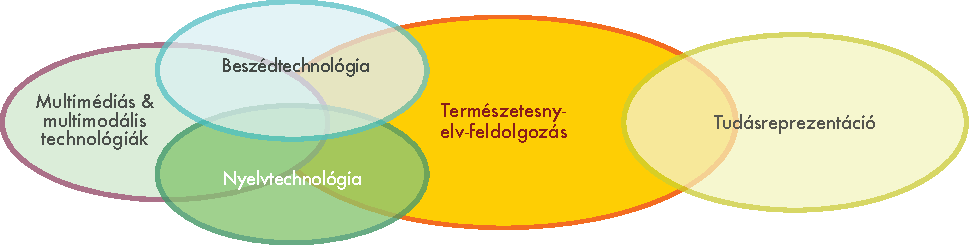
\includegraphics[width=\textwidth]{../_media/hungarian/language_technologies}
  \caption{Természetesnyelv-feldolgozás}
  \label{fig:ltincontext_de}
  \colorrule{grey3}{\textwidth}{1.5pt}
\end{figure*}

Kommunikációnkban ve\-gyít\-jük a nyelvet és a kommunikáció más módjait és csatornáit. A beszédet gesztusokkal és arckifejezésekkel kísérjük. A digitális szövegek képekkel és hangzó anyagokkal együtt jelennek meg. A filmek a nyelvet beszélt és írott formában is megjelenítik. Vagyis a beszéd- és nyelvtechnológia átfed és együttmőködik más technológiákkal, amelyek így együtt erősítik a multimodális kommunikáció és a multimédiás tartalmak feldolgozását. 

A következőkben a nyelvtechnológia fő alkalmazási területeit fogjuk tárgyalni, melyek a következők: nyelvi ellenőrzés, webes keresés, beszédtechnológia és gépi fordítás. Ezek olyan alkalmazásokat és technológiákat foglalnak magukban, mint például

\begin{itemize}
      \item helyesírás-ellenőrzés,
      \item szerzői támogatási rendszerek,
      \item gép által támogatott nyelvtanulás,
      \item információ-visszakeresés, 
      \item információkinyerés,
      \item szövegtömörítés,
      \item kérdésmegválaszoló rendszerek,
      \item beszédfelismerés és
      \item beszédszintézis.
    \end{itemize}

A nyelvtechnológia kiterjedt szakirodalommal rendelkezik, melyek közül az érdeklődő olvasót a következő olvasnivalókhoz irányítjuk: \cite{jurafsky-martin01} \cite{manning-schuetze1} \cite{lt-world1} \cite{lt-survey1}.

Mielőtt a fenti alkalmazási területeket tárgyalnánk, röviden bemutatjuk egy tipikus nyelvtechnológiai rendszer felépítését. 

\subsection{A nyelvtechnológiai alkalmazások felépítése}

A tipikus nyelvtechnológiai alkalmazások több komponensből állnak össze, amelyek a nyelv egyes szintjeit tükrözik. A \ref{fig:textprocessingarch_de}.~ábra egy szövegfeldolgozó rendszer egyszerűsített felépítését mutatja. Az első három modul a bemenő szöveg szerkezetét és jelentését dolgozza fel:

\begin{figure*}[htb]
  \colorrule{grey3}{\textwidth}{1.5pt}
  \center
  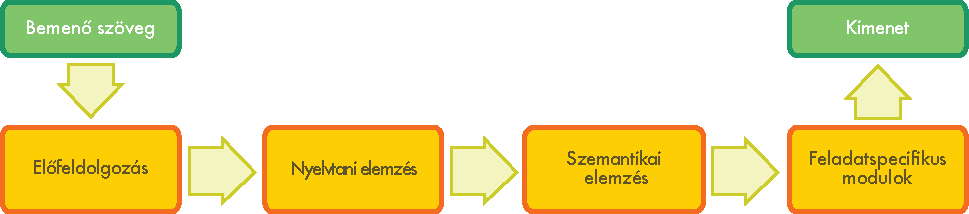
\includegraphics[width=\textwidth]{../_media/hungarian/text_processing_app_architecture}
  \caption{Egy tipikus szövegfeldolgozó alkalmazás felépítése}
  \label{fig:textprocessingarch_de}
  \colorrule{grey3}{\textwidth}{1.5pt}
\end{figure*}

\begin{enumerate}
      \item Előfeldolgozás: adattisztítás, a formázás eltávolítása, a bemenő szöveg nyelvének megállapítása, a speciális karakterek kezelése (pl. a magyar ékezetes betűk esetében) stb.
      \item Nyelvtani elemzés: az ige és argumentumainak megkeresése, a mondat szerkezetének feltárása.
      \item Szemantikai elemzés: egy\-ér\-tel\-mű\-sí\-tés (adott szónak az adott kontextusban mi a jelentése), az anaforák feloldása (a névmások kire/mire vonatkoznak), a mondat jelentésének reprezentálása valamilyen gép által olvasható formában. 
    \end{enumerate}

Ezután következnek a különféle feladatspecifikus modulok, mint például a bemenő szöveg automatikus tömörítése, az adatbázisokban való keresés és ehhez hasonlók. Mindez az alkalmazások fel\-épí\-té\-sé\-nek egyszerűsített és idealizált leírása, amely a nyelvtechnológiai alkalmazások komplexitását illusztrálja.  

A legfontosabb alkalmazási területek bemutatása után rövid kitekintésben beszámolunk a nyelvtechnológiai kutatási és oktatási helyzetről, különös tekintettel a már lezárult és a folyó kutatási prog\-ra\-mok\-ra. A fejezet végén szakértői értékelést adunk a legfontosabb nyelvtechnológiai esz\-kö\-zök\-ről és erőforrásokról olyan dimenziók mentén, mint az elérhetőség, a fejlettség és a minőség. A \pageref{fig:lrlttable_hu}.~oldalon található \ref{fig:lrlttable_hu}.~táblázat jó áttekintést ad a magyar nyelvtechnológia helyzetéről.

\subsection{A fő alkalmazási területek} 

Ebben a fejezetben a legfontosabb nyelv\-tech\-no\-ló\-giai eszközökre és erőforrásokra fókuszálunk, és áttekintést adunk a ma\-gyar\-or\-szá\-gi nyelvtechnológiai te\-vé\-keny\-ség\-ről. 

\subsubsection{Nyelvi ellenőrzés}

Mindenki, aki használt már a Microsoft Wordhöz hasonló szövegszerkesztőt, ta\-lál\-ko\-zott helyesírás-ellenőrző programmal, amely jelzi a helyesírási hibákat, és javítási javaslatokat tesz. Az első helyesírás-ellenőrző programok szimplán összehasonlították az ellenőrizendő szavakat a helyesen írt szavak listájával. A mai esz\-kö\-zök ennél sokkal kifinomultabbak. A szövegelemzéshez nyelvfüggő algoritmusokat használnak, amelyek a morfológiát (pl. a többes számú alakokat) is tudják kezelni, valamint a mondatszintű hibákat is detektálják, például ha hiányzik a ragozott ige a mondatból, vagy ha az ige és az alany nincsenek számban-személyben egyeztetve (pl.: \textit{én *írsz levelet}). Azonban a legtöbb nyelvi ellenőrző nem találna hibát a következő szövegben \cite{zar1}:

\begin{quote}
  I have a spelling checker,\\
  It came with my PC.\\
  It plane lee marks four my revue\\
  Miss steaks aye can knot sea.
\end{quote}

Az ilyen típusú hibák kezeléséhez az esetek nagy részében a kontextus elemzését is el kell végezni. A magyarban vannak olyan ragozott szavak, amelyek különböző jelentésekkel bírhatnak: például a \textit{várunk} lehet a \textit{vár} ige többes szám első személyű alakja, illetve a \textit{vár} főnév birtokos személyraggal ellátott alakja. 

A jelenség kezeléséhez nyelvspecifikus nyelvtani szabályok előállítására, vagyis magas szintű szakértői munkára, vagy pedig  statisztikai alapú nyelvmodellekre van szükség, amelyek alapján egy bizonyos szó adott környezetben való előfordulásának valószínűségét tudjuk kiszámolni. Például a \textit{várunk} valószínűleg nem ige, ha a mondatban már szerepel egy másik ragozott ige. Statisztikai alapú nyelvmodellek automatikusan előállíthatók nagy méretű, ellenőrzött adatot tartalmazó szöveghalmazokból, más néven korpuszokból. Ez a megközelítés elsősorban angol nyelvű adatokra lett kifejlesztve, de a magyarra is alkalmazható. Azt azonban figyelembe kell venni, hogy a módszerek nem ültethetők át egy az egyben a magyar nyelv agglutináló jellege és szabad szórendje miatt.

\boxtext{A nyelvi ellenőrzők használata nem csak a szövegszerkesztőkre korlátozódik, al\-kal\-maz\-zák még az ún.\ szerzői támogatási rendszerekben is.}

A nyelvi ellenőrzők használata nem csak a szövegszerkesztőkre korlátozódik, al\-kal\-maz\-zák még az ún.\ szerzői támogatási rendszerekben is, olyan szoftverkörnyezetekben, amelyekben használati utasításokat és egyéb dokumentációkat írnak speciális szten\-der\-dek alapján az információtechnológiai, az egészségügyi, a műszaki és egyéb termékek területén. A hibás vagy nehezen érthető használati útmutatók miatt bekövetkező károkról szóló vásárlói panaszoktól tartva a vállalatok egyre nagyobb hangsúlyt fektetnek a technikai dokumentáció minőségére, nemzetközi viszonylatokban is (fordítás, lokalizálás). A természetesnyelv-feldolgozás ered\-mé\-nyei a szerzői támogatási rendszerekben is fejlődést hoztak: a technikai dokumentáció szerzőit szótárak, terminológiai adatbázisok és mondattani szabályok segítik, melyek követik az adott terület előírásait.

\begin{figure*}[htb]
  \colorrule{grey3}{\textwidth}{1.5pt}
  \center
  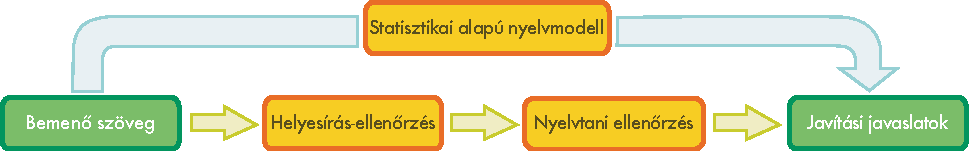
\includegraphics[width=\textwidth]{../_media/hungarian/language_checking}
  \caption{Nyelvi ellenőrzés (balra: szabályalapú, jobbra: statisztikai)}
  \label{fig:langcheckingaarch_de}
  \colorrule{grey3}{\textwidth}{1.5pt}
\end{figure*}

Tekintettel a magyar nyelv erősen agg\-lu\-ti\-ná\-ló jellegére, egy magyar nyelvű helyesírás-ellenőrzőnek tartalmaznia kell egy morfológiai elemző komponenst, hogy kezelni tudja a ragozott és összetett sza\-va\-kat is. Az első magyar helyesírás-ellenőrzőt a MorphoLogic Kft. \cite{morpho} fej\-lesz\-tet\-te ki a nyolcvanas években, amely egy helyesírás-ellenőrző modul és egy morfológiai modell kombinációjából állt elő. A \textit{Helyes-e?}\ programcsomag a Microsoft Office, a QuarkXPress, az Adobe InDesign és más szöveg- és ki\-ad\-vány\-szer\-kesz\-tő\-vel is használható. A MorphoLogic nyelvhelyesség-ellenőrző programokat is fejlesztett, amelyek felismernek olyan he\-lyes\-írá\-si hibákat, amelyeket a szóellenőrző programok nem tudnak megtalálni, mert a szöveget nem összefüggéseiben, hanem szavanként vizsgálják. A program nem feltétlenül hibákat jelez, hanem csak figyelmeztet. A jelzések nagy része tény\-le\-ges hibára utal, mások csak felhívják a figyelmet egy-egy lehetséges hibára. Az utóbbi esetben a felhasználónak kell eldöntenie, hogy tényleges hibáról van-e szó.

Nyílt forráskódú helyesírás-ellenőrző is létezik a magyarra. A Hunspell \cite{hunspell} a MySpellen alapul, és integrálva lett az OpenOffice-ba, a Mozilla Firefox 3-ba, a Mozilla Thunderbirdbe és a Google Chrome-ba.

A helyesírás-ellenőrzés és a szerzői támogatás mellett a nyelvi ellenőrzés a gép által támogatott nyelvtanulás terén is fontos szerepet tölt be, továbbá a webes keresőkben is alkalmazzák a lekérdezések automatikus javítására, például a Google keresési javaslatai esetében.

\subsubsection{Webes keresés}

A weben, intraneten vagy digitális könyv\-tá\-rak\-ban való keresés valószínűleg a leg\-töb\-bet használt és a legkevésbé fejlett nyelv\-tech\-no\-ló\-giai alkalmazás jelenleg. A Google kereső 1998-ban indult, és napjainkban a világ összes lekérdezésének 80\%-át végzi \cite{spi1}. Már a magyar nyelvben is elterjedt a \textit{guglizni} szó, bár a nyomtatott szótárakba még nem került bele. Sem a Google lekérdező felülete, sem a találati lista prezentációja nem változott jelentősen az első verzió óta. A jelenlegi változatban van viszont ellenőrző program, amely az elgépeléseket javítja, továbbá nemrég alapszintű szemantikai kereső alkalmazást építettek be, amely növeli a találati pontosságot azzal, hogy kontextusban vizsgálja a keresőkifejezést \cite{pc1}. A Google sikersztorija azt mutatja, hogy nagy mennyiségű adattal és hatékony indexelési technológiával a statisztikai alapú megközelítés kielégítő eredményt tud hozni. 

\begin{figure*}[htb]
  \colorrule{grey3}{\textwidth}{1.5pt}
  \center
  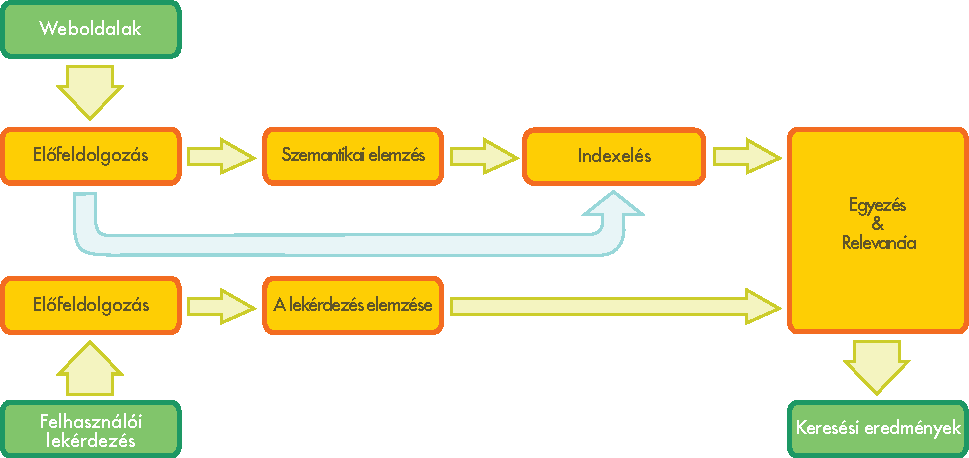
\includegraphics[width=\textwidth]{../_media/hungarian/web_search_architecture}
  \caption{A webes keresés architektúrája}
  \label{fig:websearcharch_de}
  \colorrule{grey3}{\textwidth}{1.5pt}
\end{figure*}

Azonban ha bonyolultabb információhoz akarunk jutni, mélyebb nyelvi tudásra van szükségünk a szövegértelmezéshez. Az olyan lexikai erőforrások, mint a gép által olvasható tezauruszok és a WordNethez hasonló ontológiák, javítják a keresés hatékonyságát azáltal, hogy a keresőkifejezés szinonimáit (pl. \textit{atomenergia, mag\-ener\-gia, nukleáris energia}) és a hozzá kapcsolódó szavakat is figyelembe veszik. 

A keresőmotorok új generációjának sokkal kifinomultabb nyelvtechnológiát kell al\-kal\-maz\-nia, különösen az olyan esetekben, amikor a keresés kérdést vagy más típusú mondatot tartalmaz, nem csak szavak listáját. Például képzeljünk el egy olyan lekérdezést, hogy ``Sorold fel azokat a cégeket, amelyeket az elmúlt öt évben vásároltak fel!''. A releváns válasz megtalálásához szükség van a mondat szintaktikai és szemantikai szintű elem\-zé\-sé\-re, valamint a releváns dokumentumok gyors elérését lehetővé tevő indexelésre is. A kielégítő válaszadáshoz a mondat teljes szintaktikai elemzését el kell végezni, és rá kell jönni, hogy a felhasználó azokra a cégekre kíváncsi, amelyeket felvásároltak, és nem azokra, amelyek felvásároltak cégeket. Ezen felül az időt jelölő kifejezést is fel kell dolgozni ahhoz, hogy kiderüljön, hogy mely évekről van szó. Végül a feldolgozott keresőkifejezést össze kell vetni nagy mennyiségű strukturálatlan adattal, hogy megtaláljuk azt az információt, amelyet a felhasználó keres. Ezt, vagyis a keresést és a releváns találatok sorrendezését hívják információ-visszakeresésnek. Továbbá ahhoz, hogy cégek listáját kapjuk, ki kell nyernünk azt az információt a dokumentumokból, hogy szavak egy adott sorozata egy cégre utal. Ezt a fajta információkinyerést végzik az automatikus tulajdonnév-felismerők.  

\boxtext{A keresőmotorok új generációjának sokkal kifinomultabb nyelvtechnológiát kell al\-kal\-maz\-nia.}

Még több nyelvtechnológiát igényel egy keresőkifejezés megtalálása más nyelvű dokumentumokban. A nyelvközi in\-for\-má\-ció-visszakereséshez először le kell fordítani a keresőkifejezést az összes lehetséges forrásnyelvre, majd a találatokat vissza kell fordítani a célnyelvre. 

A nem szöveges formában levő adatok növekvő aránya hívta életre az igényt a multimédiás információ-visszakereső szolgáltatásokra, vagyis a képekben, hangzó anyagokban, videókban való keresésre. Az audió- és videófájlok esetében szükség van egy beszédfelismerő modulra is, amely a beszédet szöveggé alakítja át, amelyben így már lehet keresni.

Mivel a magyar nem olyan kötött szórendő, mint például az angol, a magyar mondatelemzők fejlesztése során nem tudunk pusztán a mondat lineáris szerkezetére támaszkodni. Viszont az esetragok és névutók fogódzót jelentenek, mivel ezek határozzák meg a mondatrészek szerepét. Az igék és a hozzájuk tartozó vonzatok alkotják a mondat szerkezetének alapját, ezért fontosak az ún.\ vonzatkerettárak. Egy ilyen adatbázist fejlesztettek az MTA Nyelvtudományi Intézetének munkatársai, amely magasabb szintű elemző alkalmazásokba, például szabályalapú szintaktikai elem\-ző\-be is beépíthető. Ez utóbbiból több is létezik a magyarra -- egyik a Szeged Treebankbe, egy másik pedig a MetaMorpho nevő szabályalapú gépi fordítóba lett beépítve. 

A nyelvtechnológiával foglalkozó cégek és kutatóműhelyek fő kutatási irányai között szerepel olyan trend- és szövegelemző esz\-kö\-zök fejlesztése, amelyek ter\-mé\-sze\-tes\-nyelv-feldolgozó alkalmazásokat integrálnak annak érdekében, hogy a strukturálatlan szövegben megtalálják a releváns információkat. Erre a célra magyar nyelvű morfológiai elemzők és egyértelmősítők, valamint tulajdonnév-felismerők állnak rendelkezésre, melyek nagyrészt statisztikai tanuló algoritmusokon alapulnak.

Létezik egy magyar nyelvű általános célú metakereső, a PolyMeta \cite{polymeta}, amely le\-he\-tő\-sé\-get nyújt tetszőleges számú, interneten keresztül elérhető adatbázis, forrás egyidejű lekérdezésére. A találati eredményekből közös lista készül, amelyben az elemek fontossági sorrend szerint vannak rendezve. A metakereső természetesnyelv-feldolgozási és információ-visszakeresési algoritmusokat használ a keresőkifejezések elemzéséhez és a találatok sorrendezéséhez.

De nemcsak kis- és középvállalatok fej\-lesz\-te\-nek információkinyerő eszközöket Magyarországon. Számos olyan projekt fut különböző egyetemeken és kutatóintézetekben, melyek célja szemantikai alapú keresőrendszerek fejlesztése, vagy magyar nyelvű ontológiák (pl. Ma\-gyar WordNet, Magyar Egységes Ontológia) építése. 
  
\subsubsection{Beszédtechnológia}

A beszédtechnológia szolgáltatja az alapot olyan interfészek előállításához, amelyek lehetővé teszik, hogy a felhasználók a gépekkel természetes emberi nyelven, és ne csak grafikus felület, billentyűzet vagy egér segítségével kommunikáljanak. Napjainkban ilyen beszédinterfészeket al\-kal\-maz\-nak bizonyos szolgáltatások részleges vagy teljes automatizálására. Az üzleti szférában elsősorban a bankok, a logisztikával, a szállítással és a telekommunikációval foglalkozó cégek használják. A beszédtechnológiát alkalmazzák még autós navigációs rendszerekben és az okostelefonokban a grafikus felület alternatívájaként.

\boxtext{A beszédtechnológia szolgáltatja az alapot olyan interfészek előállításához, amelyek lehetővé teszik, hogy a felhasználók a gépekkel természetes emberi nyelven, és ne csak grafikus felület, billentyűzet vagy egér segítségével kommunikáljanak.}

\begin{figure*}[htb]
  \colorrule{grey3}{\textwidth}{1.5pt}
  \center 
  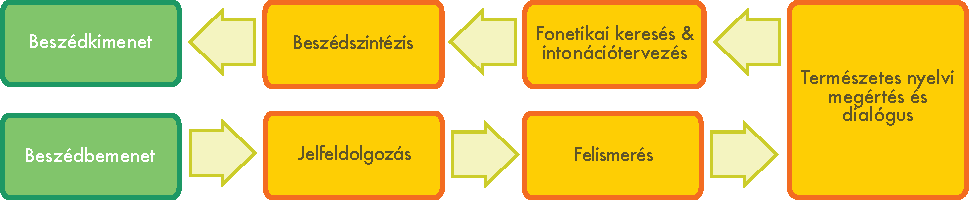
\includegraphics[width=\textwidth]{../_media/hungarian/simple_speech-based_dialogue_architecture}
  \caption{Egyszerű beszédalapú dialógus felépítése}
  \label{fig:dialoguearch_de}
  \colorrule{grey3}{\textwidth}{1.5pt}
\end{figure*}

A beszédtechnológia az alábbi négy fő technológiai területet foglalja magában:

\begin{enumerate}
      \item Az automatikus beszédfelismerés határozza meg, hogy mely szavakat mondta ki a felhasználó.
      \item A szintaktikai elemzés és a szemantikai interpretáció segítségével ele\-mez\-he\-tő a felhasználó közlésének szintaktikai szerkezete, valamint leképezhető annak szemantikai interpretációja az adott rendszer céljainak megfelelően. 
      \item A dialógusvezérlés az input nyelvi jellemzői, az adott felhasználó és feladat egyéni beállításai alapján valósítja meg a rendszer megfelelő lépését, az adatbázis-lekérdezést.     
      \item A beszédszintézis technológiáját alkalmazzák arra, hogy a gép előállítsa a megfelelő beszédkimenetet. 
    \end{enumerate}

Az egyik legnagyobb kihívást az automatikus beszédfelismerés jelenti, vagyis hogy a rendszer minél pontosabban felismerje a felhasználó által kiejtett szavakat. Ez kétféleképpen történhet: vagy a felhasználó által használható kifejezéseket csökkentjük kulcsszavak egy limitált nagy\-sá\-gú halmazára, vagy nyelvmodelleket állítunk elő, amelyek a természetes nyelvi kifejezések egy nagyobb hányadát fedik le. A gépi tanulási technikákat használva nyelvmodelleket állíthatunk elő auto\-ma\-ti\-ku\-san szövegkorpuszokból, vagyis audiófájlok és szöveges átirataik nagyméretű gyűjteményéből. Míg a kulcsszavas módszer merev és nehezen használható beszédinterfészt, valamint kevésbé elfogadható kimenetet eredményez, addig a nyelv\-mo\-del\-lek előállítása és finomhangolása a költségeket emeli meg erőteljesen. Azonban a nyelvmodelleket alkalmazó beszédinterfész nagyobb elfogadottsággal rendelkezik a felhasználók körében, és előnyösebb, mint a kevésbé rugalmas rendszervezérelt megközelítés. 

Ami a beszédinterfész kimeneti oldalát illeti, a vállalatok egyre inkább előre felvett kifejezéseket használnak. A statikus kifejezések esetében, amikor a beszéd nem függ adott kontextustól vagy a felhasználó adataitól, ez a módszer kellő mértékű felhasználói elégedettséget eredményez. Viszont minél dinamikusabb a lejátszani kívánt tartalom, annál rosszabb lesz az ele\-mek\-ből összeállított mondat prozódiája az audiófájlok összevágása miatt -- még akkor is, ha a mai beszédszintetizáló rendszerek egyre jobban teljesítenek, köszönhetően az egyre természetesebbé váló prozódiának. 

A beszédtechnológia piacán az elmúlt évtizedekben fontos szabványosítási lépések történtek a különböző technológiai komponensek közötti interfészek, valamint az egyes alkalmazásokra épülő termékek ese\-té\-ben is. Intenzív piaci konszolidáció zajlott le az elmúlt tíz évben, főként a beszédfelismerés és -szintézis terén. A G20 országok nemzeti piacait kevesebb mint 5 cég dominálja, mint a Nuance (USA) és a Loquendo (Olaszország), csak hogy a legprominensebbeket említsük az európai piacról. 2011-ben a Nuance bejelentette, hogy felvásárolja a Loquendót, ami egy újabb lépés a piac konszolidációja felé. 

A magyar nyelv speciális jellege miatt a világszerte széles körben alkalmazott módszerek vagy egyáltalán nem, vagy csak nehezen adaptálhatók a magyarra. Vi\-szont a kifejezetten a magyarra ki\-fej\-lesz\-tett módszerek könnyen alkalmazhatók lehetnek a hasonlóan agglutináló nyel\-vek\-re, mint a finnre, a törökre vagy az arabra. 

A magyar beszédszintézis piacát a Budapesti Műszaki és Gazdaságtudományi Egyetemen (BME) dolgozó kutatócsoportok \cite{bme} dominálják. A legszélesebb körben használt magyar beszédszintetizátor a Profivox, amely 2002 óta elérhető, és amelyet több alkalmazásba is beépítettek: SMS- és e-mailfelolvasó szoftverbe, autós és mobiltelefonos GPS rendszerbe, valamint e-book- és képernyőolvasó szolgáltatásba, amelyek segíthetik a látássérült emberek integrációját az információs társadalomba. Egy magas szinten vezérelhető interaktív fejlesztői környezet is rendelkezésre áll speciális kutatási célok támogatására (pl. pszichológiai és prozódiai vizsgálatokra). A szoftver szövegfelolvasó (TTS) technológián alapul. Segítségével meghatározott akusztikai és prozódiai tartalommal bíró kísérleti jel hozható létre kont\-rol\-lál\-ha\-tó körülmények között. Egy 1,5 millió szóalakot tartalmazó magyar kiejtési szótár is elérhető. Ennek alapján ki\-ala\-kít\-ha\-tó egy magyar szövegeket (fonetikai) szimbólumokká alakító eszköz. 

Beszédfelismeréssel Magyarországon a fentebb említett és más egyetemi ku\-ta\-tó\-mű\-he\-lyek (pl. a Szegedi Tu\-do\-mány\-egye\-tem Informatikai Tanszékcsoportja) mellett kisebb vállalkozások is foglalkoznak, mint az Alkalmazott Logikai La\-bo\-ra\-tó\-ri\-um, az Aitia vagy a Digital Natives Kft. A már említett nyelvi nehézségek ellenére több magyar nyelvű gépi beszédfelismerő alkalmazást is kifejlesztettek az elmúlt években. A BME Távközlési és Mé\-dia\-in\-for\-ma\-ti\-kai Tanszékén kifejlesztettek egy statisztikai alapú folyamatosbeszéd-felismerő motort és fejlesztői környezetet, továbbá egy kötött hangsúlyozáson alapuló szóhatár-detektáló alkalmazást ma\-gyar és finn nyelvekre, melyet egy nyelv\-kö\-zi vizsgálat előzött meg. A már említett kutatóműhelyek közös munkájának eredményeképpen különféle orvosi leletező beszédfelismerők is készültek, melyek az orvosi vizsgálatokat közvetlen beszéd-szöveg átalakítással segítik. Továbbá létezik egy olyan alkalmazás, amely a beszédhibás gyerekek beszédtanulását se\-gí\-ti, és a magyar mellett több más európai nyelven is használható. A beszédfelismerő rendszerek számos további gyakorlati alkalmazást segíthetnek. Ilyen például a telefonos hívások kezelése vagy a te\-le\-fon\-köz\-pont-irányítás.

A jövőben jelentős változásokat fog hozni az ügyfélkapcsolatok kezelésében a ha\-gyo\-má\-nyos telefon, az internet és az e-mail mellett az okostelefonok terjedése, ami hatással lesz a beszédtechnológiára is. Hosszútávon kevesebb telefonalapú felhasználói interfész lesz, és a beszélt nyelv mint felhasználóbarát bemenet sokkal inkább központi szerepet fog játszani. Ez nagyrészt annak köszönhető, hogy a beszélőfüggetlen beszédfelismerés pontosságának javításában előrelépések tör\-tén\-tek azáltal, hogy a diktáló rend\-sze\-rek már most beépített szolgáltatások az okostelefon-használók számára.

\subsubsection{Gépi fordítás}

A digitális számítógépek alkalmazásának ötlete természetes nyelvek lefordítására 1946-ban merült fel először. Az ötletet az ötvenes években anyagi támogatás is követte, ami azonban csak a nyolcvanas években folytatódott. Mindemellett a gépi fordítás még mindig nem váltotta be a kezdeti nagy reményeket.

\boxtext{A legalacsonyabb szinten a gépi fordítás egyszerű behelyettesítés: az egyik természetes nyelvű szót lecseréljük egy másik nyelvű szóra.}

A legalacsonyabb szinten a gépi fordítás egyszerű behelyettesítés: az egyik természetes nyelvű szót lecseréljük egy másik nyelvű szóra. Ez az eljárás csak nagyon szűk szókincsű, formalizált nyelvű szö\-ve\-gek (pl. időjárás-jelentések) esetében működik. A kevésbé kötött szövegek jó fordításához nagyobb szö\-veg\-egy\-sé\-ge\-ket (frá\-zi\-so\-kat, mon\-da\-to\-kat vagy teljes bekezdéseket) kell illeszteni a másik nyelvű megfelelőikhez. A legfőbb problémát az okozza, hogy az emberi nyelv sokszor többértelmű, ami minden szinten kihívások elé állítja a nyelvfeldolgozókat. A lexikai szinten a szójelentés-egyértelműsítés (pl.\ a \textit{nyúl} lehet cselekvés és állat is), míg a mondat szintjén akár az esetragos főnévi csoportok is okozhatnak nehézségeket, mint ezekben a mondatokban:

\begin{itemize}
\item A rendőr látta az embert a távcsővel. 
\item A rendőr látta az embert a revolverrel.
\end{itemize}

A feladat egyik megközelítési módja nyelvtani szabályokon alapul. Közeli rokon nyelvek esetében a közvetlen fordítás kivitelezhető lehet a fenti példákra is. De általában a szabályalapú (vagy tu\-dás\-ve\-zé\-relt) rendszerek úgy működnek, hogy először elemzik a bemenő szöveget, majd egy közvetítő, szimbolikus reprezentációt alkotnak, és ez utóbbiból generálják a célnyelvi kimenetet. Ezeknek a rend\-sze\-rek\-nek a teljesítménye morfológiai, szintaktikai és szemantikai információt egyaránt tartalmazó lexikonok, valamint nyelvész szakértők által aprólékosan kidolgozott nyelvtani szabályok meglététől egyaránt erősen függ, amelyek előállítása hosszú és költséges folyamat.

\begin{figure*}[htb]
  \colorrule{grey3}{\textwidth}{1.5pt}
  \center
  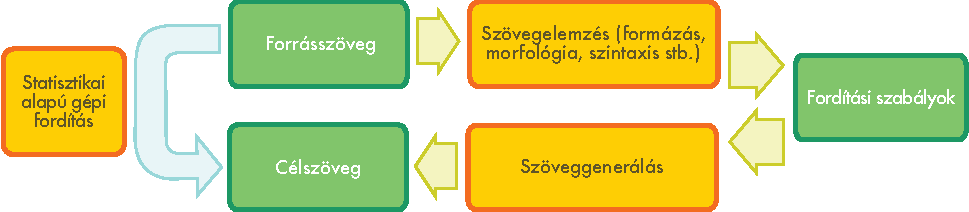
\includegraphics[width=\textwidth]{../_media/hungarian/machine_translation}
  \caption{Gépi fordítás (fent: statisztikai, lent: szabályalapú)}
  \label{fig:mtarch_de}
  \colorrule{grey3}{\textwidth}{1.5pt}
\end{figure*}

A nyolcvanas évek végétől kezdve, ahogy a számítógépek egyre olcsóbbak lettek, és teljesítményük nőtt, egyre nagyobb érdeklődés mutatkozott a statisztikai modellek iránt a gépi fordítás terén. Ezeknek a statisztikai modelleknek a paramétereit párhuzamos korpuszokból lehet kiszámítani, mint amilyen az Europarl pár\-hu\-za\-mos korpusz, amely az Európai Parlament jegyzőkönyveit tartalmazza 11 európai nyelven. Kellő mennyiségű adat birtokában a statisztikai alapú gépi fordítás elég jó becslést tud adni egy idegen nyelvű szöveg jelentéséről. Azonban a szabályalapú rendszerekkel ellentétben a statisztikai (más néven adatvezérelt) gépi fordítók gyakran nyelvtanilag helytelen kimenetet produkálnak. Másrészről vi\-szont az adatvezérelt rendszereknek több előnyük is van: amellett, hogy kevesebb emberi munkát igényelnek, a nyelv olyan különlegességeit is tudják kezelni (például az idiomatikus kifejezéseket), amilyeneket a szabályalapúak nem. 

Mivel a szabályalapú és a statisztikai alapú módszerek erősségei és gyengeségei kiegészítik egymást, a kutatók manapság már inkább a két megközelítést ötvöző hib\-rid rendszereken dolgoznak. Ezt több\-fé\-le\-kép\-pen lehet megvalósítani. Az egyik út, amikor mindkét módszert használjuk, és minden mondatra kiválasztjuk a legjobb kimenetet. Ennél jobb megoldást ad, ha a különböző kimenetekből összeválogatjuk a legjobb mondatrészeket, ami meglehetősen komplex feladat lehet, hiszen nincs mindig egyértelmű megfelelés a mondatrészek között.  

\boxtext{A gépi fordítás a magyar nyelvre különösen nehéz.} 

A gépi fordítás a magyar nyelvre különösen nehéz. A szabad szórend és az elváló igekötők problémát okoznak az elemzés során, a gazdag ragozási rendszer pedig kihívásokat jelent a megfelelő esetraggal rendelkező szóalakok előállításánál.

A nehézségek ellenére a gépi fordítás ma\-gyar piacán is léteznek szabályalapú és adatvezérelt megoldások. A MorphoLogic Kft.\ számítógépes gépi fordító prog\-ram\-cso\-ma\-go\-kat és online fordító szolgáltatást egyaránt kínál. A MorphoWord angol és magyar nyelv között fordít, mindkét irányba. Rendszerük szabályalapú és statisztikai módszereket ötvöz, de a fő komponens a fordítandó szöveghez egy belső reprezentációt rendel, majd ezt alakítja célnyelvű szöveggé. 

A nagyméretű kétnyelvű szövegek kulcsfontosságúak a statisztikai alapú gépi fordításhoz. A Hunglish korpusz szabadon elérhető, mondatszinten párhuzamosított magyar-angol párhuzamos korpusz, amely 2,07 millió mondatban 54,2 millió szót tartalmaz. Jelenleg ez a legnagyobb magyar-angol párhuzamos korpusz. A mondatok illesztése a hunalign nevű esz\-köz\-zel történt, amelyet a BME kutatói fej\-lesz\-tet\-tek ki, és az egyik leggyakrabban használt mondatszintű il\-lesz\-tő\-prog\-ram. A Hunglish mondattár egy online felületen keresztül elérhető és lekérdezhető \cite{hunglish}, így nyersfordítóként vagy kétnyelvű szótárként is használható.

2010 márciusában indult az iTranslate4.eu \cite{it4eu} projekt, melynek célja olyan gépi fordító szolgáltatás nyújtása, amely nemcsak lefedi az Európai Unió összes nyelvét, hanem az összes nyelvpár esetében a mindenkori legjobb minőségű fordítást is adja. Ezt a tervet az Európa legjobb gépifordító-rendszereinek működtetői által létrehozott konzorcium valósítja meg, amelynek tagjai legalább egy nyelvpár legjobb fordítását biztosítják. A projektnek két magyar résztvevője is van: a konzorciumvezető az MTA Nyelvtudományi Intézete, míg a szolgáltatások közös interfészét a MorphoLogic Kft.\ nyújtja. 

A gépi fordítás nagy mértékben tudja javítani a hatékonyságot, főként ha intelligensen igazítható a felhasználóspecifikus terminológiához, illetve integrálható a megfelelő munkakörnyezetbe. A ma\-gyar nyelvre is léteznek ilyen interaktív fordítástámogató rendszerek, például a Kilgray Kft.\ által fejlesztett memoQ prog\-ram\-cso\-mag \cite{memoq}. 

Még mindig nagy potenciál rejlik a gépi fordító rendszerek minőségének ja\-ví\-tá\-sá\-ban, például a nyelvi erőforrások egy adott felhasználói területre való alkalmazásával, vagy a terminológiai adatbázisok és a fordítómemóriák esetében alkalmazott munkakörnyezetek integrálásával. Problémát jelent, hogy a jelenlegi rendszerek nagy része angolközpontú, és a magyarról és magyarra való fordítás is csak angolra, illetve angolról működik. Ez fennakadásokat okoz a fordítói munkafolyamatban, és arra kényszeríti a gépi fordítást használókat, hogy különböző rendszerek különböző lexikai eszközeinek használatát is elsajátítsák.

A gépi fordító rendszerek, a különböző módszerek és a különböző nyelvpárokra működő rendszerek összehasonlítását ki\-ér\-té\-ke\-lő kampányok segítik. A \ref{fig:euromatrix_hu}.~táblázat, amely az Európai Bizottság Euromatrix+ projektje keretében készült, a nyelvpárokra lebontott teljesítményt mutatja a 23 hivatalos európai nyelv közül 22-re (az ír nyelv nem szerepel az összehasonlításban). Az eredményeket a BLEU-érték \cite{bleu1} alapján rangsorolták, amely szerint a jobb fordítás magasabb pontszámot kap. Az emberi fordítás kb. 80 pontot kapna.

A legjobb eredmények (zölddel és kékkel jelölve) azon nyelvek esetében születtek, amelyek koordinált programokban vettek részt, és amelyekre kellő mennyiségű párhuzamos korpusz áll rendelkezésre (pl. angol, francia, holland, spanyol és német). A gyengébb eredményt elért nyelvek pi\-ros\-sal kiemelve láthatók. Ezek vagy nélkülözni voltak kénytelenek a kutatási ráfordításokat, vagy strukturálisan különböznek a többi nyelvtől (pl. magyar, máltai és finn).

\begin{figure*}[htbp]
  \centering
  \setlength{\tabcolsep}{0.17em}
  \small
  \begin{tabular}{>{\columncolor{corange1}}cccccccccccccccccccccccc}
    & \multicolumn{22}{>{\columncolor{corange1}}c}{Célnyelv -- \textcolor{grey1}{Target language}}\\\addlinespace[{-.009cm}]
    \rowcolor{corange1}  & EN & BG & DE & CS & DA & EL & ES & ET & FI & FR & HU & IT & LT & LV & MT & NL & PL & PT & RO & SK & SL & SV\\
    EN & -- & \textcolor{blue}{40.5} & \textcolor{blue}{46.8} & \textcolor{green2}{52.6} & \textcolor{green2}{50.0} & \textcolor{blue}{41.0} & \textcolor{green2}{55.2} & \textcolor{purple}{34.8} & \textcolor{purple}{38.6} & \textcolor{green2}{50.1} & \textcolor{purple}{37.2} & \textcolor{green2}{50.4} & \textcolor{purple}{39.6} & \textcolor{blue}{43.4} & \textcolor{purple}{39.8} & \textcolor{green2}{52.3} & \textcolor{blue}{49.2} & \textcolor{green2}{55.0} & \textcolor{blue}{49.0} & \textcolor{blue}{44.7} & \textcolor{green2}{50.7} & \textcolor{green2}{52.0}\\
    BG & \textcolor{green}{61.3} & -- & \textcolor{purple}{38.7} & \textcolor{purple}{39.4} & \textcolor{purple}{39.6} & \textcolor{purple}{34.5} & \textcolor{blue}{46.9} & \textcolor{red3}{25.5} & \textcolor{red3}{26.7} & \textcolor{blue}{42.4} & \textcolor{red3}{22.0} & \textcolor{blue}{43.5} & \textcolor{red3}{29.3} & \textcolor{red3}{29.1} & \textcolor{red3}{25.9} & \textcolor{blue}{44.9} & \textcolor{purple}{35.1} & \textcolor{blue}{45.9} & \textcolor{purple}{36.8} & \textcolor{purple}{34.1} & \textcolor{purple}{34.1} & \textcolor{purple}{39.9}\\
    DE & \textcolor{green2}{53.6} & \textcolor{red3}{26.3} & -- & \textcolor{purple}{35.4} & \textcolor{blue}{43.1} & \textcolor{purple}{32.8} & \textcolor{blue}{47.1} & \textcolor{red3}{26.7} & \textcolor{red3}{29.5} & \textcolor{purple}{39.4} & \textcolor{red3}{27.6} & \textcolor{blue}{42.7} & \textcolor{red3}{27.6} & \textcolor{purple}{30.3} & \textcolor{red2}{19.8} & \textcolor{green2}{50.2} & \textcolor{purple}{30.2} & \textcolor{blue}{44.1} & \textcolor{purple}{30.7} & \textcolor{red3}{29.4} & \textcolor{purple}{31.4} & \textcolor{blue}{41.2}\\
    CS & \textcolor{green2}{58.4} & \textcolor{purple}{32.0} & \textcolor{blue}{42.6} & -- & \textcolor{blue}{43.6} & \textcolor{purple}{34.6} & \textcolor{blue}{48.9} & \textcolor{purple}{30.7} & \textcolor{purple}{30.5} & \textcolor{blue}{41.6} & \textcolor{red3}{27.4} & \textcolor{blue}{44.3} & \textcolor{purple}{34.5} & \textcolor{purple}{35.8} & \textcolor{red3}{26.3} & \textcolor{blue}{46.5} & \textcolor{purple}{39.2} & \textcolor{blue}{45.7} & \textcolor{purple}{36.5} & \textcolor{blue}{43.6} & \textcolor{blue}{41.3} & \textcolor{blue}{42.9}\\
    DA & \textcolor{green2}{57.6} & \textcolor{red3}{28.7} & \textcolor{blue}{44.1} & \textcolor{purple}{35.7} & -- & \textcolor{purple}{34.3} & \textcolor{blue}{47.5} & \textcolor{red3}{27.8} & \textcolor{purple}{31.6} & \textcolor{blue}{41.3} & \textcolor{red3}{24.2} & \textcolor{blue}{43.8} & \textcolor{red3}{29.7} & \textcolor{purple}{32.9} & \textcolor{red3}{21.1} & \textcolor{blue}{48.5} & \textcolor{purple}{34.3} & \textcolor{blue}{45.4} & \textcolor{purple}{33.9} & \textcolor{purple}{33.0} & \textcolor{purple}{36.2} & \textcolor{blue}{47.2}\\
    EL & \textcolor{green2}{59.5} & \textcolor{purple}{32.4} & \textcolor{blue}{43.1} & \textcolor{purple}{37.7} & \textcolor{blue}{44.5} & -- & \textcolor{green2}{54.0} & \textcolor{red3}{26.5} & \textcolor{red3}{29.0} & \textcolor{blue}{48.3} & \textcolor{red3}{23.7} & \textcolor{blue}{49.6} & \textcolor{red3}{29.0} & \textcolor{purple}{32.6} & \textcolor{red3}{23.8} & \textcolor{blue}{48.9} & \textcolor{purple}{34.2} & \textcolor{green2}{52.5} & \textcolor{purple}{37.2} & \textcolor{purple}{33.1} & \textcolor{purple}{36.3} & \textcolor{blue}{43.3}\\
    ES & \textcolor{green}{60.0} & \textcolor{purple}{31.1} & \textcolor{blue}{42.7} & \textcolor{purple}{37.5} & \textcolor{blue}{44.4} & \textcolor{purple}{39.4} & -- & \textcolor{red3}{25.4} & \textcolor{red3}{28.5} & \textcolor{green2}{51.3} & \textcolor{red3}{24.0} & \textcolor{green2}{51.7} & \textcolor{red3}{26.8} & \textcolor{purple}{30.5} & \textcolor{red3}{24.6} & \textcolor{blue}{48.8} & \textcolor{purple}{33.9} & \textcolor{green2}{57.3} & \textcolor{purple}{38.1} & \textcolor{purple}{31.7} & \textcolor{purple}{33.9} & \textcolor{blue}{43.7}\\
    ET & \textcolor{green2}{52.0} & \textcolor{red3}{24.6} & \textcolor{purple}{37.3} & \textcolor{purple}{35.2} & \textcolor{purple}{37.8} & \textcolor{red3}{28.2} & \textcolor{blue}{40.4} & -- & \textcolor{purple}{37.7} & \textcolor{purple}{33.4} & \textcolor{purple}{30.9} & \textcolor{purple}{37.0} & \textcolor{purple}{35.0} & \textcolor{purple}{36.9} & \textcolor{red3}{20.5} & \textcolor{blue}{41.3} & \textcolor{purple}{32.0} & \textcolor{purple}{37.8} & \textcolor{red3}{28.0} & \textcolor{purple}{30.6} & \textcolor{purple}{32.9} & \textcolor{purple}{37.3}\\
    FI & \textcolor{blue}{49.3} & \textcolor{red3}{23.2} & \textcolor{purple}{36.0} & \textcolor{purple}{32.0} & \textcolor{purple}{37.9} & \textcolor{red3}{27.2} & \textcolor{purple}{39.7} & \textcolor{purple}{34.9} & -- & \textcolor{red3}{29.5} & \textcolor{red3}{27.2} & \textcolor{purple}{36.6} & \textcolor{purple}{30.5} & \textcolor{purple}{32.5} & \textcolor{red2}{19.4} & \textcolor{blue}{40.6} & \textcolor{red3}{28.8} & \textcolor{purple}{37.5} & \textcolor{red3}{26.5} & \textcolor{red3}{27.3} & \textcolor{red3}{28.2} & \textcolor{purple}{37.6}\\
    FR & \textcolor{green}{64.0} & \textcolor{purple}{34.5} & \textcolor{blue}{45.1} & \textcolor{purple}{39.5} & \textcolor{blue}{47.4} & \textcolor{blue}{42.8} & \textcolor{green}{60.9} & \textcolor{red3}{26.7} & \textcolor{purple}{30.0} & -- & \textcolor{red3}{25.5} & \textcolor{green2}{56.1} & \textcolor{red3}{28.3} & \textcolor{purple}{31.9} & \textcolor{red3}{25.3} & \textcolor{green2}{51.6} & \textcolor{purple}{35.7} & \textcolor{green}{61.0} & \textcolor{blue}{43.8} & \textcolor{purple}{33.1} & \textcolor{purple}{35.6} & \textcolor{blue}{45.8}\\
    HU & \textcolor{blue}{48.0} & \textcolor{red3}{24.7} & \textcolor{purple}{34.3} & \textcolor{purple}{30.0} & \textcolor{purple}{33.0} & \textcolor{red3}{25.5} & \textcolor{purple}{34.1} & \textcolor{red3}{29.6} & \textcolor{red3}{29.4} & \textcolor{purple}{30.7} & -- & \textcolor{purple}{33.5} & \textcolor{red3}{29.6} & \textcolor{purple}{31.9} & \textcolor{red2}{18.1} & \textcolor{purple}{36.1} & \textcolor{red3}{29.8} & \textcolor{purple}{34.2} & \textcolor{red3}{25.7} & \textcolor{red3}{25.6} & \textcolor{red3}{28.2} & \textcolor{purple}{30.5}\\
    IT & \textcolor{green}{61.0} & \textcolor{purple}{32.1} & \textcolor{blue}{44.3} & \textcolor{purple}{38.9} & \textcolor{blue}{45.8} & \textcolor{blue}{40.6} & \textcolor{red3}{26.9} & \textcolor{red3}{25.0} & \textcolor{red3}{29.7} & \textcolor{green2}{52.7} & \textcolor{red3}{24.2} & -- & \textcolor{red3}{29.4} & \textcolor{purple}{32.6} & \textcolor{red3}{24.6} & \textcolor{green2}{50.5} & \textcolor{purple}{35.2} & \textcolor{green2}{56.5} & \textcolor{purple}{39.3} & \textcolor{purple}{32.5} & \textcolor{purple}{34.7} & \textcolor{blue}{44.3}\\
    LT & \textcolor{green2}{51.8} & \textcolor{red3}{27.6} & \textcolor{purple}{33.9} & \textcolor{purple}{37.0} & \textcolor{purple}{36.8} & \textcolor{red3}{26.5} & \textcolor{red3}{21.1} & \textcolor{purple}{34.2} & \textcolor{purple}{32.0} & \textcolor{purple}{34.4} & \textcolor{red3}{28.5} & \textcolor{purple}{36.8} & -- & \textcolor{blue}{40.1} & \textcolor{red3}{22.2} & \textcolor{purple}{38.1} & \textcolor{purple}{31.6} & \textcolor{purple}{31.6} & \textcolor{red3}{29.3} & \textcolor{purple}{31.8} & \textcolor{purple}{35.3} & \textcolor{purple}{35.3}\\
    LV & \textcolor{green2}{54.0} & \textcolor{red3}{29.1} & \textcolor{purple}{35.0} & \textcolor{purple}{37.8} & \textcolor{purple}{38.5} & \textcolor{red3}{29.7} & \textcolor{red2}{8.0} & \textcolor{purple}{34.2} & \textcolor{purple}{32.4} & \textcolor{purple}{35.6} & \textcolor{red3}{29.3} & \textcolor{purple}{38.9} & \textcolor{purple}{38.4} & -- & \textcolor{red3}{23.3} & \textcolor{blue}{41.5} & \textcolor{purple}{34.4} & \textcolor{purple}{39.6} & \textcolor{purple}{31.0} & \textcolor{purple}{33.3} & \textcolor{purple}{37.1} & \textcolor{purple}{38.0}\\
    MT & \textcolor{green}{72.1} & \textcolor{purple}{32.2} & \textcolor{purple}{37.2} & \textcolor{purple}{37.9} & \textcolor{purple}{38.9} & \textcolor{purple}{33.7} & \textcolor{blue}{48.7} & \textcolor{red3}{26.9} & \textcolor{red3}{25.8} & \textcolor{blue}{42.4} & \textcolor{red3}{22.4} & \textcolor{blue}{43.7} & \textcolor{purple}{30.2} & \textcolor{purple}{33.2} & -- & \textcolor{blue}{44.0} & \textcolor{purple}{37.1} & \textcolor{blue}{45.9} & \textcolor{purple}{38.9} & \textcolor{purple}{35.8} & \textcolor{blue}{40.0} & \textcolor{blue}{41.6}\\
    NL & \textcolor{green2}{56.9} & \textcolor{red3}{29.3} & \textcolor{blue}{46.9} & \textcolor{purple}{37.0} & \textcolor{blue}{45.4} & \textcolor{purple}{35.3} & \textcolor{blue}{49.7} & \textcolor{red3}{27.5} & \textcolor{red3}{29.8} & \textcolor{blue}{43.4} & \textcolor{red3}{25.3} & \textcolor{blue}{44.5} & \textcolor{red3}{28.6} & \textcolor{purple}{31.7} & \textcolor{red3}{22.0} & -- & \textcolor{purple}{32.0} & \textcolor{blue}{47.7} & \textcolor{purple}{33.0} & \textcolor{purple}{30.1} & \textcolor{purple}{34.6} & \textcolor{blue}{43.6}\\
    PL & \textcolor{green}{60.8} & \textcolor{purple}{31.5} & \textcolor{blue}{40.2} & \textcolor{blue}{44.2} & \textcolor{blue}{42.1} & \textcolor{purple}{34.2} & \textcolor{blue}{46.2} & \textcolor{red3}{29.2} & \textcolor{red3}{29.0} & \textcolor{blue}{40.0} & \textcolor{red3}{24.5} & \textcolor{blue}{43.2} & \textcolor{purple}{33.2} & \textcolor{purple}{35.6} & \textcolor{red3}{27.9} & \textcolor{blue}{44.8} & -- & \textcolor{blue}{44.1} & \textcolor{purple}{38.2} & \textcolor{purple}{38.2} & \textcolor{purple}{39.8} & \textcolor{blue}{42.1}\\
    PT & \textcolor{green}{60.7} & \textcolor{purple}{31.4} & \textcolor{blue}{42.9} & \textcolor{purple}{38.4} & \textcolor{blue}{42.8} & \textcolor{blue}{40.2} & \textcolor{green}{60.7} & \textcolor{red3}{26.4} & \textcolor{red3}{29.2} & \textcolor{green2}{53.2} & \textcolor{red3}{23.8} & \textcolor{green2}{52.8} & \textcolor{red3}{28.0} & \textcolor{purple}{31.5} & \textcolor{red3}{24.8} & \textcolor{blue}{49.3} & \textcolor{purple}{34.5} & -- & \textcolor{purple}{39.4} & \textcolor{purple}{32.1} & \textcolor{purple}{34.4} & \textcolor{blue}{43.9}\\
    RO & \textcolor{green}{60.8} & \textcolor{purple}{33.1} & \textcolor{purple}{38.5} & \textcolor{purple}{37.8} & \textcolor{blue}{40.3} & \textcolor{purple}{35.6} & \textcolor{green2}{50.4} & \textcolor{red3}{24.6} & \textcolor{red3}{26.2} & \textcolor{blue}{46.5} & \textcolor{red3}{25.0} & \textcolor{blue}{44.8} & \textcolor{red3}{28.4} & \textcolor{red3}{29.9} & \textcolor{red3}{28.7} & \textcolor{blue}{43.0} & \textcolor{purple}{35.8} & \textcolor{blue}{48.5} & -- & \textcolor{purple}{31.5} & \textcolor{purple}{35.1} & \textcolor{purple}{39.4}\\
    SK & \textcolor{green}{60.8} & \textcolor{purple}{32.6} & \textcolor{purple}{39.4} & \textcolor{blue}{48.1} & \textcolor{blue}{41.0} & \textcolor{purple}{33.3} & \textcolor{blue}{46.2} & \textcolor{red3}{29.8} & \textcolor{red3}{28.4} & \textcolor{purple}{39.4} & \textcolor{red3}{27.4} & \textcolor{blue}{41.8} & \textcolor{purple}{33.8} & \textcolor{purple}{36.7} & \textcolor{red3}{28.5} & \textcolor{blue}{44.4} & \textcolor{purple}{39.0} & \textcolor{blue}{43.3} & \textcolor{purple}{35.3} & -- & \textcolor{blue}{42.6} & \textcolor{blue}{41.8}\\
    SL & \textcolor{green}{61.0} & \textcolor{purple}{33.1} & \textcolor{purple}{37.9} & \textcolor{blue}{43.5} & \textcolor{blue}{42.6} & \textcolor{purple}{34.0} & \textcolor{blue}{47.0} & \textcolor{purple}{31.1} & \textcolor{red3}{28.8} & \textcolor{purple}{38.2} & \textcolor{red3}{25.7} & \textcolor{blue}{42.3} & \textcolor{purple}{34.6} & \textcolor{purple}{37.3} & \textcolor{purple}{30.0} & \textcolor{blue}{45.9} & \textcolor{purple}{38.2} & \textcolor{blue}{44.1} & \textcolor{purple}{35.8} & \textcolor{purple}{38.9} & -- & \textcolor{blue}{42.7}\\
    SV & \textcolor{green2}{58.5} & \textcolor{red3}{26.9} & \textcolor{blue}{41.0} & \textcolor{purple}{35.6} & \textcolor{blue}{46.6} & \textcolor{purple}{33.3} & \textcolor{blue}{46.6} & \textcolor{red3}{27.4} & \textcolor{purple}{30.9} & \textcolor{purple}{38.9} & \textcolor{red3}{22.7} & \textcolor{blue}{42.0} & \textcolor{red3}{28.2} & \textcolor{purple}{31.0} & \textcolor{red3}{23.7} & \textcolor{blue}{45.6} & \textcolor{purple}{32.2} & \textcolor{blue}{44.2} & \textcolor{purple}{32.7} & \textcolor{purple}{31.3} & \textcolor{purple}{33.5} & --\\
    \end{tabular}
  \caption{Gépi fordítás 22 hivatalos európai nyelvre -- \textcolor{grey1}{Machine translation between 22 EU-languages \cite{euro1}}}
  \label{fig:euromatrix_hu}
\end{figure*}

\subsection{További alkalmazási területek}

A nyelvtechnológiai alkalmazások mögött egy sor olyan alfeladat áll, amelyek általában nem jelennek meg a felhasználó szintjén, de a rendszerben fontos sze\-re\-pet töltenek be. Ezek jelentős kutatási irányokat alkotnak, és saját tudományos területet követelnek maguknak a számítógépes nyelvészeten belül.  

\boxtext{A nyelvtechnológiai alkalmazások gyakran nem jelennek meg a felhasználó szintjén, hanem nagyobb rendszerekbe beépítve, a háttérben működnek.}

Az egyik ilyen, aktívan kutatott terület a kérdésmegválaszolás, amelyhez annotált (nyelvi információval ellátott) korpuszokat építenek, és tudományos versenyeket rendeznek. Ennek a lényege, hogy a kulcsszóalapú kereséstől elmozdulva (amelynek során a keresőmotor a potenciálisan releváns dokumentumok teljes listájával tér vissza) egy olyan rendszert hozzanak létre, amelyben a felhasználó egy konkrét kérdést tehet fel, amelyre egy konkrét választ kap. Például:

\textit{Kérdés: Hány éves volt Neil Armstrong, amikor a Holdra lépett?}\\
\textit{Válasz: 38.}

Ez a kutatási terület nagyon hasonló, mint a fentebb már említett webes keresés, de a kérdésmegválaszolás inkább gyűjtőfogalma az olyan kutatási kérdéseknek, mint hogy milyen típusú kérdéseket lehet megkülönböztetni, és ezeket hogyan lehet kezelni; hogy a választ potenciálisan tartalmazó dokumentumhalmazokat hogyan lehet elemezni és összehasonlítani (mi történik, ha egymásnak ellentmondó vá\-la\-szo\-kat tartalmaznak?); valamint hogy a választ hogyan lehet megbízhatóan ki\-nyer\-ni egy dokumentumból a kontextus figyelembevételével. 

Ez pedig kapcsolódik az in\-for\-má\-ció\-ki\-nye\-rés\-hez, amely nagyon népszerű feladat volt a számítógépes nyelvészet statisztikai fordulata idején, a kilencvenes évek elején. Az információkinyerő rendszerek célja, hogy speciális információkat hordozó egységeket azonosítsanak különböző típusú szövegekben, például cégfelvásárlások kulcsszereplőit felismerjék újságcikkekben. Egy másik tipikus felhasználási terület a terroristatámadásokról szóló riportokból való információkinyerés: ki volt a támadó, mi volt a támadás célpontja, ideje és helye, mi volt a következménye stb. A területspecifikus in\-for\-má\-ció\-ki\-nye\-rés szintén kiváló példája a háttérben működő nyelvtechnológiának: jól körülhatárolt kutatási terület, de igazán csak más alkalmazásokba építve használható.  

A szövegtömörítés és a szöveggenerálás két olyan határterület, amelyek időnként önálló alkalmazásként jelennek meg, időn\-ként viszont támogató háttérkomponensei valamely nagyobb rendszernek. A tömörítés során hosszabb szövegből ké\-szí\-tünk rövidebb változatot. Ez a funkció már megtalálható például a Microsoft Wordben is. Nagyrészt statisztikai alapon működik: a rendszer először a fontos szavakat azonosítja a szövegben (jel\-lem\-ző\-en azok számítanak fontos szavaknak, amelyek az adott szövegben gyakoriak, míg általában nem), majd kiválasztja azokat a mondatokat, amelyekben sok fontos szó van. Ezekből a mondatokból épül fel a tömörített szöveg. Ebben az esetben, ami egyébként a legnépszerűbb, a tömörítés tulajdonképpen mondatok kiszűrésével egyenlő, ami által a szöveg mondatainak rész\-hal\-ma\-zá\-ra csök\-ken. Minden kereskedelmi forgalomban kapható tömörítő program ezen az ötleten alapul. Egy másik módszer viszont új mondatokat hoz létre, vagyis olyanokat, amelyek ugyanebben a formában nem szerepelnek a forrásszövegben. Ez a szöveg mélyebb megértését követeli, és ezáltal nem is olyan robusztus. A szövegtömörítő- és generáló alkalmazások az esetek túlnyomó részében nagyobb szoftverkörnyezetbe építve jelennek meg, például klinikai információs rendszerekben, amelyben betegek adatait gyűjtik össze, tárolják és dolgozzák fel, és amelynek a jelentésgenerálás csak egy a funkciói közül.  

\boxtext{A magyar nyelvű kérdésmegválaszolás és szöveggenerálás sokkal kevésbé fejlett, mint az angol nyelv esetében.} 

A magyar nyelvű kérdésmegválaszolás és szöveggenerálás sokkal kevésbé fejlett, mint az angol nyelv esetében, ahol ezeken a kutatási területeken a kilencvenes évek óta rendszeresen tudományos versenyeket rendeznek, elsősorban az amerikai DAR\-PA/NIST támogatásával. Ezek a ver\-se\-nyek nagy mértékben elősegítették a fej\-lő\-dést, de mindig az angolra kon\-cent\-rál\-tak. Néhány versenyen többnyelvű feladatok is voltak, de a magyar ezekben soha nem szerepelt. Ennek eredményeképpen kevés olyan magyar nyelvű korpusz és egyéb erőforrás létezik, amilyen ezekhez a feladatokhoz kell. A szövegtömörítő rendszerek általában tisztán statisztikai alapon működnek, amelyek nyelvfüggetlenek, de ezekből csak néhány prototípus érhető el. A szöveggeneráló modulok viszont nyelvfüggők, és szintén leginkább csak az angolra működnek. Ennek ellenére több tulajdonnév-felismerő, biológiai célú  információkinyerő, trend\-elem\-ző és véleménykinyerő alkalmazás is létezik a magyar nyelvre. 

\subsection{Nyelvtechnológia az oktatásban}

A nyelvtechnológia tipikus in\-ter\-disz\-cip\-li\-ná\-ris terület: nyelvészeti, számítástechnikai, matematikai, filozófiai, pszi\-cho\-ling\-visz\-ti\-kai és idegtudományi szakértelmet egyaránt kíván. Valószínűleg emiatt még nem találta meg a helyét a ma\-gyar oktatási rendszerben -- Magyarországon egyelőre egyetlen egyetemen sem működik számítógépes nyelvészeti tanszék. Nyelvtechnológiai oktatás ennek ellenére folyik néhány kapcsolódó tanszéken. Pár egyetemen az alap- vagy a mesterképzés szintjén tartanak kurzusokat a témában, máshol nyelvtechnológiai modulokat is kialakítottak egyéb szakokon, főként a nyelvészeten belül. Ám ezek a kurzusok és modulok sem rendelkeznek nagy múlttal: csak az elmúlt néhány évben indultak. Jelenleg hat ma\-gyar\-or\-szá\-gi egyetemen folyik valamilyen formában nyelvtechnológia-oktatás.

A hazai felsőoktatásban, az utóbbi évek jelentős erőfeszítéseinek ellenére, a jö\-ven\-dő nemzedékek nyelvtechnológusainak oktatása ma még közel sem áll a megfelelő szinten. A magyarországi nyelvtechnológus közösség célja egy az általános európai rendszerbe illeszkedő BA/BSc-MA/MSc-PhD szekvencia tantervének kidolgozása. További problémát jelent a fiatal kutatók alacsony fizetése, és részben emiatti elvándorlása a szakmából. Számukra versenyképes ösztöndíjakat kéne létesíteni, valamint az ipar és az oktatási intézmények közötti kapcsolat meg\-erő\-sí\-té\-sé\-nek keretében lehetővé kellene tenni képzésük egy részének kihelyezését ipari szereplőkhöz. 

\subsection{Hazai projektek}

Más országokhoz hasonlóan a ma\-gyar\-or\-szá\-gi természetesnyelv-feldolgozás kezdetei is a gépi fordításhoz kapcsolódnak. Az első próbálkozások a hatvanas években zajlottak -- akkor még oroszról ma\-gyar\-ra fordítottak. A hetvenes-nyolcvanas években a lexikográfusi munka adta a következő lökést: ez vezetett az első ma\-gyar morfológiai rendszer kifejlesztéséhez. Ezekben az években nem voltak szervezett nemzeti keretprogramok, továbbá Ma\-gyar\-or\-szág az európai támogatási le\-he\-tő\-sé\-gek\-től is el volt zárva.  

A rendszerváltás után, a kilencvenes években egymás után alakultak a szakterületen egyetemi tanszékek (pl.\ a Szegedi Tudományegyetem Nyelvtechnológiai Csoportja), illetve kutatóintézeti osztályok (pl.\ az MTA Nyelvtudományi Intézetének Korpusznyelvészeti Osztálya). Az elmúlt tíz évben az európai és a nemzeti finanszírozású projektek száma nagy mértékben megemelkedett, ez utóbbiakat elsősorban a Nemzeti Kutatási és Technológiai Hivatal (NKTH) és az Oktatási Mi\-nisz\-té\-ri\-um támogatta.

Ezek következményeképpen az elmúlt évtizedben a magyar kutatók szép számú adatbázist (korpuszokat, szótárakat, lexi\-kai adatbázisokat) és szövegfeldolgozó esz\-közt (helyesírás-ellenőrzőket, morfológiai elemzőket stb.) fejlesztettek ki. A különböző műhelyek sokáig elszigetelten működtek, ezért fordulhatott elő, hogy egymástól függetlenül hasonló eszközöket hoztak létre (pl. magyar morfológiai elem\-ző\-ből legalább három van). Ezek általában össze nem egyeztethető formátumúak, nem szabványosítottak, továbbá hiányos a dokumentációjuk, és sok eset\-ben a jogi státuszuk is tisztázatlan. Mindezek ellenére -- vagy éppen ezért -- az elmúlt pár évben Magyarországot is elérte a szab\-vá\-nyo\-sí\-tás és egységesítés nemzetközi hulláma. Több, az integrációt és interoperabilitást célul tűző projekt is indult, például egy egységes magyar ontológia építését, vagy a morfológiai elemzők különböző kódolási rendszereinek harmonizálását célzó projektek. 

2008-ban élenjáró magyarországi kutató-fejlesztő közösségek létrehozták a Nyelv- és Beszédtechnológiai Platformot \cite{platform} azzal a céllal, hogy összehangolt munkával erősítsék és elősegítsék az innovációt a nyelv- és beszédtechnológia területén. A Platform hivatalos keretet nyújtva összefogja a jelentősebb hazai nyelv- és beszédtechnológiai kutatás-fejlesztést vég\-ző központokat, és ezáltal elősegíti az eddig viszonylagos elszigeteltségben működő központokban felhalmozódott magas szin\-tű tudás megosztását, illetve integrációját; részletes stratégiai és arra épülő megvalósítási terveket dolgoz ki; közvetíti az informatikai szektor érdekelt résztvevői felé a Platform elemzéseit, stratégiáit, javaslatait; megjeleníti és képviseli a ma\-gyar szempontokat és érdekeket a nem\-zet\-kö\-zi színtéren; és elősegíti a Platform eredményeinek tudatosítását a magyar gazdaság potenciális felhasználói felé, különös tekintettel a kis- és középvállalkozásokra. A Platform egyes résztvevői részt vesznek a CLARIN projektben is.  

További kisebb projektekkel együtt a felsorolt projektek Magyarországon a nyelv\-tech\-no\-ló\-gia területén és az alapvető technológiai infrastruktúra kiépítésében egy\-aránt fejlődést hoztak. A nyelvtechnológiai projektek támogatása Magyarországon és Európában azonban még mindig alacsony ahhoz képest, amennyit az USA költ fordításra és a többnyelvű információ-hozzáférésre  \cite{laz1}. 

Ahogy láttuk, az eddigi programok a magyar nyelvű nyelvtechnológiai eszközök és erőforrások számában növekedést hoztak. A következő fejezetben a magyar nyelvű nyelvtechnológia jelenlegi állapotát összegezzük. 

\subsection{Az eszközök és erőforrások elérhetősége}

A \ref{fig:lrlttable_hu}.~táblázat összegzi a magyar nyelvtechnológia támogatottságának jelenlegi helyzetét. Az egyes technológiák és erőforrások értékelése vezető szakértők becslése alapján készült. A 7 kritériumra vonatkozó pontszámok 0-tól (nagyon ala\-csony) 6-ig (nagyon magas) terjedő skálán mozognak. 

\begin{figure*}[htb]
  \centering
\begin{tabular}{>{\columncolor{orange1}}p{.33\linewidth}@{\hspace*{6mm}}c@{\hspace*{6mm}}c@{\hspace*{6mm}}c@{\hspace*{6mm}}c@{\hspace*{6mm}}c@{\hspace*{6mm}}c@{\hspace*{6mm}}c}
  \rowcolor{orange1}
   \cellcolor{white}&\begin{sideways}\makecell[l]{Mennyiség}\end{sideways}
  &\begin{sideways}\makecell[l]{\makecell[l]{Elérhetőség} }\end{sideways} &\begin{sideways}\makecell[l]{Minőség}\end{sideways}
  &\begin{sideways}\makecell[l]{Lefedettség}\end{sideways} &\begin{sideways}\makecell[l]{Fejlettség}\end{sideways} &\begin{sideways}\makecell[l]{Fenntarthatóság}\end{sideways} &\begin{sideways}\makecell[l]{Alkalmazhatóság~~}\end{sideways} \\ \addlinespace
  \multicolumn{8}{>{\columncolor{orange2}}l}{Nyelvtechnológia: Eszközök, Technológiák és Alkalmazások} \\\addlinespace
  
  Beszédfelismerés	&3&0&4&2&4&3&3 \\ \addlinespace
Beszédszintézis &4&3&4&4&5&3&3\\ \addlinespace
Nyelvtani elemzés &4,5&2&4&4,5&4&3&4,5\\ \addlinespace
Szemantikai elemzés &0,6&2&2,5&0,5&0&0&2\\ \addlinespace
Szöveggenerálás &0&0&0&0&0&0&0\\ \addlinespace
Gépi fordítás &6&1&4&3&6&5&6\\ \addlinespace

  \multicolumn{8}{>{\columncolor{orange2}}l}{Nyelvi erőforrások: Erőforrások, Adatok és Tudásbázisok} \\\addlinespace
  Szövegkorpuszok &3,5&6&5,5&5,5&6&6&4\\ \addlinespace
Beszédkorpuszok &2&2&4&2&4&4&0\\ \addlinespace
Párhuzamos korpuszok &6&4&4,5&2,5&6&6&6\\ \addlinespace
Lexikai erőforrások &3&1&3,5&3,5&3,5&3,5&4,5\\ \addlinespace
Nyelvtanok &3&3&5&5&6&4&3\\
  \end{tabular}
  \caption{A magyar nyelvtechnológia helyzete}
  \label{fig:lrlttable_hu}
\end{figure*}

A magyar nyelvet illetően a technológiákat és erőforrásokat érintő kulcsfontosságú eredmények a következők:

\begin{itemize}
\item Létezik ugyan néhány kiváló mi\-nő\-sé\-gű specifikus korpusz, de nagyon nagy méretű szintaktikailag annotált korpusz nincs. Van  azonban egy 1,2 millió tokent tartalmazó, manuálisan szintaktikailag annotált korpusz, amely ingyenesen hozzáférhető, és amely számos alkalmazás alapjául szolgált már.
\item Az erőforrások nagy része nem szabványosított; létrehozásukkor a fenn\-tart\-ha\-tó\-ság nem szerepelt a tervek között. Szervezett programok keretében, a megfelelő előírásokat követve szabványosítani kellene a meglévő adatbázisokat. 
\item A sztenderd előfeldolgozó lépések (tokenizálás, morfológiai elemzés, felszíni szintaktikai elemzés stb.) már megoldottnak tekinthetők a magyarra, de a bonyolultabb szemantikai feldolgozás még további kutatásokat igényel.
\item Minél több szemantikát alkalmaz egy eszköz, annál nagyobb hiányok mutatkoznak a technológiában (lásd a szövegelemzés és -értelmezés kü\-lönb\-sé\-gét). A mélyebb nyelvi elem\-zés több erőfeszítést igényel.
\item A kutatás sikeres volt egyes kiváló minőségű szoftverek létrehozásában, de az erőforrások nagy része nem szabványos és nem hatékonyan fenn\-tart\-ha\-tó. Az adatok szab\-vá\-nyo\-sí\-tá\-sá\-hoz és a közös adatcserélő formátumok kialakításához szervezett programok szükségesek.
\item Szintaktikai, szemantikai és dis\-kur\-zus\-szer\-ke\-ze\-ti annotációval ellátott korpuszokból hiány mutatkozik. Minél több szemantikát alkalmaz egy eszköz, annál nehezebb a fej\-lesz\-té\-sé\-hez megfelelő adatokat előállítani. 
\item A világról való tudásunkat leképező tudásbázisokhoz szükséges szemantikai sztenderdek (RDF, OWL stb.) léteznek ugyan, de nehezen al\-kal\-maz\-ha\-tók a ter\-mé\-sze\-tes\-nyelv-fel\-dol\-go\-zá\-si feladatokra. 
\item Magyarországon beszédfelismeréssel és gépi fordítással számos kutatóműhelyben foglalkoznak, mégis alig van szabadon használható esz\-köz és erőforrás. Ez a jelenség elég tipikus a magyar nyelvtechnológiában: a nyílt forráskódú prog\-ra\-mok és a szabadon felhasználható adatbázisok száma -- néhány üdítő kivételtől eltekintve -- meglehetősen alacsony. 
\end{itemize}

Összegzésképpen elmondható, hogy a ma\-gyar nyelvű kutatás több specifikus te\-rü\-le\-tén rendelkezünk limitált funkcionalitású szoftverekkel. Nyilvánvaló, hogy további kutatások kellenek ahhoz, hogy pótolni tudjuk a jelenlegi hiányosságokat a mélyebb szemantikai szintű szövegfeldolgozásban és a beszédfelismeréshez szükséges beszédkorpuszok létrehozásában.

\subsection{Nyelvek közötti összehasonlítás}

A nyelvtechnológia helyzete jelentősen különbözik az egyes nyelvi közösségek esetében. Annak érdekében, hogy a nyelvek helyzetét össze tudjuk hasonlítani, ebben a fejezetben értékelést adunk két példa alkalmazási területről (gépi fordítás és beszédtechnológia), valamint egy alaptechnológiáról (szövegelemzés) és a nyelvtechnológiai alkalmazások épí\-té\-sé\-hez szükséges erőforrásokról.

A nyelvek az alábbi ötelemű skála alapján lettek csoportosítva:

\begin{itemize}
\item 1. klaszter: kiváló nyelvtechnológiai támogatás
\item 2. klaszter: jó támogatás
\item 3. klaszter: közepes támogatás
\item 4. klaszter: töredékes támogatás
\item 5. klaszter: gyenge vagy semmi támogatás
\end{itemize}

A nyelvtechnológiai támogatás csoportosítása az alábbi kritériumok szerint történt:


\begin{itemize}
\item Beszédtechnológia: A meglévő beszédfelismerő és -szintetizáló technológiák minősége, a területek lefedettsége, a meglévő beszédkorpuszok száma és mérete, az elérhető beszédalapú alkalmazások száma és változatossága.
\item Gépi fordítás: A meglévő gépi fordító technológiák minősége, a lefedett nyelvpárok száma, a nyelvi jelenségek és területek lefedettsége, a létező párhuzamos korpuszok minősége és mérete, az elérhető gépi fordító alkalmazások száma és változatossága. 
\item Szövegelemzés: A meglévő szövegelemző technológiák (morfológia, szintaxis, szemantika) minősége és lefedettsége, a nyelvi jelenségek és területek lefedettsége, az elérhető alkalmazások száma és változatossága, a létező (annotált) szövegkorpuszok minősége és mérete, a létező lexikai erőforrások (pl. WordNet) és nyelvtanok minősége és lefedettsége. 
\item Erőforrások: A létező szöveg-, beszéd- és párhuzamos korpuszok minősége és mérete, a létező lexikai erőforrások és nyelvtanok minősége és lefedettsége.
\end{itemize}

\begin{figure*}[tb]
  \small
  \centering
  \begin{tabular}
  { 
  >{\columncolor{corange5}}p{.13\linewidth}@{\hspace{.040\linewidth}}
  >{\columncolor{corange4}}p{.13\linewidth}@{\hspace{.040\linewidth}}
  >{\columncolor{corange3}}p{.13\linewidth}@{\hspace{.040\linewidth}}
  >{\columncolor{corange2}}p{.13\linewidth}@{\hspace{.040\linewidth}}
  >{\columncolor{corange1}}p{.13\linewidth} 
  }
  \multicolumn{1}{>{\columncolor{white}}c@{\hspace{.040\linewidth}}}{\textbf{Kiváló}} & 
  \multicolumn{1}{@{}>{\columncolor{white}}c@{\hspace{.040\linewidth}}}{\textbf{Jó}} &
  \multicolumn{1}{@{}>{\columncolor{white}}c@{\hspace{.040\linewidth}}}{\textbf{Közepes}} &
  \multicolumn{1}{@{}>{\columncolor{white}}c@{\hspace{.040\linewidth}}}{\textbf{Töredékes}} &
  \multicolumn{1}{@{}>{\columncolor{white}}c}{\textbf{Gyenge/semmi}} \\ 
  \multicolumn{1}{>{\columncolor{white}}c@{\hspace{.040\linewidth}}}{\textbf{támogatás}} & 
  \multicolumn{1}{@{}>{\columncolor{white}}c@{\hspace{.040\linewidth}}}{\textbf{támogatás}} &
  \multicolumn{1}{@{}>{\columncolor{white}}c@{\hspace{.040\linewidth}}}{\textbf{támogatás}} &
  \multicolumn{1}{@{}>{\columncolor{white}}c@{\hspace{.040\linewidth}}}{\textbf{támogatás}} &
  \multicolumn{1}{@{}>{\columncolor{white}}c}{\textbf{támogatás}} \\ \addlinespace

  & \vspace*{0.5mm}angol
& \vspace*{0.5mm}német \newline   
olasz \newline  
finn \newline 
francia \newline 
holland \newline 
portugál \newline 
spanyol \newline
cseh \newline 
& \vspace*{0.5mm}baszk \newline 
bolgár \newline 
dán \newline 
észt \newline 
galíciai\newline 
görög \newline  
ír \newline  
katalán \newline 
norvég \newline 
lengyel \newline 
svéd \newline
szerb \newline 
szlovák \newline 
szlovén \newline 
\textbf{magyar}  \newline
& \vspace*{0.5mm}izlandi \newline  
horvát \newline 
lett \newline 
litván \newline 
máltai \newline 
román\\
  \end{tabular}
  \caption{Nyelvi klaszterek a beszédtechnológiában}
  \label{fig:speech_cluster_hu}
\end{figure*}

\begin{figure*}[tb]
  \small
  \centering
  \begin{tabular}
  { % defines color for each column.
  >{\columncolor{corange5}}p{.13\linewidth}@{\hspace{.040\linewidth}}
  >{\columncolor{corange4}}p{.13\linewidth}@{\hspace{.040\linewidth}}
  >{\columncolor{corange3}}p{.13\linewidth}@{\hspace{.040\linewidth}}
  >{\columncolor{corange2}}p{.13\linewidth}@{\hspace{.040\linewidth}}
  >{\columncolor{corange1}}p{.13\linewidth} 
  }
  \multicolumn{1}{>{\columncolor{white}}c@{\hspace{.040\linewidth}}}{\textbf{Kiváló}} & 
  \multicolumn{1}{@{}>{\columncolor{white}}c@{\hspace{.040\linewidth}}}{\textbf{Jó}} &
  \multicolumn{1}{@{}>{\columncolor{white}}c@{\hspace{.040\linewidth}}}{\textbf{Közepes}} &
  \multicolumn{1}{@{}>{\columncolor{white}}c@{\hspace{.040\linewidth}}}{\textbf{Töredékes}} &
  \multicolumn{1}{@{}>{\columncolor{white}}c}{\textbf{Gyenge/semmi}} \\ 
  \multicolumn{1}{>{\columncolor{white}}c@{\hspace{.040\linewidth}}}{\textbf{támogatás}} & 
  \multicolumn{1}{@{}>{\columncolor{white}}c@{\hspace{.040\linewidth}}}{\textbf{támogatás}} &
  \multicolumn{1}{@{}>{\columncolor{white}}c@{\hspace{.040\linewidth}}}{\textbf{támogatás}} &
  \multicolumn{1}{@{}>{\columncolor{white}}c@{\hspace{.040\linewidth}}}{\textbf{támogatás}} &
  \multicolumn{1}{@{}>{\columncolor{white}}c}{\textbf{támogatás}} \\ \addlinespace

  & \vspace*{0.5mm} angol 
& \vspace*{0.5mm} francia \newline 
spanyol
& \vspace*{0.5mm}német \newline 
olasz \newline 
katalán \newline 
holland \newline 
lengyel \newline 
román \newline 
\textbf{magyar} 
& \vspace*{0.5mm}baszk \newline 
bolgár \newline 
dán \newline 
észt \newline 
finn \newline 
galíciai \newline 
görög \newline 
ír \newline 
izlandi \newline 
horvát \newline 
lett \newline 
litván \newline 
máltai \newline 
norvég \newline 
portugál \newline 
svéd \newline 
szerb \newline 
szlovák \newline 
szlovén \newline 
cseh \newline
  \end{tabular}
  \caption{Nyelvi klaszterek a gépi fordításban}
  \label{fig:mt_cluster_hu}
\end{figure*}

\begin{figure*}[tb]
  \small
  \centering
  \begin{tabular}
  { % defines color for each column.
  >{\columncolor{corange5}}p{.13\linewidth}@{\hspace{.040\linewidth}}
  >{\columncolor{corange4}}p{.13\linewidth}@{\hspace{.040\linewidth}}
  >{\columncolor{corange3}}p{.13\linewidth}@{\hspace{.040\linewidth}}
  >{\columncolor{corange2}}p{.13\linewidth}@{\hspace{.040\linewidth}}
  >{\columncolor{corange1}}p{.13\linewidth} 
  }
  \multicolumn{1}{>{\columncolor{white}}c@{\hspace{.040\linewidth}}}{\textbf{Kiváló}} & 
  \multicolumn{1}{@{}>{\columncolor{white}}c@{\hspace{.040\linewidth}}}{\textbf{Jó}} &
  \multicolumn{1}{@{}>{\columncolor{white}}c@{\hspace{.040\linewidth}}}{\textbf{Közepes}} &
  \multicolumn{1}{@{}>{\columncolor{white}}c@{\hspace{.040\linewidth}}}{\textbf{Töredékes}} &
  \multicolumn{1}{@{}>{\columncolor{white}}c}{\textbf{Gyenge/semmi}} \\ 
  \multicolumn{1}{>{\columncolor{white}}c@{\hspace{.040\linewidth}}}{\textbf{támogatás}} & 
  \multicolumn{1}{@{}>{\columncolor{white}}c@{\hspace{.040\linewidth}}}{\textbf{támogatás}} &
  \multicolumn{1}{@{}>{\columncolor{white}}c@{\hspace{.040\linewidth}}}{\textbf{támogatás}} &
  \multicolumn{1}{@{}>{\columncolor{white}}c@{\hspace{.040\linewidth}}}{\textbf{támogatás}} &
  \multicolumn{1}{@{}>{\columncolor{white}}c}{\textbf{támogatás}} \\ \addlinespace

  & \vspace*{0.5mm}angol
& \vspace*{0.5mm}német \newline 
  francia \newline 
  olasz \newline 
  holland \newline 
  spanyol
& \vspace*{0.5mm}baszk \newline 
  bolgár \newline 
  dán \newline 
  finn \newline 
  galíciai \newline 
  görög \newline 
  katalán \newline 
  norvég \newline 
  lengyel \newline 
  portugál \newline 
  román \newline 
  svéd \newline 
  szlovák \newline 
  szlovén \newline 
  cseh \newline 
  \textbf{magyar} \newline 
& \vspace*{0.5mm}észt \newline 
  ír \newline 
  izlandi \newline 
  horvát \newline 
  lett \newline 
  litván \newline 
  máltai \newline 
  szerb \\
  \end{tabular}
  \caption{Nyelvi klaszterek a szövegelemzésben}
  \label{fig:text_cluster_hu}
\end{figure*}

\begin{figure*}[tb]
  \small
  \centering
  \begin{tabular}
  { % defines color for each column.
  >{\columncolor{corange5}}p{.13\linewidth}@{\hspace{.040\linewidth}}
  >{\columncolor{corange4}}p{.13\linewidth}@{\hspace{.040\linewidth}}
  >{\columncolor{corange3}}p{.13\linewidth}@{\hspace{.040\linewidth}}
  >{\columncolor{corange2}}p{.13\linewidth}@{\hspace{.040\linewidth}}
  >{\columncolor{corange1}}p{.13\linewidth} 
  }
  \multicolumn{1}{>{\columncolor{white}}c@{\hspace{.040\linewidth}}}{\textbf{Kiváló}} & 
  \multicolumn{1}{@{}>{\columncolor{white}}c@{\hspace{.040\linewidth}}}{\textbf{Jó}} &
  \multicolumn{1}{@{}>{\columncolor{white}}c@{\hspace{.040\linewidth}}}{\textbf{Közepes}} &
  \multicolumn{1}{@{}>{\columncolor{white}}c@{\hspace{.040\linewidth}}}{\textbf{Töredékes}} &
  \multicolumn{1}{@{}>{\columncolor{white}}c}{\textbf{Gyenge/semmi}} \\ 
  \multicolumn{1}{>{\columncolor{white}}c@{\hspace{.040\linewidth}}}{\textbf{támogatás}} & 
  \multicolumn{1}{@{}>{\columncolor{white}}c@{\hspace{.040\linewidth}}}{\textbf{támogatás}} &
  \multicolumn{1}{@{}>{\columncolor{white}}c@{\hspace{.040\linewidth}}}{\textbf{támogatás}} &
  \multicolumn{1}{@{}>{\columncolor{white}}c@{\hspace{.040\linewidth}}}{\textbf{támogatás}} &
  \multicolumn{1}{@{}>{\columncolor{white}}c}{\textbf{támogatás}} \\ \addlinespace
  
  & \vspace*{0.5mm}angol
& \vspace*{0.5mm}német \newline 
    francia \newline 
    holland \newline 
    svéd \newline 
    cseh \newline 
    \textbf{magyar} 
& \vspace*{0.5mm} baszk\newline 
    bolgár\newline 
    dán \newline 
    észt \newline 
    finn \newline 
    galíciai \newline 
    görög \newline 
    katalán \newline 
    horvát \newline 
    norvég \newline 
    portugál \newline 
    román \newline 
    szerb \newline 
    szlovák \newline 
    szlovén \newline
&  \vspace*{0.5mm} ír \newline 
    izlandi \newline 
    lett \newline 
    litván \newline 
    máltai  \\
  \end{tabular}
  \caption{Nyelvi klaszterek az erőforrások esetében}
  \label{fig:resources_cluster_hu}
\end{figure*}

A \ref{fig:speech_cluster_hu}., \ref{fig:mt_cluster_hu}., \ref{fig:text_cluster_hu}.\ és \ref{fig:resources_cluster_hu}.~táblázatok azt mutatják, hogy -- köszönhetően az elmúlt évtizedek nyelv\-tech\-no\-ló\-giai támogatásainak -- a ma\-gyar nyelv viszonylag kedvező hely\-zet\-ben van. Azonban a magyar nyelvű erőforrások és eszközök a minőség és a lefedettség tekintetében nem érik el a megfelelő angol nyelvű erőforrások és esz\-kö\-zök szintjét, amelyek majdnem minden nyelvtechnológiai területen vezetnek. És persze az angol nyelvi erőforrások, különösen a magas minőségű alkalmazások tekintetében is vannak hiányosságok.

Ami a beszédtechnológiát illeti, a jelenlegi technológiák elég jól teljesítenek ahhoz, hogy sikeresen integrálják őket olyan ipari alkalmazásokba, mint például a dialógus- és diktáló rendszerek. A ma elérhető szövegelemző komponensek és nyelvi erőforrások a magyar nyelvben megfigyelhető jelenségek egy részét lefedik, és több sekély nyelvi elemzést nyújtó alkalmazás, mint például a helyesírás-ellenőrzés és néhány információkinyerési feladat részét képezik. 

Bonyolultabb alkalmazások, például gépi fordító építéséhez azonban olyan erőforrásokra és technológiákra van szükség, amelyek a nyelvi jelenségek szélesebb körét fedik le, és a szöveg mély szemantikai elemzését is lehetővé teszik. Az alapvető erőforrások és technológiák minőségének és lefedettségének javításával új lehetőségeket nyithatunk további alkalmazási területek, így a jó minőségű gépi fordítás előtt.

\subsection{Összegzés}

\emph{A fehér könyvek sorozatával megtörtént az első fontos lépés afelé, hogy átfogó felmérést készítsünk 30 európai nyelv nyelvtechnológiájáról, és összehasonlítását is adjuk ezen nyelveknek. A hiányosságok és igények feltárásával az európai nyelvtechnológiai közösségnek és a kapcsolódó területek vezetőinek mostmár lehetősége van egy olyan kutatási-fejlesztési program összeállítására, amelynek célja egy valóban többnyelvű Európa létrehozása.}

Láttuk, hogy Európa nyelvei között nagy különbségek vannak. Miközben néhány nyelvre és alkalmazási területre jó mi\-nő\-sé\-gű szoftverek és erőforrások léteznek, mások (általában a ``kisebb'' nyelvek) esetében alapvető hiányosságok vannak. Több nyelvre hiányoznak a szö\-veg\-elem\-zés\-hez szükséges alapvető technológiák és az ezek kifejlesztéséhez elengedhetetlen erőforrások. Másoknak megvannak ezek az eszközei és erőforrásai, de a szemantikai feldolgozás itt is nehézségeket okoz. Nagymértékű erőfeszítés szükséges annak az ambiciózus célnak az eléréséhez, hogy jó minőségű gépi fordítást tudjunk nyújtani minden európai nyelvre.

A magyarországi nyelvtechnológiai helyzet óvatos optimizmusra ad okot. Nagyrészt állami támogatással, de létezik nyelvtechnológiai kutatás Magyarországon. Számos technológia és erőforrás áll rendelkezésre a magyar nyelvre, bár közel sem annyi, mint az angolra, és ezek nem elégségesek egy valódi többnyelvű tudásalapú társadalom igényeinek kielégítésére.

Az angol nyelvre kifejlesztett és arra optimalizált technológiák nehezen vihetők át a magyarra. A magyar nyelv speciális jellege miatt a szintaktikai elemzéshez ki\-fej\-lesz\-tett angolalapú rendszerek jellemzően rosszul teljesítenek a magyar szövegeken.    

A magyar nyelvtechnológiai piac relatíve kicsi. A magyar ter\-mé\-sze\-tes\-nyelv-fel\-dol\-go\-zás piacát elsősorban egyetemi ku\-ta\-tó\-cso\-por\-tok és akadémiai intézetek uralják, de mellettük kisebb cégek is léteznek a piacon.

A fentiekből világossá válik, hogy a ma\-gyar\-or\-szá\-gi kutatás-fejlesztéshez, innovációhoz, a magyar nyelvű eszközök és erőforrások előállításához még több támogatás szükséges. A nagy mennyiségű adat\-ra való igény és a nyelvtechnológiai rendszerek magasfokú komplexitása kötelezővé teszi az együttműködéshez szükséges közös infrastruktúra megteremtését.

A kutatás-fejlesztési támogatások foly\-to\-nos\-sá\-ga nem megfelelő. Rövid távú prog\-ra\-mok váltják egymást alacsony támogatású időszakokkal, és az EU-s országok és az Európai Bizottság programjainak koordinációjában is általános hiányosságok mutatkoznak.

Összegzésképpen el\-mond\-hat\-juk, hogy nagy szükség van egy, a különböző európai nyelvek nyelvtechnológiai fel\-ké\-szült\-sé\-gé\-ben mutatkozó különbségek meg\-ha\-la\-dá\-sá\-ra fókuszáló, jól koordinált programra, amely az európai nyelveket egy egységként kezeli.

A META-NET hosszútávú célja jó mi\-nő\-sé\-gű nyelvtechnológia bevezetése minden nyelvre, a politikai és gazdasági egység elérésének érdekében. A technológia se\-gít\-het a meglévő határok ledöntésében és hidak építésében Európa nyelvei között. Ennek érdekében a jövőben minden döntéshozónak, a politika, a kutatás, a gazdaság és a társadalom terén egyaránt egyesítenie kell erőit. 
\end{multicols}

\cleardoublepage

% --------------------------------------------------------------------------

\ssection[A META-NET-ről]{A META-NET-ről}
\label{meta-net_hu}

\begin{multicols}{2}

A META-NET az Európai Bizottság által alapított hálózat, amelynek jelenleg 54 tagja van 33 országból. A META-NET támogatja a META-t (Multilingual Europe Technology Alliance), amely az európai nyelvtechnológiával foglalkozó szakértők és intézmények egyre növekvő közössége.
 
A META-NET olyan kezdeményezésekkel is együtt dolgozik, mint a Common Language Resources and Technology Infrastructure (CLARIN), amely segít meg\-ala\-poz\-ni a digitális bölcsészeti kutatást Európában. A META-NET elősegíti a technológiai alapok létrehozását és fenn\-tar\-tá\-sát a többnyelvű európai információs társadalom számára, amely:

\begin{itemize}
      \item megvalósítja a különböző nyelveken történő kommunikációt és együtt\-mű\-kö\-dést;
      \item minden nyelvhasználó számára biztosítja az információhoz és tudáshoz való hozzáférést;
      \item felhasználja, valamint fejleszti a hálózati információs technológiát.
    \end{itemize}

A META-NET támogatja a többnyelvű technológiákat minden európai nyelvre. Ezek a technológiák az alkalmazások széles körében elérhetővé teszik az automatikus fordítást, az információfeldolgozást és a tudásmenedzsmentet. A hálózat célja, hogy fejlessze a jelenlegi módszereket, ezáltal jobb kommunikáció és együttműködés alakulhat ki a nyelvek között. Az európaiaknak a nyelvtől füg\-get\-le\-nül egyenlő joguk van az információhoz és tudáshoz való hozzáféréshez.

A META-NET 2010. február 1-én alakult azzal a céllal, hogy fejlessze a kutatást a nyelvtechnológia területén. A hálózat egy olyan Európát támogat, amely egységes digitális piacként és információs térként működik. A META-NET számos te\-vé\-keny\-sé\-get végez céljai elérése érdekében. A META-VISION, a META-SHARE és a META-RESEARCH alkotják a hálózat tevékenységének három fő irányvonalát.

A \textbf{META-VISION} támogatja egy olyan dinamikus és befolyásos döntéshozó kö\-zös\-ség létrejöttét, amely egy közös vízió és az arra épülő stratégiai kutatási terv köré szerveződik. Ezen tevékenység fő célja, hogy összetartó és egységes nyelvtechnológiai közösséget alakítson ki Európában, azáltal, hogy elősegíti a döntéshozók szétdarabolt, elszigetelt csoportjainak ta\-lál\-ko\-zá\-sát. A META-NET első évében szer\-ve\-zett találkozók elsősorban a partnerkeresésre, terjeszkedésre szolgáltak: FLaReNet Forum (Spanyolország), Language Technology Days (Luxembourg), JIAMCATT 2010 (Luxembourg), LREC 2010 (Málta), EAMT 2010 (Franciaország) és ICT 2010 (Belgium). Előzetes becs\-lé\-sek alapján a META-NET eddig több mint 2500 nyelvtechnológus szakértővel vette fel a kapcsolatot a közös célok és víziók kifejlesztése érdekében. A META-FORUM 2010 eseményen Brüsszelben a META-NET több mint 250 résztvevő előtt publikálta jövőtervezési munkájának első eredményeit, melyre a résztvevőktől vissza\-jel\-zést is kaptak az interaktív szekciók során. 

A \textbf{META-SHARE} célja egy nyílt rendszer létrehozása, amely lehetővé teszi a nyelvi erőforrások megosztását. Az ún.\ peer-to-peer hálózat nyelvi adatokat, eszközöket és webes szolgáltatásokat fog tartalmazni, amelyek metaadatokkal lesznek ellátva, és szabványosított kategóriákba lesznek rendezve. Az erőforrások könnyen hozzáférhetőek és egységesen kereshetőek lesznek. Az elérhető erőforrások között találunk ingyenes, nyílt forráskódú eszközöket és kereskedelmi forgalomban kapható, fizetős szolgáltatásokat is. A META-SHARE a már meg\-lé\-vő nyelvi adatok, eszközök és rendszerek mellett olyan új, fejlesztés alatt álló termékeket is megcéloz, amelyek új technológiák, termékek és szolgáltatások kifejlesztéséhez vagy kiértékeléséhez szükségesek. A nyelvi adatok és eszközök újrafelhasználhatósága, kombinációja és újratervezése különösen fontos szerepet játszanak. A META-SHARE végül a fej\-lesz\-tők, a lokalizálási szakemberek, a kutatók, a fordítók és a nyelvi szakértők számára egyaránt kulcsszerepet fog betölteni a nyelvtechnológiai piacon, a kis- és középvállalkozásoktól egészen a nagyvállalatokig. A META-SHARE felöleli az egész nyelvtechnológiai fejlesztési kört -- a kutatástól egészen az innovatív termékekig és szolgáltatásokig. Ezen te\-vé\-keny\-ség kulcsfontosságú szempontja, hogy a META-SHARE az európai és globális nyelvtechnológiai közösség fontos és értékes részévé váljon.  

A \textbf{META-RESEARCH} hidakat épít a kapcsolódó technológiai területek között. Ez az irányvonal más területek fejlesztési eredményeit próbálja meg átemelni a nyelvtechnológiába. A gépi fordítás ese\-té\-ben például ezáltal több szemantikát lehetne belevinni a rendszerbe, op\-ti\-ma\-li\-zál\-ni lehetne a munkamegosztást a sza\-bály\-ala\-pú és a statisztikai komponensek között, valamint ki lehetne terjeszteni a kontextust a célnyelvi szöveg megfelelő előállításához. De a META-RESEARCH más területekkel és tudományágakkal is foglalkozik, mint például a gépi ta\-nu\-lás és a szemantikus web. A META-RESEARCH az adatgyűjtésre, adat\-elő\-ké\-szí\-tés\-re fókuszál, valamint nyelvi erőforrásokat állít elő az eszközök kiértékeléséhez; elkészíti az eszközök és módszerek leltárját; valamint workshopokat és tréningeket szervez a közösség tagjainak. Továbbá ajánlások készültek arról, hogy hogyan lehet a szemantikai információt integrálni a gépi fordításba. A META-RESEARCH egy új nyelvi erőforrást is épített, az Annotated Hybrid Sample MT Corpust, amely angol-német, angol-spanyol és angol-cseh nyelvpárokra szolgáltat adatot. A META-RESEARCH emellett kifejlesztett egy szoftvert, amely többnyelvű korpuszt tud gyűjteni a webről. 
\end{multicols}

\addtocontents{toc}{\protect\clearpage\protect}
\addtocontents{toc}{\protect\thispagestyle{empty}\protect}
\addtocontents{toc}{\protect\vspace*{4mm}\protect}
\addtocontents{toc}{\smallskip{\Large\textsf{\centerline{THE HUNGARIAN LANGUAGE IN THE DIGITAL AGE}}\par}}

\setcounter{section}{0}
\setcounter{figure}{0}

\cleardoublepage

\selectlanguage{english}

\ssection[Executive Summary]{Executive Summary}

\begin{multicols}{2}

During the last 60 years, Europe has become a distinct political and economic structure, yet culturally and linguistically it is still very diverse. This means that from Portuguese to Polish and Italian to Icelandic, everyday communication between Europe's citizens as well as communication in the spheres of business and politics is inevitably confronted by language barriers. The EU's institutions spend about a billion euros a year on maintaining their policy of multilingualism, i.e., translating texts and interpreting spoken communication. Yet does this have to be such a burden? Modern language technology and linguistic research can make a significant contribution to pulling down these linguistic borders. When combined with intelligent devices and applications, language technology will in the future be able to help Europeans talk easily to each other and do business with each other even if they do not speak a common language. 

\boxtext{Language technology builds bridges.}

The Hungarian economy takes advantage from the European single market, but language barriers can bring business to a halt, especially for SMEs who do not have the financial means to reverse the situation. The only (unthinkable) alternative to this kind of multilingual Europe would be to allow a single language to take a domi-nant position and end up replacing all other languages.

One way to overcome the language barrier is to learn foreign languages. Yet without technological support, mastering the 23 official languages of the member states of the European Union and some 60 other European languages is an insurmountable obstacle for Europe’s citizens, economy, political debate, and scientific progress. 

The solution is to build key enabling technologies. These will offer European actors tremendous advantages, not only within the common European market but also in trade relations with third countries, especially emerging economies. To achieve this goal and preserve Europe's cultural and linguistic diversity, it is necessary to first carry out a systematic analysis of the linguistic particularities of all European languages, and the current state of language technology support for them. Language technology solutions will eventually serve as a unique bridge between Europe's languages.  
    
The automated translation and speech processing tools currently available on the market fall short of the envisaged goals. The dominant actors in the field are primarily privately-owned for-profit enterprises based in Northern America. As early as the late 1970s, the EU realised the profound relevance of language technology as a driver of European unity, and began funding its first research projects, such as EUROTRA. At the same time, national projects were set up that generated valuable results, but never led to a concerted European effort. In contrast to these highly selective funding efforts, other multilingual societies such as India (22 official languages) and South Africa (11 official languages) have set up long-term national programmes for language research and technology development. 

The predominant actors in LT today rely on imprecise statistical approaches that do not make use of deeper linguistic methods and knowledge. For example, sentences are often automatically translated by comparing each new sentence against thousands of sentences previously translated by humans. The quality of the output largely depends on the size and quality of the available  data. While the automatic translation of simple sentences in languages with sufficient amounts of available textual data can achieve useful results, shallow statistical methods are doomed to fail in the case of languages with a much smaller body of sample data or in the case of sentences with complex, non-repetitive structures. Analysing the deeper structural properties of languages is the only way forward if we want to build applications that perform well across the entire range of European languages.

\boxtext{Language technology as a key for the future}

The European Union is thus funding projects such as EuroMatrix and EuroMatrixPlus (since 2006) and iTranslate4 (since 2010) that carry out basic and applied research, and generate resources for establishing high quality language technology solutions for all European languages. 

European research in this area has already achieved a number of successes. For example, the translation services of the European Union now use MOSES open-source machine translation software that has been mainly developed through European research projects. Rather than building on the outcomes of its research projects, Europe has tended to pursue isolated research activities with a less pervasive impact on the market. However, nowadays there is a trend to join the efforts: the iTranslate4.eu project, started off in March 2010, intends to provide online translation solution for all European languages. It is carried out by a consortium of European MT companies that have developed the best translation system for at least one language pair. The economic value of even the earliest efforts can be seen in the number of spin-offs. A company such as Trados, which was founded back in 1984, was sold to the UK-based SDL in 2005.

\boxtext{Language Technology helps unify Europe}

Drawing on the insights gained so far, today’s hybrid language technology mixing deep processing with statistical methods should be able to bridge the gap between all European languages and beyond. But as this series of white papers shows, there is a dramatic difference in the state of readiness with respect to language solutions and the state of research between Europe’s member states. Yet even though a number of large-scale resources and state-of-the-art technologies have been produced and distributed for Hungarian, it too still needs further research before truly effective language technology solutions are ready for everyday use.  

META-NET’s vision is high-quality language technology for all languages that supports political and economic unity through cultural diversity. This technology will help tear down existing barriers and build bridges between Europe’s languages. This requires all stakeholders -- in politics, research, business, and society -- to unite their efforts for the future.

This whitepaper series complements the other strategic actions taken by META-NET (see the \ref{meta-net_en}.~section for an overview). Up-to-date information such as the current version of the META-NET vision paper \cite{Meta1} or the Strategic Research Agenda (SRA) can be found on the META-NET web site: http://www.meta-net.eu.
\end{multicols}

\clearpage

\ssection[Languages at Risk: a Challenge for Language Technology]{Languages at Risk: a Challenge for\newline Language Technology}

\begin{multicols}{2}

We are witnesses to a digital revolution that is dramatically impacting communication and society. Recent developments in information and communication technology are sometimes compared to Gutenberg’s invention of the printing press. What can this analogy tell us about the future of the European information society and our languages in particular?

\boxtext{We are witnessing a digital revolution that is comparable to Gutenberg’s invention of the printing press.}

After Gutenberg’s invention, real breakthroughs in communication were accomplished by efforts such as Luther’s translation of the Bible into vernacular language. In subsequent centuries, cultural techniques have been developed to better handle language processing and knowledge exchange:

\begin{itemize}
\item the orthographic and grammatical standardisation of major languages enabled the rapid dissemination of new scientific and intellectual ideas;
\item the development of official languages made it possible for citizens to communicate within certain (often political) boundaries;
\item the teaching and translation of languages enabled exchanges across languages;
\item the creation of editorial and bibliographic guidelines assured the quality of printed material;
\item the creation of different media like newspapers, radio, television, books, and other formats satisfied different communication needs. 
\end{itemize}

In the past twenty years, information technology has helped to automate and facilitate many processes:

\begin{itemize}
\item desktop publishing software has replaced typewriting and typesetting;
\item Microsoft PowerPoint has replaced overhead projector transparencies;
\item e-mail allows documents to be sent and received more quickly than using a fax machine;
\item Skype offers cheap Internet phone calls and hosts virtual meetings;
\item audio and video encoding formats make it easy to exchange multimedia content;
\item web search engines provide keyword-based access;
\item online services like Google Translate produce quick, approximate translations;
\item social media platforms such as Facebook, Twitter and Google+ facilitate communication, collaboration, and information sharing.
\end{itemize}

Although these tools and applications are helpful, they are not yet capable of supporting a fully-sustainable, multilingual European society in which information and goods can flow freely.

\subsection[Language Borders Hold back the European Information Society]{Language Borders\newline Hold back the European Information Society}

We cannot predict exactly what the future information society will look like. However, there is a strong likelihood that the revolution in communication technology is bringing together people who speak different languages in new ways. This is putting pressure both on individuals to learn new languages and especially on developers to create new technology applications to ensure mutual understanding and access to shareable knowledge. In the global economic and information space, there is increasing interaction between different languages, speakers and content thanks to new types of media. The current popularity of social media (Wikipedia, Facebook, Twitter, YouTube, and, recently, Google+) is only the tip of the iceberg.

\boxtext{A global economy and information space confronts us with different languages, speakers and content.}

Today, we can transmit gigabytes of text around the world in a few seconds before we recognise that it is in a language that we do not understand. According to a recent report from the European Commission, 57\% of Internet users in Europe purchase goods and services in languages that are not their native language; English is the most common foreign language followed by French, German and Spanish. 55\% of users read content in a foreign language while 35\% use another language to write e-mails or post comments on the Web \cite{EC1}. A few years ago, English might have been the lingua franca of the Web -- the vast majority of content on the Web was in English -- but the situation has now drastically changed. The amount of online content in other European (as well as Asian and Middle Eastern) languages has exploded.

Surprisingly, this ubiquitous digital linguistic divide has not gained much public attention; yet, it raises a very pressing question: Which European languages will thrive in the networked information and knowledge society, and which are doomed to disappear?

\subsection{Our Languages at Risk}

While the printing press helped step up the exchange of information in Europe, it also led to the extinction of many European languages. Regional and minority languages were rarely printed and languages such as Cornish and Dalmatian were limited to oral forms of transmission, which in turn restricted their scope of use. Will the Internet have the same impact on our modern languages?

\boxtext{The wide variety of languages in Europe is one of its richest and most important cultural assets.}

Europe’s approximately 80 languages are one of our richest and most important cultural assets, and a vital part of this unique social model \cite{EC2}. While languages such as English and Spanish are likely to survive in the emerging digital marketplace, many European languages could become irrelevant in a networked society. This would weaken Europe’s global standing, and run counter to the strategic goal of ensuring equal participation for every European citizen regardless of language. According to a UNESCO report on multilingualism, languages are an essential medium for the enjoyment of fundamental rights, such as political expression, education and participation in society \cite{Unesco1}.

\subsection{Language Technology is a Key Enabling Technology}

In the past, investments in language preservation focussed primarily on language education and translation. According to one estimate, the European market for translation, interpretation, software localisation and website globalisation was €8.4 billion in 2008 and is expected to grow by 10\% per annum \cite{EC3}. Yet this figure covers just a small proportion of current and future needs in communicating between languages. The most compelling solution for ensuring the breadth and depth of language usage in Europe tomorrow is to use appropriate technology, just as we use technology to solve our transport and energy needs among others.

Language technology targeting all forms of written text and spoken discourse can help people to collaborate, conduct business, share knowledge and participate in social and political debate regardless of language barriers and computer skills. It often operates invisibly inside complex software systems to help us already today to:

\begin{itemize}
\item find information with a search engine;
\item check spelling and grammar in a word processor;
\item view product recommendations in an online shop;
\item follow the spoken directions of a navigation system;
\item translate web pages via an online service.
\end{itemize}

Language technology consists of a number of core applications that enable processes within a larger application framework. The purpose of the META-NET language white papers is to focus on how ready these core enabling technologies are for each European language. 

\boxtext{Europe needs robust and affordable language technology for all European languages.}

To maintain our position in the frontline of global innovation, Europe will need language technology, tailored to all European languages, that is robust and affordable and can be tightly integrated within key software environments. Without language technology, we will not be able to achieve a really effective interactive, multimedia and multilingual user experience in the near future.

\subsection{Opportunities for Language Technology}

In the world of print, the technology breakthrough was the rapid duplication of an image of a text using a suitably powered printing press. Human beings had to do the hard work of looking up, assessing, translating, and summarising knowledge. We had to wait until Edison to record spoken language -- and again his technology simply made analogue copies.

Language technology can now simplify and automate the processes of translation, content production, and knowledge management for all European languages. It can also empower intuitive speech-based interfaces for household electronics, machinery, vehicles, computers and robots. Real-world commercial and industrial applications are still in the early stages of development, yet R\&D achievements are creating a genuine window of opportunity. For example, machine translation is already reasonably accurate in specific domains, and experimental applications provide multilingual information and knowledge management, as well as content production, in many European languages. 

As with most technologies, the first language applications such as voice-based user interfaces and dialogue systems were developed for specialised domains, and often exhibit limited performance. However, there are huge market opportunities in the education and entertainment industries for integrating language technologies into games, edutainment packages, libraries, simulation environments and training programmes. Mobile information services, computer-assisted language learning software, eLearning environments, self-assessment tools and plagiarism detection software are just some of the application areas in which language technology can play an important role. The popularity of social media applications like Twitter and Facebook suggest a need for sophisticated language technologies that can monitor posts, summarise discussions, suggest opinion trends, detect emotional responses, identify copyright infringements or track misuse.

\boxtext{Language technology helps overcome the ``disability'' of linguistic diversity.}

Language technology represents a tremendous opportunity for the European Union. It can help to address the complex issue of multilingualism in Europe -- the fact that different languages coexist naturally in European businesses, organisations and schools. However, citizens need to communicate across the language borders of the European Common Market, and language technology can help overcome this final barrier, while supporting the free and open use of individual languages. Looking even further ahead, innovative European multilingual language technology will provide a benchmark for our global partners when they begin to support their own multilingual communities. Language technology can be seen as a form of ``assistive'' technology that helps overcome the ``disability'' of linguistic diversity and makes language communities more accessible to each other. Finally, one active field of research is the use of language technology for rescue operations in disaster areas, where performance can be a matter of life and death: Future intelligent robots with cross-lingual language capabilities have the potential to save lives.

\subsection{Challenges Facing Language Technology}

Although language technology has made considerable progress in the last few years, the current pace of technological progress and product innovation is too slow. Widely-used technologies such as the spelling and grammar correctors in word processors are typically monolingual, and are only available for a handful of languages. Online machine translation services, although useful for quickly generating a reasonable approximation of a document’s contents, are fraught with difficulties when highly accurate and complete translations are required. Due to the complexity of human language, modelling our tongues in software and testing them in the real world is a long, costly business that requires sustained funding commitments. Europe must therefore maintain its pioneering role in facing the technological challenges of a multiple-language community by inventing new methods to accelerate development right across the map. These could include both computational advances and techniques such as crowdsourcing.

\boxtext{The current pace of technological progress is too slow.}

\subsection{Language Acquisition in Humans and Machines}

To illustrate how computers handle language and why it is difficult to program them to process different tongues, let’s look briefly at the way humans acquire first and second languages, and then see how language technology systems work.

Humans acquire language skills in two different ways. Babies acquire a language by listening to the real interactions between their parents, siblings and other family members. From the age of about two, children produce their first words and short phrases. This is only possible because humans have a genetic disposition to imitate and then rationalise what they hear. 

Learning a second language at an older age requires more cognitive effort, largely because the child is not immersed in a language community of native speakers. At school, foreign languages are usually acquired by learning grammatical structure, vocabulary and spelling using drills that describe linguistic knowledge in terms of abstract rules, tables and examples.

\boxtext{Humans acquire language skills in two different ways: learning examples and learning the underlying language rules.}

Moving now to language technology, the two main types of systems `acquire' language capabilities in a similar manner. Statistical (or ‘data-driven’) approaches obtain linguistic knowledge from vast collections of concrete example texts. While it is sufficient to use text in a single language for training, e.\,g., a spell checker, parallel texts in two (or more) languages have to be available for training a machine translation system. The machine learning algorithm then “learns” patterns of how words, short phrases and complete sentences are translated. 

This statistical approach usually requires millions of sentences to boost performance quality. This is one reason why search engine providers are eager to collect as much written material as possible. Spelling correction in word processors, and services such as Google Search and Google Translate, all rely on statistical approaches. The great advantage of statistics is that the machine learns quickly in a continuous series of training cycles, even though quality can vary randomly.

The second approach to language technology, and to machine translation in particular, is to build rule-based systems. Experts in the fields of linguistics, computational linguistics and computer science first have to encode grammatical analyses (translation rules) and compile vocabulary lists (lexicons). This is very time consuming and labour intensive. Some of the leading rule-based machine translation systems have been under constant development for more than 20 years. The great advantage of rule-based systems is that the experts have more detailed control over the language processing. This makes it possible to systematically correct mistakes in the software and give detailed feedback to the user, especially when rule-based systems are used for language learning. However, due to the high cost of this work, rule-based language technology has so far only been developed for a few major languages. 

\boxtext{The two main types of language technology systems acquire language in a similar manner.}

As the strengths and weaknesses of statistical and rule-based systems tend to be complementary, current research focusses on hybrid approaches that combine the two methodologies. However, these approaches have so far been less successful in industrial applications than in the research lab. 

As we have seen in this chapter, many applications widely used in today’s information society rely heavily on language technology, particularly in Europe’s economic and information space. Although this technology has made considerable progress in the last few years, there is still huge potential to improve the quality of language technology systems. In the next section, we describe the role of Hungarian in European information society and assess the current state of language technology for the Hungarian language.
\end{multicols}

\clearpage

\ssection[The Hungarian Language in the European Information Society]{The Hungarian Language in the\newline European Information Society}

\begin{multicols}{2}

\subsection{General Facts}

Hungarian is the most widely spoken non-Indo-European language in Europe. It is the official language of the Republic of Hungary, where ca.\ 97\% of the population of 10 million claims Hungarian as their native language. It is also spoken by Hungarian communities in the seven neighbour countries, the largest one being an approximately 1.5 million community in Romania. Additionally, emigrant communities use it worldwide, primarily in the United States, Canada and Israel. With its 13 million speakers, Hungarian is 12th on the list of the most populous European languages \cite{didyouknow1}. Abroad, Hungarian is an official language in Vojvodina, as well as in three municipalities in Slovenia. Hungarian is officially recognised as a minority or regional language in Austria, Croatia, Romania, Ukraine, and Slovakia.

It is interesting that Hungarian barely has any major variety: its dialects differ very little from each other and from the standard, and spelling is particularly uniform. This may be the result of a long-term co-existence, which -- by continuously clashing with other languages -- may have launched speakers on a road to standardisation. According to the traditional categorisation, there are seven dialects identified in the present area of Hungary. These dialects are, for the most part, mutually intelligible. Two additional Hungarian dialects exist in Romania: Székely and Csángó.

There is scant difference between the Hungarian used in the Republic of Hungary and that used in neighbouring countries. Of course, minor but characteristic differences are present. While the variety in Hungary developed under fundamentally German influence, Romanian Hungarian has been mostly influenced by Romanian. The Csángó minority group has been largely isolated from other Hungarian people, and they therefore preserved a dialect closely resembling medieval Hungarian.

\boxtext{Hungarian is the most widely spoken non-Indo-European language in Europe.}

\subsection{Particularities of the Hungarian Language}

Most European languages belong to the Indo-European family of languages, but not Hungarian! It is a Uralic language, part of the Ugric group, related to Finnish, Estonian and a number of minority languages spoken in the Baltic states and in Russia.

Uralic languages share a few ancient characteristics, such as: 

\begin{itemize}
\item There is no gender in Hungarian: the same word (\textit{ő}) expresses the concepts of both `he' and `she'. 
\item There are only two verb tenses: present and past. Their variations and the future tense may be circumscribed. 
\item The so-called `direction triad': there are 3x3 of each set of location cases, as shown by table \ref{doboz_en} using the word \textit{doboz} (`box') (the determiner \textit{a} (`the') not being subject to declension).
\end{itemize}

\begin{figure*}[htb]
  \setlength{\tabcolsep}{2em}
  \begin{tabularx}{\textwidth}{llll} \toprule\addlinespace
    \textbf{} & \textbf{Hova?} & \textbf{Hol?} & \textbf{Honnan?}\\
    \textbf{} & \textbf{`Where to?'} & \textbf{`Where?'} & \textbf{`Where from?'}\\
     \addlinespace\midrule\addlinespace
    \textbf{belül} & a dobozba & a dobozban & a dobozból\\
    \textbf{`inside'} & into the box & inside the box & out of the box\\
    \addlinespace\midrule\addlinespace
    \textbf{rajta} & a dobozra & a dobozon & a dobozról\\
    \textbf{`on'} & onto the box & on the box & off the box\\ 
    \addlinespace\midrule\addlinespace
    \textbf{közelében} & a dobozhoz & a doboznál & a doboztól\\
    \textbf{`near'} & to the box & at the box & from near the box\\ \addlinespace\bottomrule
  \end{tabularx}
  \caption{The so-called `direction triad' using the word \textit{doboz} (`box')}
  \label{doboz_en}
\end{figure*}

Hungarian is written in Roman letters; nonetheless, Hungarian texts do not resemble any other European language. Below are two lines from a classic poem (from Ferenc Kölcsey's 1823 poem \textit{Hymnus}, forming the lyrics of the Hungarian national anthem), in simple literal translation:
    
\begin{verse}

\textit{Isten, áldd meg a magyart}\\
\textit{Jókedvvel, bőséggel.}\\
``God, bless the Hungarian\\
With merriment and plenty.''
\end{verse}    

Not a single word in the text is recognisable on the basis of the average European vocabulary; not only do Hungarians refer to God as \textit{Isten}, they do not even call themselves `Hungarian'; they call themselves \textit{magyar}. But there is more to this than differences in individual words:

\vspace{3mm}

\begin{tabular}{l|l|l|l|l}
    Isten & áldd & meg & a & magyart\\
    \hline
    God & bless & ? & the & Hungarian\\
  \end{tabular}
   
\vspace{3mm} 

The word denoted with the question mark does not exist in most languages: its name is \textit{igekötő} (`verbal prefix'). It plays a multitude of roles, here expressing the perfect tense, i.e. it indicates a completed action. One of the beauties (and difficulties) of the Hungarian language lies precisely within the usage of verbal prefixes. Now let us examine the second line:
 
 \vspace{3mm}

\begin{tabular}{l|l|l|l|l|l}
    & jókedv- & -vel & & bőség- & -gel\\
    \hline
    with & merriment & & with & plenty & \\
  \end{tabular}
  
\vspace{3mm}  
 
Where English uses the preposition \textit{with}, Hungarian uses suffixes. Hungarian does not feature any prepositions. In this example the suffixes \textit{-vel} and \textit{-gel} express what English expresses by means of \textit{with}. 

Another important feature of Hungarian is the possessive structure, the reverse of its counterparts in Indo-European languages. For example, in \textit{Paul's radio}, Hungarian does not attach a suffix to the possessor (Paul), but rather to his possession, the radio: \textit{Pál rádió-ja}, literally: `Paul radio-his'. 

It is more of a cultural-historical rather than a linguistic curiosity that in Hungarian the family name comes first, with the `utónév' (`given name, Christian name') behind, thus the regular order is Liszt Ferenc (=Franz Liszt), Bem József (=Józef Bem), Bartók Béla, Márai Sándor, etc.

Hungarian is called a synthetic language: for the most part, it expresses grammatical elements in a single word form using affixes, as opposed to isolating languages, which tend to employ separate words, e.g. prepositions, pronouns, auxiliaries, for expressing grammatical phenomena. For example, the Hungarian equivalent of the English auxiliary \textit{can} is the suffix \textit{-hat/-het}.

\vspace{3mm} 

\begin{tabular}{l|l|l|l}
    Leó-\textbf{val} & a kocsi-\textbf{ból} & utaz-\textbf{hat} & jár-\textbf{ogat}\\
    \hline
    \textbf{with} Leo & \textbf{from} the car & \textbf{can} travel & \textbf{usually} goes \\
  \end{tabular}

\vspace{3mm} 

Suffixes, often multiple ones, must be attached to the word stem in strict order, thus words may grow to stunning lengths. This type of synthetic word formation is called agglutination (meaning `gluing of words'). For example: \textit{bolondozhattunk} ``we could fool [around]'' (=`fool-verb-can-past-we'); \textit{ösztönözhettünk} ``we could stimulate'' (=`stimulus-verb-can-past-we'). The structure of the two words is identical -- the apparent difference is caused by the difference of vowels, which is due to the so-called vowel harmony (also known as assimilation). The vowels are relegated into one of two classes: ``deep'': \textit{a o u}, and ``high'': \textit{e i ö ü}. In the suffixes, the vowel appears to fit the stem: \textit{bolond} is deep, thus the vowels in the suffixes are also deep: \textit{o - o + o - a - u}, while \textit{ösztön} is high, therefore the other vowels are high as well: \textit{ö - ö + ö - e - ü} \cite{didyouknow1}.

\subsection{Recent Developments}

In a way, Hungarian has always been a minority language that continuously adopted words into its vocabulary from other peoples present in the Carpathian basin: Slavs (primarily Slovaks, Serbs, Croats), and later German, Romanian, Jewish and Roma populations. Latin was used as the official language as late as the beginning of the 19th century, being the language of public administration and science. The Hungarian Parliament introduced legislative sessions in Hungarian only from 1844 onward.

Hungarian has always been more of an importer than an exporter. The current vocabulary contains numerous words borrowed from Slavic, Latin, Romanian, and Italian. The German influence was the strongest, since Hungary was a part of the Habsburg Empire for 400 years. There is a vast number of words of German origin, including \textit{tánc} `dance' and \textit{hering} `herring'. Lexical borrowing continues to this day: from French \textit{fritőz} `friteuse', \textit{bagett} `baguette'; from Italian \textit{maffiózó} `Mafioso', \textit{paparazzi}; from English \textit{fitnesz} `fitness', \textit{szerver} `server', etc. Nowadays loan words are usually Anglicisms, due to the strong influence of American films, popular music, and technology (including the Internet). 

\subsection{Official Language Protection in Hungary}

Hungary has two main institutional bodies that play an active role in the promotion of the Hungarian language: the Balassi Bálint Institute, which was founded by the Ministry of Education, and  the Research Institute for Linguistics of the Hungarian Academy of Sciences. 

\boxtext{Hungary has two main institutional bodies that play an active role in the promotion of the Hungarian language.}

The Balassi Bálint Institute, founded in 2002, was launched to promote Hungarian language culture, analogously to the well-known British Council and Goethe Institute. It contributes to the teaching of Hungarian language and Hungarian studies for foreigners living in Hungary. In co-operation with the international network of institutions for Hungarian studies, it promotes the education and research of the Hungarian language and culture abroad.  The Balassi Institute foresees the cultivation of the Hungarian language and education of Hungarians living beyond the borders of Hungary, participates in the linguistic and terminological follow-up training of teachers of Hungarian and other experts abroad, as well as organises courses of Hungarian studies and minority rights \cite{bbi}. 

The Research Institute for Linguistics is among the leading institutions in the field of research on the Hungarian language. It was founded in 1949, and placed under the direction of the Hungarian Academy of Sciences in 1951. Its primary tasks include research in Hungarian linguistics, general, theoretical and applied linguistics, Uralic linguistics, and phonetics. The Institute's tasks include the preparation of a comprehensive dictionary of the Hungarian language, and the maintenance of its archival materials. Its research projects investigate various aspects of Hungarian as well as minority languages in and outside Hungary, and deal with issues of language policy within the framework of the European integration. Further activities include the compilation of linguistic corpora and databases, and the laying of the linguistic groundwork for language technology softwares and applications. Besides, the Institute operates a public counselling service on language and linguistics, and runs the Theoretical Linguistics undergraduate and PhD programmes, jointly with Eötvös Loránd University \cite{nytud}.  

Hungarian orthography is under strict academic control: the rules of Spelling Committee of the Hungarian Academy of Sciences are intended to use. The regulations are not obligatory, but misspellings can certainly cause loss of prestige. 

These days, many enthusiastic traditionalists argue that the neologisms originating from the English language threaten the Hungarian rather than enrich it. As a result of their ``language protecting'' activities, the so-called ``language law'' was ratified in 2002, which demands that English advertisements and slogans must be replaced by Hungarian equivalents. Additional measures for protecting the status of the Hungarian language have also been taken: for example, a television and radio quota regulating the percentage of music sung in Hungarian was introduced at the beginning of 2011.

\subsection{Language in Education}

From 1844, when Hungarian became the official language of public administration, science and education, elementary school children have the possibility to have lessons in Hungarian. After the Education Reform Act of 1868, Hungarian became the language of higher education. Diplomas in Hungarian may be earned at numerous institutions of higher education beyond the border at Hungarian universities and colleges: from Nyitra (Nit\-ra, Slovakia) all the way to Újvidék (Novi Sad, Serbia) or Kolozsvár (Cluj-Napoca, Romania).

From the 19th century onward, Hungarian language and literature have played an important role in education. The study of Hungarian is compulsory from age 6 to 18. In elementary school, from age 6 to 10, the teaching requirements are divided into key areas of reading, writing and composition. After age 10, grammar and literature are taught separately.

According to the PISA 2009 study  that aims to measure literary reading skills of teenagers, Hungary became the member of countries whose results are not statistically significantly different from the OECD average. The overall reading score in Hungary is comparable with those of Germany, France and the UK \cite{pisa}. 

\subsection{International Aspects}

Hungary has a great number of world famous physicists (Ede Teller, Jenő Wigner and Leó Szilárd, who contributed to the Manhattan Project), mathematicians (Alfréd Rényi, Paul Erdős, the latter being the author of the Erdős number), and musicians (Franz Liszt, Béla Bartók). Hungarian scientists have won several Nobel prizes in physics, chemistry, and medicine.

As everywhere in the scientific world, Hungarian scholars face a great deal of pressure to publish in international, English-language journals, which leads to a self-perpetuating cycle that stresses the importance of English. The situation is similar in the business world: in many large and internationally active companies, English has become the \textit{lingua franca}, both in written and oral communication.

However, according to a survey in 2005 \cite{tarki}, the number of foreign language speakers in Hungary is below the European average: the percentage of Hungarian people who speak at least one foreign language is 35\%. Language technology can address this challenge from a different perspective by offering services such as machine translation or cross-lingual information retrieval, and thereby help diminish personal and economic disadvantages naturally faced by non-native speakers of English. 

\subsection{Hungarian on the Internet}

In 2009, 61.6\% of the people in Hungary were internet users \cite{internet}. Among young people aged 14-17, the proportion was even higher. The internet penetration was below European average, but it has been increasing steadily. In January 2011, the number of domains under the .hu public domains was near 600,000, and is definitely increasing \cite{domain}. About 70,000 domains exist in the country outside of the .hu system (most of them being .com) \cite{com}.

\boxtext{The Hungarian Wikipedia is the 19th largest, before more commonly used European and world languages.}

According to a European study in 2010, the usage of community pages such as Facebook is above the European average -- which may be due to the pre-existence of a quite popular Hungarian community site called iWiW. The existence of a quite active Hungarian-speaking web community is also reflected by the fact that the Hungarian Wikipedia is the 19th largest, before more commonly used European languages such as Turkish, Romanian or Danish, and world languages such as Arabic or Korean.

The growing importance of the Internet is critical for language technology. The vast amount of digital language data is a key resource for analysing the usage of natural language, in particular, for collecting statistical information about patterns. And the Internet offers a wide range of application areas for language technology. 

The most commonly used web application is search, which involves the automatic processing of language on multiple levels as will be shown in more detail later. Web search involves sophisticated language technology that differs for each language. For Hungarian, for example, this comprises taking into account the different inflectional endings of nouns, adjectives and verbs, and different stem forms like \textit{ló} (`horse, single') and \textit{lovak} (`horses, plural'). 

In Hungary there is no officially ratified law on equal opportunities for the disabled, but a design guide for the implementation of complex accessibility has been developed by the Public Foundation for Equal Opportunities of Persons with Disabilities. It recommends public agencies to ensure that the disabled can use their websites and Internet services without any restrictions. User-friendly language technology tools are a key solution to this requirement by offering for example speech synthesis to enunciate the content of web pages for the blind.

Internet users and providers of web content can also use language technology in less obvious ways, for example, by automatically translating web page contents from one language into another. Despite the high cost of manually translating this content, comparatively little language technology has been developed and applied to the issue of website translation in light of the supposed need. This may be due to the complexity of the Hungarian language and to the range of different technologies involved in typical applications.  

The next chapter gives an introduction to language technology and its core application areas, together with an evaluation of current language technology support for Hungarian.
\end{multicols}

\clearpage

\ssection[Language Technology Support for Hungarian]{Language Technology Support\newline for Hungarian}

\begin{multicols}{2}

Language technology is used to develop software systems designed to handle human language and are therefore often called “human language technology”. Human language comes in spoken and written forms. While speech is the oldest and in terms of human evolution the most natural form of language communication, complex information and most human knowledge is stored and transmitted through the written word. Speech and text technologies process or produce these different forms of language, using dictionaries, rules of grammar, and semantics. This means that language technology (LT) links language to various forms of knowledge, independently of the media (speech or text) in which it is expressed. Figure~\ref{fig:ltincontext_en} illustrates the LT landscape.

\begin{figure*}[htb]
  \colorrule{grey3}{\textwidth}{1.5pt}
  \center
  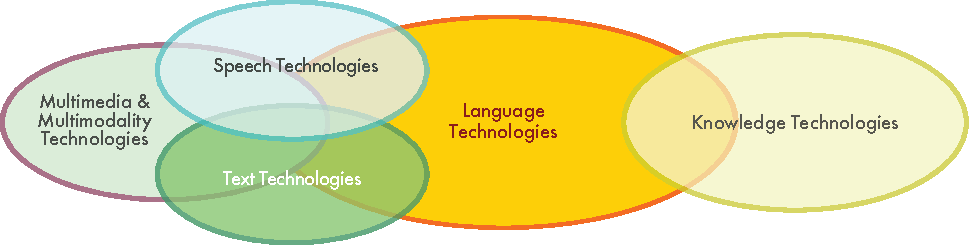
\includegraphics[width=\textwidth]{../_media/english/language_technologies}
  \caption{Language technology in context}
  \label{fig:ltincontext_en}
  \colorrule{grey3}{\textwidth}{1.5pt}
\end{figure*}

When we communicate, we combine language with other modes of communication and information media -- for example speaking can involve gestures and facial expressions. Digital texts link to pictures and sounds. Movies may contain language in spoken and written form. In other words, speech and text technologies overlap and interact with other multimodal communication and multimedia technologies.

In this section, we will discuss the main application areas of language technology, i.\,e., language checking, web search, speech interaction, and machine translation. These applications and basic technologies include 

\begin{itemize}
\item spelling correction,
\item authoring support,
\item computer-assisted language learning,
\item information retrieval,
\item information extraction,
\item text summarisation,
\item question answering,
\item speech recognition and
\item speech synthesis.
\end{itemize}

Language technology is an established area of research with an extensive set of introductory literature. The interested reader is referred to the following references:  \cite{jurafsky-martin01, manning-schuetze1, lt-world1, lt-survey1}.

Before discussing the above application areas, we will briefly describe the architecture of a typical LT system.

\subsection{Application Architectures}

Software applications for language processing typically consist of several components that mirror different aspects of language. While such applications are typically very complex, figure~\ref{fig:textprocessingarch_en} shows a highly simplified architecture of a typical text processing system. The first three modules handle the structure and meaning of the text input:

\begin{enumerate}
\item Pre-processing: cleans the data, analyses or removes formatting, detects the input language, handles the specific accented letters (\textit{á,é,í,ó,ö,ő,ú,ü,ű}) in Hungarian, and so on.
\item Grammatical analysis: finds the verb, its objects, modifiers and other parts of speech; detects the sentence structure.
\item Semantic analysis: performs disambiguation (i.\,e., computes the appropriate meaning of words in a given context); resolves anaphora (i.\,e., which pronouns refer to which nouns in the sentence); represents the meaning of the sentence in a machine-readable way.
\end{enumerate}

After analysing the text, task-specific modules can perform other operations, such as automatic summarisation and database look-ups.

In the remainder of this section, we firstly introduce the core application areas for language technology, and follow this with a brief overview of the state of LT research and education today, and a description of past and present research programmes. Finally, we present an expert estimate of core LT tools and resources for Hungarian in terms of various dimensions such as availability, maturity and quality. The general situation of LT for the Hungarian language is summarised in a matrix (figure~\ref{fig:lrlttable_en}) at the end of this chapter. LT support for Hungarian is also compared to other languages that are part of this series.

\begin{figure*}[htb]
  \colorrule{grey3}{\textwidth}{1.5pt}
  \center
  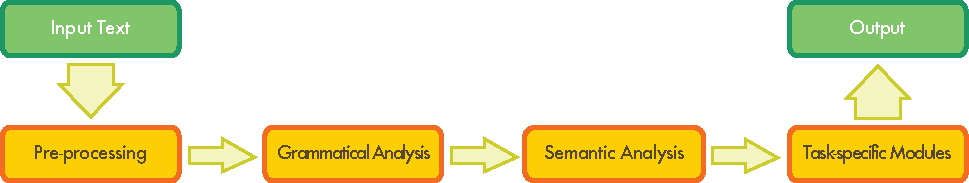
\includegraphics[width=\textwidth]{../_media/english/text_processing_app_architecture}
  \caption{A typical text processing architecture}
  \label{fig:textprocessingarch_en}
  \colorrule{grey3}{\textwidth}{1.5pt}
\end{figure*}

\subsection{Core Application Areas}

In this section, we focus on the most important LT tools and resources, and provide an overview of LT activities in Hungary. 

\subsubsection{Language Checking}

Anyone who has used a word processor such as Microsoft Word knows that it has a spell checker that highlights spelling mistakes and proposes corrections. The first spelling correction programs compared a list of extracted words against a dictionary of correctly spelled words. Today these programs are far more sophisticated. Using language-dependent algorithms for grammatical analysis, they detect errors related to morphology (e.\,g., plural formation) as well as syntax–related errors, such as a missing verb or a conflict of verb-subject agreement (e.\,g., \textit{she *write a letter}). However, most spell checkers will not find any errors in the following text \cite{zar1}:

\begin{quote}
  I have a spelling checker,\\
  It came with my PC.\\
  It plane lee marks four my revue\\
  Miss steaks aye can knot sea.
\end{quote}

Handling these kinds of errors usually requires an analysis of the context. For example: there are inflected word forms in Hungarian that can hold several meanings, e.g.: the word \textit{várunk} can be an inflected form of the verb \textit{vár}, or the noun \textit{vár} with possessive inflection. 

This type of analysis either needs to draw on language-specific grammars laboriously coded into the software by experts, or on a statistical language model. In this case, a model calculates the probability of a particular word as it occurs in a specific position (e.g., between the words that precede and follow it). For example: \textit{várunk} is probably not a verb if the sentence contains an other finite verb. A statistical language model can be automatically created by using a large amount of (correct) language data (called a text corpus). Most of these two approaches have been developed around data from English. Neither approach can transfer easily to Hungarian because it has a flexible word order and a richer inflection system.

\begin{figure*}[htb]
  \colorrule{grey3}{\textwidth}{1.5pt}
  \center
  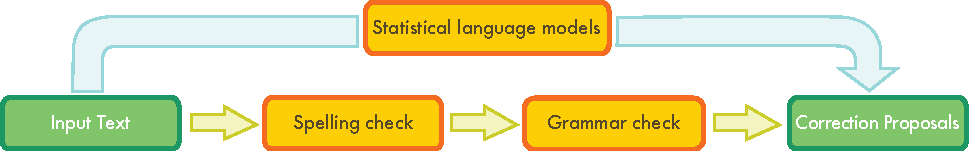
\includegraphics[width=\textwidth]{../_media/english/language_checking}
  \caption{Language checking (statistical; rule-based)}
  \label{fig:langcheckingaarch_en}
  \colorrule{grey3}{\textwidth}{1.5pt}
\end{figure*}

Language checking is not limited to word processors; it is also used in authoring support systems, i.e., software environments in which manuals and other documentation are written to special standards for complex IT, healthcare, engineering and other products. Fearing customer complaints about incorrect use and damage claims resulting from poorly understood instructions, companies are increasingly focusing on the quality of technical documentation while targeting the international market (via translation or localization) at the same time. Advances in natural language processing have led to the development of authoring support software, which helps the writer of technical documentation use vocabulary and sentence structures that are consistent with industry rules and (corporate) terminology restrictions.

\boxtext{The use of language checking is not limited to word processors. It also applies to authoring support systems.}

As Hungarian is a highly agglutinative language, a Hungarian spell checker must contain a morphological analyzer that handles the great number of affixes and complex words. The first spell checker for Hungarian has been developed by combining a spell checking system and a morphological model by a Hungarian SME called MorphoLogic \cite{morpho}, in the late 80s. Their program (\textit{Helyes-e?}) is available for MS Office, QuarkXPress, Adobe InDesign and other desktop publisher packages. MorphoLogic developed grammar and style checkers that recognise spelling errors based on the context. The program indicates possible mistakes and leaves it to the user to decide whether it is a real mistake.

An open source spell checker for Hungarian exists as well. Hunspell \cite{hunspell} is based on MySpell, and it has been integrated into OpenOffice, Mozilla Firefox 3, Mozilla Thunderbird and Google Chrome.

Besides spell checkers and authoring support, language checking is also important in the field of computer-assisted language learning. And language checking applications also automatically correct search engine queries, as found in Google's \textit{Did you mean\dots} suggestions.

\subsubsection{Web Search}

\begin{figure*}[htb]
  \colorrule{grey3}{\textwidth}{1.5pt}
  \center
  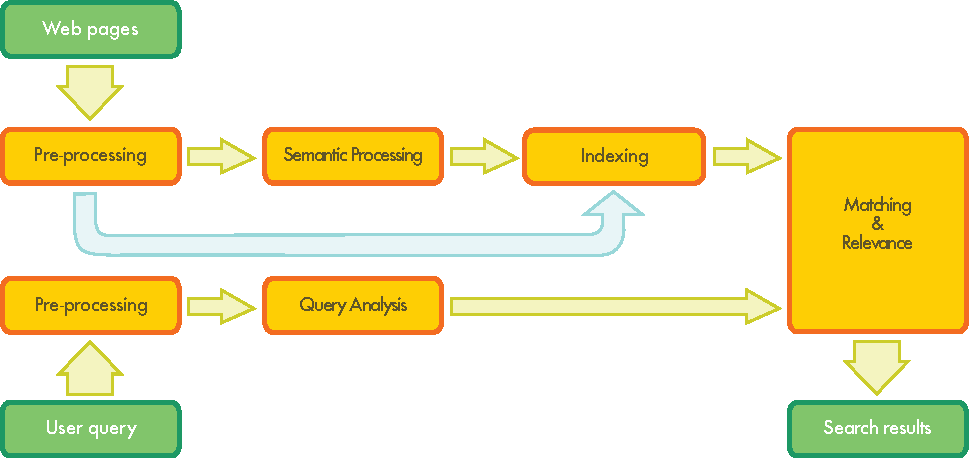
\includegraphics[width=\textwidth]{../_media/english/web_search_architecture}
  \caption{Web search}
  \label{fig:websearcharch_en}
  \colorrule{grey3}{\textwidth}{1.5pt}
 \end{figure*}

Searching the Web, intranets or digital libraries is probably the most widely used yet largely underdeveloped language technology application today. The Google search engine, which started in 1998, now handles about 80\% of all search queries \cite{spi1}. The verb \textit{guglizni} is commonly used in Hungarian, even though it has not made its way into printed dictionaries yet. The Google search interface and results page display has not significantly changed since the first version. Yet in the current version, Google offers spelling correction for misspelled words and has now incorporated basic semantic search capabilities that can improve search accuracy by analysing the meaning of terms in a search query context \cite{pc1}. The Google success story shows that a large volume of available data and efficient indexing techniques can deliver satisfactory results for a statistically-based approach.  

For more sophisticated information requests, it is essential to integrate deeper linguistic knowledge for text interpretation. Experiments using lexical resources such as machine-readable thesauri or ontological language resources (e.g., WordNet for English or Hungarian WordNet for Hungarian) have demonstrated improvements in finding pages using synonyms of the original search terms, such as \textit{atomenergia} [atomic energy], \textit{magenergia} [atomic power] and \textit{nukleáris energia} [nuclear energy], or even more loosely related terms.

\boxtext{The next generation of search engines will have to include much more sophisticated language technology.}

The next generation of search engines will have to include much more sophisticated language technology, in particular in order to deal with search queries consisting of a question or other sentence type rather than a list of keywords. For the query, ``Give me a list of all companies that were taken over by other companies in the last five years'', the LT system needs to analyse the sentence syntactically and semantically as well as provide an index to quickly retrieve relevant documents. A satisfactory answer will require syntactic parsing to analyse the grammatical structure of the sentence and determine that the user wants companies that have been acquired, not companies that acquired other companies. For the expression \textit{last five years}, the system needs to determine the relevant years. And, the query needs to be matched against a huge amount of unstructured data to find the piece or pieces of relevant information the user wants. This is called ``information retrieval'', and involves searching and ranking relevant documents. To generate a list of companies, the system also needs to recognise a particular string of words in a document as a company name, a process called ``named entity recognition''.

A more demanding challenge is matching a query in one language with documents in another language. Cross-lingual information retrieval involves automatically translating the query into all possible source languages and then translating the results back into the target language. 

Now that data is increasingly found in non-textual formats, there is a need for services that deliver multimedia information retrieval by searching images, audio files and video data. In the case of audio and video files, a speech recognition module must convert the speech content into text (or into a phonetic representation) that can then be matched against a user query.

For inflectional languages like Hungarian, it is important to be able to search for all the inflected forms of a word simultaneously, instead of having to enter each different form separately. For this purpose, several morphological parsers exist for Hungarian. NP chunkers for identifying noun phrases provide higher level parsing: a statistical and a rule-based application have been developed for Hungarian. 

Due to the variable word order characteristic of Hungarian, we cannot rely on exploiting particular linear configurations alone when syntactic parsers are developed. On the other hand, Hungarian is an agglutinative language with rich case marking, and morphological case markers and postpositions lend themselves to being used as cues for parsing. A database of Hungarian verbs and case markers of their arguments was developed at the Research Institute for Linguistics, which has been built in higher level parsing applications, e.g. for automatic acquisition of verb argument frames, or rule-based syntactic parsing. More syntactic parsers for Hungarian exist -- one of them was built in the Hungarian treebank (Szeged Treebank) and in a rule-based Hungarian-English machine translation program (MetaMorpho).

Focus on development for HLT companies and research institutes lies on providing trend- and text-analysis tools which integrate natural language processing tools to find the relevant information in unstructured text. For this purpose part-of-speech taggers, dependency parsers and named entity recognisers have been developed for Hungarian, which are mostly based on statistical learning algorithms.

A meta-search and clustering engine is PolyMeta \cite{polymeta}. It enables organisations and individuals to simultaneously search diverse information resources on the web with a common interface. It employs natural language processing and Information Retrieval algorithms in its query analysis and refinement, search strategy, relevancy ranking, focused drill-down and exploration of multi-dimensional information spaces.

Certainly, not only SMEs try to extract information by natural language processing tools. Several projects have been running in the academia with the aim of developing a model-based semantic search system, creating the framework of a unified Hungarian ontology, or creating a semantically structured, general purpose Hungarian concept set on the basis of the results and formalism of EuroWordNet language ontology (Hungarian WordNet).

\subsubsection{Speech Interaction}

Speech interaction is one of many application areas that depend on speech technology, i.\,e., technologies for processing spoken language. Speech interaction technology is used to create interfaces that enable users to interact in spoken language instead of using a graphical display, keyboard and mouse. Today, these voice user interfaces (VUI) are used for partially or fully automated telephone services provided by companies to customers, employees or partners. Business domains that rely heavily on VUIs include banking, supply chain, public transportation, and telecommunications. Other uses of speech interaction technology include interfaces to car navigation systems and the use of spoken language as an alternative to the graphical or touchscreen interfaces in smartphones.

\begin{figure*}[htb]
  \colorrule{grey3}{\textwidth}{1.5pt}
  \center
  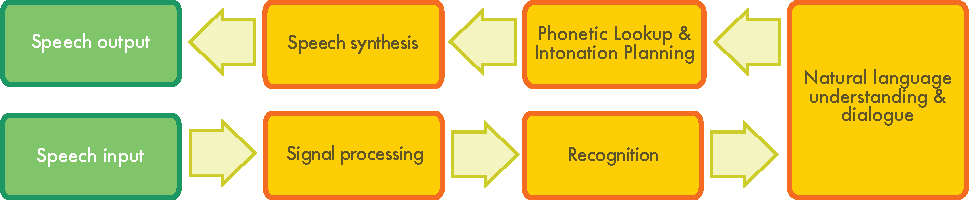
\includegraphics[width=\textwidth]{../_media/english/simple_speech-based_dialogue_architecture}
  \caption{Speech-based dialogue system}
  \label{fig:dialoguearch_en}
  \colorrule{grey3}{\textwidth}{1.5pt}
\end{figure*}

Speech interaction technology comprises four technologies: 

\begin{enumerate}
      \item Automatic speech recognition (ASR) determines which words are actually spoken in a given sequence of sounds uttered by a user.
      \item Natural language understanding analyses the syntactic structure of a user's utterance and interprets it according to the system in question.
      \item Dialogue management determines which action to take given the user input and system functionality.    
      \item Speech synthesis (text-to-speech or TTS) transforms the system's reply into sounds for the user.
    \end{enumerate}

One of the major challenges of ASR systems is to accurately recognise the words a user utters. This means restricting the range of possible user utterances to a limited set of keywords, or manually creating language models that cover a large range of natural language utterances. Using machine learning techniques, language models can also be generated automatically from speech corpora, i.e., large collections of speech audio files and text transcriptions. Restricting utterances usually forces people to use the voice user interface in a rigid way and can damage user acceptance; but the creation, tuning and maintenance of rich language models will significantly increase costs. VUIs that employ language models and initially allow a user to express their intent more flexibly -- prompted by a \textit{How may I help you?} greeting -- tend to be automated and are better accepted by users.

\boxtext{Speech interaction is the basis for creating interfaces that allow a user to interact with spoken language instead of a graphical display, keyboard and mouse.}

Companies tend to use pre-recorded utterances by professional speakers for generating the output of the voice user interface. For static utterances where the wording does not depend on particular contexts of use or personal user data, this can deliver a rich user experience. But more dynamic content in an utterance may suffer from unnatural intonation because bits of audio files have simply been strung together. Today's TTS systems are getting better (though they can still be optimised) at producing natural-sounding dynamic utterances. 

Interfaces in speech interaction have been considerably standardised during the last decade in terms of their various technological components. There has also been strong market consolidation in speech recognition and speech synthesis. The national markets in the G20 countries (economically resilient countries with high populations) have been dominated by just five global players, with Nuance (USA) and Loquendo (Italy) being the most prominent players in Europe. In 2011, Nuance announced the acquisition of Loquendo, which represents a further step in market consolidation.

Due to the specific characteristics of Hungarian, the widely used methods in Speech Interaction technology are difficult or impossible to adapt for Hungarian. However, the methods developed for Hungarian can be applied for similar languages, e.g. Finnish, Turkish, Arabic, in the field of TTS and ASR. 

The Hungarian TTS market is dominated by research groups at Budapest University of Technology and Economics \cite{bme}. The most widely used TTS system is Profivox, available since 2002, which has been built into SMS- and email-reader softwares, into in-car and mobilephone GPS systems, and into e-book- and screen-reader applications which can help the integration of blind people into information society. A high level interactive development tool is also available for supporting special research (psychology and prosody research). The software supports a supervised generation of speech stimuli with predefined acoustic and prosodic content, based on TTS technology. Hungarian pronunciation electronic dictionary also exists for 1.5 million word forms. This may be the basis of the development of a Hungarian TTS symbol conversion tool.

On the Hungarian ASR market there are additional smaller companies, such as Applied Logic Laboratory, Aitia, Digital Natives, as well as academic research groups, e.g. at the University of Szeged. In spite of the linguistic difficulties mentioned above, several speech recogniser applications for Hungarian have been developed over the last few years. One of them is a prosodic recogniser that was prepared by a cross-lingual study for agglutinative, fixed stressed languages, such as Hungarian and Finnish, about the segmentation of continuous speech on word level by examination of supra-segmental parameters. Another system helps the work of doctors: during examining the patient they dictate the diagnosis which will be automatically transcribed. Yet another one is a Hungarian computer assisted speech pronunciation learning and training system for speech handicapped and for language learning, which is adapted for some European languages, as well. Further application areas are call centres, dialogue systems, or indexing and searching media databases. 

Looking ahead, there will be significant changes, due to the spread of smartphones as a new platform for managing customer relationships, in addition to fixed telephones, the Internet and e-mail. This will also affect how speech interaction technology is used. In the long term, there will be fewer telephone-based VUIs, and spoken language apps will play a far more central role as a user-friendly input for smartphones. This will be largely driven by stepwise improvements in the accuracy of speaker-independent speech recognition via the speech dictation services already offered as centralised services to smartphone users.

\subsubsection{Machine Translation}

\begin{figure*}[htb]
  \colorrule{grey3}{\textwidth}{1.5pt}
  \center
  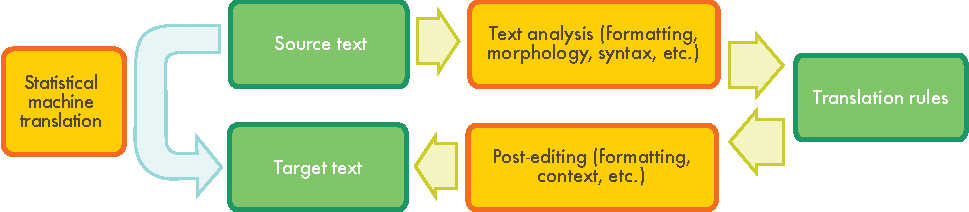
\includegraphics[width=\textwidth]{../_media/english/machine_translation}
  \caption{Machine translation (statistical; rule-based)}
  \label{fig:mtarch_en}
  \colorrule{grey3}{\textwidth}{1.5pt}
\end{figure*}

The idea of using digital computers to translate natural languages can be traced back to 1946 and was followed by substantial funding for research during the 1950s and again in the 1980s. 
Yet machine translation (MT) still cannot deliver on its initial promise of providing across-the-board automated translation.  

\boxtext{At its basic level, machine translation simply substitutes words in one natural language with words in another language.}

The most basic approach to machine translation is the automatic replacement of the words in a text written in one natural language with the equivalent words of another language. This can be useful in subject domains that have a very restricted, formulaic language such as weather reports. However, in order to produce a good translation of less restricted texts, larger text units (phrases, sentences, or even whole passages) need to be matched to their closest counterparts in the target language. The major difficulty is that human language is ambiguous. Ambiguity creates challenges on multiple levels, such as word sense disambiguation on the lexical level (a \textit{jaguar} is a brand of car or an animal) or the assignment of case on the syntactic level, for example:

\begin{itemize}
\item A rendőr látta az embert a távcsővel. 
\item A rendőr látta az embert a revolverrel.
\end{itemize}

One way to build an MT system is to use linguistic rules. For translations between closely related languages, a translation using direct substitution may be feasible in cases such as the above example. However, rule-based (or linguistic knowledge-driven) systems often analyse the input text and create an intermediary symbolic representation from which the target language text can be generated. The success of these methods is highly dependent on the availability of extensive lexicons with morphological, syntactic, and semantic information, and large sets of grammar rules carefully designed by skilled linguists. This is a very long and therefore costly process.

In the late 1980s when computational power increased and became cheaper, interest in statistical models for machine translation began to grow. Statistical models are derived from analysing bilingual text corpora, parallel corpora, such as the Europarl parallel corpus, which contains the proceedings of the European Parliament in 11 European languages. Given enough data, statistical MT works well enough to derive an approximate meaning of a foreign language text by processing parallel versions and finding plausible patterns of words. Unlike knowledge-driven systems, however, statistical (or data-driven) MT systems often generate ungrammatical output. Data-driven MT is advantageous because less human effort is required, and it can also cover special particularities of the language (e.\,g., idiomatic expressions) that are often ignored in knowledge-driven systems. 

The strengths and weaknesses of knowledge-driven and data-driven machine translation tend to be complementary, so that nowadays researchers focus on hybrid approaches that combine both methodologies. One such approach uses both knowledge-driven and data-driven systems, together with a selection module that decides on the best output for each sentence. However, results for sentences longer than, say, 12 words, will often be far from perfect. A more effective solution is to combine the best parts of each sentence from multiple outputs; this can be fairly complex, as corresponding parts of multiple alternatives are not always obvious and need to be aligned. 

\boxtext{Machine Translation is particularly challenging for the Hungarian language.}

Machine translation is particularly challenging for the Hungarian language. The free word order and split verb constructions pose problems for analysis; and extensive inflection is a challenge for generating words with proper case markings.

There are knowledge- and data-driven solutions on the Hungarian MT market, as well. MorphoLogic, a private R\&D company offers both desktop machine translation programs and online services. MorphoWord translates between English and Hungarian. Their MT system integrates rule-based and statistical methods, its main component being a parser that creates an intermediary representation, from which it produces the text in the target language.

Availability of large amounts of bilingual texts is actually the key in statistical MT. The Hunglish Corpus is a free sentence-aligned Hungarian-English parallel corpus of about 54.2 million words in 2.07 million sentences. At present this is the largest Hungarian-English parallel corpus. Sentence alignment was performed with hunalign, which is one of the most widely used sentence level aligners, developed by Hungarian researchers at Budapest University of Technology and Economics. The corpus may be searched through an online sentence search service \cite{hunglish}, which can be used as a raw translator or a smart bilingual lexicon.

The iTranslate4.eu \cite{it4eu} project started off in March 2010, which intends to provide online translation solution for all European languages. It does not only offer full coverage of EU languages, but also provides for each language pair the best quality available at the time, and mediates easy transfer to professional translators. The project is carried out by a consortium of European MT companies that have developed the best translation system for at least one language pair. The project has two Hungarian participants: the consortium leader is the Research Institute for Linguistics of Hungarian Academy of Sciences, and MorphoLogic provides the common API for the services.

The use of machine translation can significantly increase productivity provided the system is intelligently adapted to user-specific terminology and integrated into a workflow. Special systems for interactive translation support were developed, for example, at Kilgray \cite{memoq}. They provide translation tools, web-based terminology management systems and translation memories.

There is still a huge potential for improving the quality of MT systems. The challenges involve adapting language resources to a given subject domain or user area, and integrating the technology into workflows that already have term bases and translation memories. Another problem is that most of the current systems are English-centred and only support English from and into Hungarian. This leads to friction in the translation workflow and forces MT users to learn different lexicon coding tools for different systems.

Evaluation campaigns help to compare the quality of MT systems, the different approaches and the status of the systems for different language pairs. Figure~\ref{fig:euromatrix_hu} (p.~\pageref{fig:euromatrix_hu}), which was prepared during the EC Euromatrix+ project, shows the pair-wise performances obtained for 22 of the 23 official EU languages (Irish was not compared). The results are ranked according to a BLEU score, which indicates higher scores for better translations \cite{bleu1}. A human translator would normally achieve a score of around 80 points.

The best results (in green and blue) were achieved by languages that benefit from a considerable research effort in coordinated programmes and the existence of many parallel corpora (e.\,g., English, French, Dutch, Spanish and German). The languages with poorer results are shown in red. These languages either lack such development efforts or are structurally very different from other languages (e.\,g., Hungarian, Maltese and Finnish).

\subsection{Other Application Areas}

Building language technology applications involves a range of subtasks that do not always surface at the level of interaction with the user, but they provide significant service functionalities “behind the scenes” of the system in question. They all form important research issues that have now evolved into individual sub-disciplines of computational linguistics.  Question answering, for example, is an active area of research for which annotated corpora have been built and scientific competitions have been initiated. The concept of question answering goes beyond keyword-based searches (in which the search engine responds by delivering a collection of potentially relevant documents) and enables users to ask a concrete question to which the system provides a single answer. For example:

\textit{Question: How old was Neil Armstrong when he stepped on the moon?}\\
\textit{Answer: 38.}

While question answering is obviously related to the core area of web search, it is nowadays an umbrella term for such research issues as which different types of questions exist, and how they should be handled; how a set of documents that potentially contain the answer can be analysed and compared (do they provide conflicting answers?); and how specific information (the answer) can be reliably extracted from a document without ignoring the context. 

\boxtext{Language technology applications often provide significant service functionalities "behind the scenes” of larger software systems.}

Question answering is in turn related to information extraction (IE), an area that was extremely popular and influential when computational linguistics took a statistical turn in the early 1990s. IE aims to identify specific pieces of information in specific classes of documents, such as the key players in company takeovers as reported in newspaper stories. Another common scenario that has been studied is reports on terrorist incidents. The task here consists of mapping appropriate parts of the text to a template that specifies the perpetrator, target, time, location and results of the incident. Domain-specific template-filling is the central characteristic of IE, which makes it another example of a “behind the scenes” technology that forms a well-demarcated research area, which in practice needs to be embedded into a suitable application environment. 

    Text summarisation and text generation are two borderline areas that can act either as standalone applications or play a supporting role. Summarisation attempts to give the essentials of a long text in a short form, and is one of the features available in Microsoft Word. It mostly uses a statistical approach to identify the “important” words in a text (i.\,e., words that occur very frequently in the text in question but less frequently in general language use) and determine which sentences contain the most of these “important” words. These sentences are then extracted and put together to create the summary. In this very common commercial scenario, summarisation is simply a form of sentence extraction, and the text is reduced to a subset of its sentences. An alternative approach, for which some research has been carried out, is to generate brand new sentences that do not exist in the source text. 

\boxtext{For the Hungarian language, research in most text technologies is much less developed than for the English language.}

This requires a deeper understanding of the text, which means that so far this approach is far less robust. On the whole, a text generator is rarely used as a stand-alone application but is embedded into a larger software environment, such as a clinical information system that collects, stores and processes patient data. Creating reports is just one of many applications for text summarisation. 

For the Hungarian language, research in these text technologies is much less developed than for the English language. Question answering, information extraction, and summarization have been the focus of numerous open competitions in the USA since the 1990s, primarily organised by the government-sponsored organisations DARPA and NIST. These competitions have significantly improved the start-of-the-art, but their focus has mostly been on the English language. As a result, there are hardly any annotated corpora or other special resources needed to perform these tasks in Hungarian. When summarization systems use purely statistical methods, they are largely language-independent and a number of research prototypes are available. For text generation, reusable components have traditionally been limited to surface realization modules (generation grammars) and most of the available software is for the English language. There are, however, several named entity recognizer, biomedical information extracting, trend analysing and opinion mining systems for the Hungarian language.

\subsection{Educational Programmes}

Language technology is a very interdisciplinary field that involves the combined expertise of linguists, computer scientists, mathematicians, philosophers, psycholinguists, and neuroscientists among others. As a result, it has not acquired a clear, independent existence in the Hungarian faculty system yet, so in Hungary there is no university with an established department of Computational Linguistics. However, there are relevant programmes offered by related departments, such as the faculty of computer science or the faculty of linguistics. Some universities offer Master or Bachelor courses only, or modules in Language Technology to students of other courses of study. Many of these programs and courses have only been introduced recently. Currently, six Hungarian universities offer at least courses in the field of Language Technology.

In spite of the efforts in recent years to find the way of regular teaching of CL into the Hungarian faculty system, the education of next generation computational linguists does not achieve the required level. The aim of the Hungarian CL community is to develop a high quality curriculum of BSc-MSc-PhD sequence, which fits into the European standards. The relatively low salaries and scholarships of young researchers pose further problems, which could partly be solved by strengthening the relationships between research and industry.

\subsection{National Projects and Initiatives}

Similar to other countries, the beginnings of natural language processing in Hungary are connected with Machine Translation. The first attempts were made in the 1960s -- in those years from Russian to Hungarian. In the 1970s-1980s the lexicographers' work gave the impetus that led to the development of the first computational morphosyntactic systems for Hungarian. In those years there were no regular nationally financed projects, moreover, Hungary was separated from European support.

    After the political change, in the 1990s new sections were formed at universities (e.g. the Natural Language Processing Group at Szeged University) and in research institutes (e.g. the Department for Corpus Linguistics at the Research Institute for Linguistics). Since 2000, there has been a significant increase in the number of projects supported by European funds and nationally financed projects, supported mainly by the Fund of the Ministry of Education, or the Agency for Research Fund Management and Research Exploitation. 

    As a consequence, over the past decade a number of important electronic language resources (dictionaries, corpora, lexical databases) as well as processing resources (spell checking, morphological analyser etc.) have been developed. Activities however have not been synchronized, and not uncommonly similar resources have been developed in parallel at different locations (e.g. there are at least three morphological analysers for Hungarian). A range of different formalisms or standards have been used in these, which in the majority of cases are either incompatible or difficult to convert from; there is also a lack of documentation and in many cases copyright issues are unclear. Nevertheless, in recent years the international trends of standardisation and uniformisation of existing resources have reached Hungary as well. Several projects started off with the objective of integration and interoperability, e.g. creating a unified Hungarian ontology, or harmonising the different coding systems of separately developed morphological analysers.

    In 2008, prominent Hungarian academic institutions and R\&D companies formed the Hungarian Platform for Speech and Language Technology \cite{platform}, which aims to help sharing and integration of high quality knowledge accumulated in centres that worked in isolation beforehand; to work out detailed strategic and implementation plans and to help their subsequent implementation; to disseminate its analyses and proposals among the members of the IT sector; to represent the Hungarian interests at the international level; and to disseminate the achievements of the Platform among the potential users of the technology. Hungarian institutions have also been involved in the CLARIN project. 

    Along with many smaller scale projects that have now been completed, the above projects have led to the development of wide-ranging competence in the field of language technology as well as the creation of a basic technological infrastructure for Hungarian language tools and resources. Public funding for LT projects in Hungary and in Europe is still relatively low, however, when compared to the amount of money the USA spends on language translation and multilingual information access \cite{laz1}.  

As we have seen, previous programmes have led to the development of a number of LT tools and resources for the Hungarian language. The following section summarises the current state of LT support for Hungarian.
  
\subsection{Availability of Tools and Resources}

Figure~\ref{fig:lrlttable_en} provides a rating for language technology support for the Hungarian language. This rating of existing tools and resources was generated by leading experts in the field who provided estimates based on a scale from 0 (very low) to 6 (very high) using seven criteria.

\begin{figure*}[htb]
\centering
%\begin{tabular}{>{\columncolor{orange1}}p{.33\linewidth}ccccccc} % ORIGINAL
\begin{tabular}{>{\columncolor{orange1}}p{.33\linewidth}@{\hspace*{6mm}}c@{\hspace*{6mm}}c@{\hspace*{6mm}}c@{\hspace*{6mm}}c@{\hspace*{6mm}}c@{\hspace*{6mm}}c@{\hspace*{6mm}}c}
\rowcolor{orange1}
 \cellcolor{white}&\begin{sideways}\makecell[l]{Quantity}\end{sideways}
&\begin{sideways}\makecell[l]{\makecell[l]{Availability} }\end{sideways} &\begin{sideways}\makecell[l]{Quality}\end{sideways}
&\begin{sideways}\makecell[l]{Coverage}\end{sideways} &\begin{sideways}\makecell[l]{Maturity}\end{sideways} &\begin{sideways}\makecell[l]{Sustainability}\end{sideways} &\begin{sideways}\makecell[l]{Adaptability}\end{sideways} \\ \addlinespace
\multicolumn{8}{>{\columncolor{orange2}}l}{Language Technology: Tools, Technologies and Applications} \\ \addlinespace
Speech Recognition	&3&0&4&2&4&3&3 \\ \addlinespace
Speech Synthesis &4&3&4&4&5&3&3\\ \addlinespace
Grammatical analysis &4.5&2&4&4.5&4&3&4.5\\ \addlinespace
Semantic analysis &0.6&2&2.5&0.5&0&0&2\\ \addlinespace
Text generation &0&0&0&0&0&0&0\\ \addlinespace
Machine translation &6&1&4&3&6&5&6\\ \addlinespace
\multicolumn{8}{>{\columncolor{orange2}}l}{Language Resources: Resources, Data and Knowledge Bases} \\ \addlinespace
Text corpora &3.5&6&5.5&5.5&6&6&4\\ \addlinespace
Speech corpora &2&2&4&2&4&4&0\\ \addlinespace
Parallel corpora &6&4&4.5&2.5&6&6&6\\ \addlinespace
Lexical resources &3&1&3.5&3.5&3.5&3.5&4.5\\ \addlinespace
Grammars &3&3&5&5&6&4&3\\
\end{tabular}
\caption{State of language technology support for Hungarian}
\label{fig:lrlttable_en}
\end{figure*}

The key results for Hungarian language technology can be summed up as follows:

\begin{itemize}
      \item While several specific corpora of high quality exist, a very large syntactically annotated corpus is not available. However, there is a syntactically highly elaborately annotated corpus for Hungarian (1.2 million tokens). The corpus is available for free, which results in a wide range applications developed based on the corpus.
      \item Many of the resources lack standardization, i.e., even if they exist, they are not addressing sustainability; concerted programs and initiatives are needed to standardize data and interchange formats.
      \item The standard preprocessing steps (tokenization, morphology, shallow parsing, etc.) are completed for Hungarian, but treating the more difficult semantics requires further research. 
      \item The more linguistic and semantic knowledge a tool draws on, the more gaps there are in the technology (text analysis versus text interpretation). There is a need for far more effort to support deep linguistic processing.
      \item Research has been successful in designing particularly high quality software, but many of the resources are not standardised and cannot be sustained effectively. A concerted program is required to standardise data and interchange formats.
      \item There is a lack of annotated corpora with syntactic, semantic and discourse structure mark-up. Again, the situation gets worse as the need for more deep linguistic and semantic information grows.
      \item Standards do exist for semantics in the sense of world knowledge (RDF, OWL, etc.); they are, however, not easily applicable to NLP tasks.
      \item Speech Recognition and Machine Translation of Hungarian is studied at several universities and workplaces, but free tools and data are currently not available. It is a typical phenomenon at the Hungarian NLP market that the number of free databases and open source programs is quite low.
    \end{itemize}

To conclude, in a number of specific areas of Hungarian language research, we have softwares with limited functionality available today. Obviously, further research efforts are required to meet the current deficit in processing texts on a deeper semantic level and to address the lack of resources such as speech corpora for speech recognition.

\subsection{Cross-language comparison}

\begin{figure*}[tb]
  \small
  \centering
  \begin{tabular}
  { % defines color for each column.
  >{\columncolor{corange5}}p{.13\linewidth}@{\hspace{.040\linewidth}}
  >{\columncolor{corange4}}p{.13\linewidth}@{\hspace{.040\linewidth}}
  >{\columncolor{corange3}}p{.13\linewidth}@{\hspace{.040\linewidth}}
  >{\columncolor{corange2}}p{.13\linewidth}@{\hspace{.040\linewidth}}
  >{\columncolor{corange1}}p{.13\linewidth} 
  }
  \multicolumn{1}{>{\columncolor{white}}c@{\hspace{.040\linewidth}}}{\textbf{Excellent}} & 
  \multicolumn{1}{@{}>{\columncolor{white}}c@{\hspace{.040\linewidth}}}{\textbf{Good}} &
  \multicolumn{1}{@{}>{\columncolor{white}}c@{\hspace{.040\linewidth}}}{\textbf{Moderate}} &
  \multicolumn{1}{@{}>{\columncolor{white}}c@{\hspace{.040\linewidth}}}{\textbf{Fragmentary}} &
  \multicolumn{1}{@{}>{\columncolor{white}}c}{\textbf{Weak/no}} \\ 
  \multicolumn{1}{>{\columncolor{white}}c@{\hspace{.040\linewidth}}}{\textbf{support}} & 
  \multicolumn{1}{@{}>{\columncolor{white}}c@{\hspace{.040\linewidth}}}{\textbf{support}} &
  \multicolumn{1}{@{}>{\columncolor{white}}c@{\hspace{.040\linewidth}}}{\textbf{support}} &
  \multicolumn{1}{@{}>{\columncolor{white}}c@{\hspace{.040\linewidth}}}{\textbf{support}} &
  \multicolumn{1}{@{}>{\columncolor{white}}c}{\textbf{support}} \\ \addlinespace
  
& \vspace*{0.5mm}English
& \vspace*{0.5mm}
Czech \newline 
Dutch \newline 
Finnish \newline 
French \newline 
German \newline   
Italian \newline  
Portuguese \newline 
Spanish \newline
& \vspace*{0.5mm}Basque \newline 
Bulgarian \newline 
Catalan \newline 
Danish \newline 
Estonian \newline 
Galician\newline 
Greek \newline  
Hungarian  \newline
Irish \newline  
Norwegian \newline 
Polish \newline 
Serbian \newline 
Slovak \newline 
Slovene \newline 
Swedish \newline
& \vspace*{0.5mm}
Croatian \newline 
Icelandic \newline  
Latvian \newline 
Lithuanian \newline 
Maltese \newline 
Romanian\\
\end{tabular}
\caption{Speech processing: state of language technology support for 30 European languages}
\label{fig:speech_cluster_en}
\end{figure*}

\begin{figure*}[tb]
  \small
  \centering
  \begin{tabular}
  { % defines color for each column.
  >{\columncolor{corange5}}p{.13\linewidth}@{\hspace{.040\linewidth}}
  >{\columncolor{corange4}}p{.13\linewidth}@{\hspace{.040\linewidth}}
  >{\columncolor{corange3}}p{.13\linewidth}@{\hspace{.040\linewidth}}
  >{\columncolor{corange2}}p{.13\linewidth}@{\hspace{.040\linewidth}}
  >{\columncolor{corange1}}p{.13\linewidth} 
  }
  \multicolumn{1}{>{\columncolor{white}}c@{\hspace{.040\linewidth}}}{\textbf{Excellent}} & 
  \multicolumn{1}{@{}>{\columncolor{white}}c@{\hspace{.040\linewidth}}}{\textbf{Good}} &
  \multicolumn{1}{@{}>{\columncolor{white}}c@{\hspace{.040\linewidth}}}{\textbf{Moderate}} &
  \multicolumn{1}{@{}>{\columncolor{white}}c@{\hspace{.040\linewidth}}}{\textbf{Fragmentary}} &
  \multicolumn{1}{@{}>{\columncolor{white}}c}{\textbf{Weak/no}} \\ 
  \multicolumn{1}{>{\columncolor{white}}c@{\hspace{.040\linewidth}}}{\textbf{support}} & 
  \multicolumn{1}{@{}>{\columncolor{white}}c@{\hspace{.040\linewidth}}}{\textbf{support}} &
  \multicolumn{1}{@{}>{\columncolor{white}}c@{\hspace{.040\linewidth}}}{\textbf{support}} &
  \multicolumn{1}{@{}>{\columncolor{white}}c@{\hspace{.040\linewidth}}}{\textbf{support}} &
  \multicolumn{1}{@{}>{\columncolor{white}}c}{\textbf{support}} \\ \addlinespace
  
& \vspace*{0.5mm} English 
& \vspace*{0.5mm} 
French \newline 
Spanish
& \vspace*{0.5mm}
Catalan \newline 
Dutch \newline 
German \newline 
Hungarian \newline
Italian \newline 
Polish \newline 
Romanian \newline 
& \vspace*{0.5mm}Basque \newline 
Bulgarian \newline 
Croatian \newline 
Czech \newline
Danish \newline 
Estonian \newline 
Finnish \newline 
Galician \newline 
Greek \newline 
Icelandic \newline 
Irish \newline 
Latvian \newline 
Lithuanian \newline 
Maltese \newline 
Norwegian \newline 
Portuguese \newline 
Serbian \newline 
Slovak \newline 
Slovene \newline 
Swedish \newline 
\end{tabular}
\caption{Machine translation: state of language technology support for 30 European languages}
\label{fig:mt_cluster_en}
\end{figure*}

\begin{figure*}[tb]
  \small
  \centering
  \begin{tabular}
  { % defines color for each column.
  >{\columncolor{corange5}}p{.13\linewidth}@{\hspace{.040\linewidth}}
  >{\columncolor{corange4}}p{.13\linewidth}@{\hspace{.040\linewidth}}
  >{\columncolor{corange3}}p{.13\linewidth}@{\hspace{.040\linewidth}}
  >{\columncolor{corange2}}p{.13\linewidth}@{\hspace{.040\linewidth}}
  >{\columncolor{corange1}}p{.13\linewidth} 
  }
  \multicolumn{1}{>{\columncolor{white}}c@{\hspace{.040\linewidth}}}{\textbf{Excellent}} & 
  \multicolumn{1}{@{}>{\columncolor{white}}c@{\hspace{.040\linewidth}}}{\textbf{Good}} &
  \multicolumn{1}{@{}>{\columncolor{white}}c@{\hspace{.040\linewidth}}}{\textbf{Moderate}} &
  \multicolumn{1}{@{}>{\columncolor{white}}c@{\hspace{.040\linewidth}}}{\textbf{Fragmentary}} &
  \multicolumn{1}{@{}>{\columncolor{white}}c}{\textbf{Weak/no}} \\ 
  \multicolumn{1}{>{\columncolor{white}}c@{\hspace{.040\linewidth}}}{\textbf{support}} & 
  \multicolumn{1}{@{}>{\columncolor{white}}c@{\hspace{.040\linewidth}}}{\textbf{support}} &
  \multicolumn{1}{@{}>{\columncolor{white}}c@{\hspace{.040\linewidth}}}{\textbf{support}} &
  \multicolumn{1}{@{}>{\columncolor{white}}c@{\hspace{.040\linewidth}}}{\textbf{support}} &
  \multicolumn{1}{@{}>{\columncolor{white}}c}{\textbf{support}} \\ \addlinespace

& \vspace*{0.5mm}English
& \vspace*{0.5mm}
  Dutch \newline 
  French \newline 
  German \newline 
  Italian \newline 
  Spanish
& \vspace*{0.5mm}Basque \newline 
  Bulgarian \newline 
  Catalan \newline 
  Czech \newline 
  Danish \newline 
  Finnish \newline 
  Galician \newline 
  Greek \newline 
  Hungarian \newline 
  Norwegian \newline 
  Polish \newline 
  Portuguese \newline 
  Romanian \newline 
  Slovak \newline 
  Slovene \newline 
  Swedish \newline 
& \vspace*{0.5mm}
  Croatian \newline 
  Estonian \newline 
  Icelandic \newline 
  Irish \newline 
  Latvian \newline 
  Lithuanian \newline 
  Maltese \newline 
  Serbian \\
  \end{tabular}
\caption{Text analysis: state of language technology support for 30 European languages}
\label{fig:text_cluster_en}
\end{figure*}

\begin{figure*}[tb]
  \small
  \centering
  \begin{tabular}
  { % defines color for each column.
  >{\columncolor{corange5}}p{.13\linewidth}@{\hspace{.040\linewidth}}
  >{\columncolor{corange4}}p{.13\linewidth}@{\hspace{.040\linewidth}}
  >{\columncolor{corange3}}p{.13\linewidth}@{\hspace{.040\linewidth}}
  >{\columncolor{corange2}}p{.13\linewidth}@{\hspace{.040\linewidth}}
  >{\columncolor{corange1}}p{.13\linewidth} 
  }
  \multicolumn{1}{>{\columncolor{white}}c@{\hspace{.040\linewidth}}}{\textbf{Excellent}} & 
  \multicolumn{1}{@{}>{\columncolor{white}}c@{\hspace{.040\linewidth}}}{\textbf{Good}} &
  \multicolumn{1}{@{}>{\columncolor{white}}c@{\hspace{.040\linewidth}}}{\textbf{Moderate}} &
  \multicolumn{1}{@{}>{\columncolor{white}}c@{\hspace{.040\linewidth}}}{\textbf{Fragmentary}} &
  \multicolumn{1}{@{}>{\columncolor{white}}c}{\textbf{Weak/no}} \\ 
  \multicolumn{1}{>{\columncolor{white}}c@{\hspace{.040\linewidth}}}{\textbf{support}} & 
  \multicolumn{1}{@{}>{\columncolor{white}}c@{\hspace{.040\linewidth}}}{\textbf{support}} &
  \multicolumn{1}{@{}>{\columncolor{white}}c@{\hspace{.040\linewidth}}}{\textbf{support}} &
  \multicolumn{1}{@{}>{\columncolor{white}}c@{\hspace{.040\linewidth}}}{\textbf{support}} &
  \multicolumn{1}{@{}>{\columncolor{white}}c}{\textbf{support}} \\ \addlinespace
    
& \vspace*{0.5mm}English
& \vspace*{0.5mm} 
    Czech \newline 
    Dutch \newline 
    French \newline 
    German \newline 
    Hungarian \newline
    Italian \newline
    Polish \newline
    Spanish \newline
    Swedish \newline 
& \vspace*{0.5mm} Basque\newline 
    Bulgarian\newline 
    Catalan \newline 
    Croatian \newline 
    Danish \newline 
    Estonian \newline 
    Finnish \newline 
    Galician \newline 
    Greek \newline 
    Norwegian \newline 
    Portuguese \newline 
    Romanian \newline 
    Serbian \newline 
    Slovak \newline 
    Slovene \newline
&  \vspace*{0.5mm}
    Icelandic \newline 
    Irish \newline 
    Latvian \newline 
    Lithuanian \newline 
    Maltese  \\
  \end{tabular}
  \caption{Speech and text resources: State of support for 30 European languages}  
  \label{fig:resources_cluster_en}
\end{figure*}

The current state of LT support varies considerably from one language community to another. In order to compare the situation between languages, this section will present an evaluation based on two sample application areas (machine translation and speech processing) and one underlying technology (text analysis), as well as basic resources needed for building LT applications. The languages were categorised using the following five-point scale: 

\begin{enumerate}
\item Excellent support
\item Good support
\item Moderate support
\item Fragmentary support
\item Weak or no support
\end{enumerate}

LT support was measured according to the following criteria:

\textbf{Speech Processing:} Quality of existing speech recognition technologies, quality of existing speech synthesis technologies, coverage of domains, number and size of existing speech corpora, amount and variety of available speech-based applications.

\textbf{Machine Translation:} Quality of existing MT technologies, number of language pairs covered, coverage of linguistic phenomena and domains, quality and size of existing parallel corpora, amount and variety of available MT applications.

\textbf{Text Analysis:} Quality and coverage of existing text analysis technologies (morphology, syntax, semantics), coverage of linguistic phenomena and domains, amount and variety of available applications, quality and size of existing (annotated) text corpora, quality and coverage of existing lexical resources (e.\,g., WordNet) and grammars.

\textbf{Resources:} Quality and size of existing text corpora, speech corpora and parallel corpora, quality and coverage of existing lexical resources and grammars.

Figures~\ref{fig:speech_cluster_en} to~\ref{fig:resources_cluster_en} show that, thanks to large-scale LT funding in recent decades, the Hungarian language is quite well equipped compared to other. But LT resources and tools for Hungarian clearly do not yet reach the quality and coverage of comparable resources and tools for the English language, which is in the lead in almost all LT areas. And there are still plenty of gaps in English language resources with regard to high quality applications.

For speech processing, current technologies perform well enough to be successfully integrated into a number of industrial applications such as spoken dialogue and dictation systems. Today's text analysis components and language resources already cover the linguistic phenomena of Hungarian to a certain extent and form part of many applications involving mostly shallow natural language processing, e.g. spelling correction and some information extraction tasks.

However, for building more sophisticated applications, such as machine translation, there is a clear need for resources and technologies that cover a wider range of linguistic aspects and allow a deep semantic analysis of the input text. By improving the quality and coverage of these basic resources and technologies, we shall be able to open up new opportunities for tackling a vast range of advanced application areas, including high-quality machine translation.

\subsection{Conclusions}

\emph{In this series of white papers, we have made an important effort by assessing the language technology support for 30 European languages, and by providing a high-level comparison across these languages. By identifying the gaps, needs and deficits, the European language technology community and its related stakeholders are now in a position to design a large scale research and development programme aimed at building a truly multilingual, technology-enabled communication across Europe.}

The results of this white paper series show that there is a dramatic difference in language technology support for the various European languages. While there are good quality software and resources available for some languages and application areas, others, usually smaller languages, have substantial gaps. Many languages lack basic technologies for text analysis and the essential resources. Others have basic tools and resources but the implementation of for example semantic methods is still far away. Therefore a large-scale effort is needed to attain the ambitious goal of providing high-quality language technology support for all European languages, for example through high quality machine translation. 

In the case of the Hungarian language, we can be cautiously optimistic about the current state of language technology support. There is a viable LT research community in Hungary, which has been supported in the past mostly by national funds. And a number of large-scale resources and state-of-the-art technologies have been produced and distributed for Hungarian. However, the scope of the resources and the range of tools are still very limited when compared to the resources and tools for the English language, and they are simply not sufficient in quality and quantity to develop the kind of technologies required to support a truly multilingual knowledge society.

Nor can we simply transfer technologies already developed and optimised for the English language to handle Hungarian. English-based systems for parsing (syntactic and grammatical analysis of sentence structure) typically perform far less well on Hungarian texts, due to the specific characteristics of the Hungarian language.

There is a relatively small language technology industry at work on the Hungarian language. Thus the Hungarian NLP market is dominated by research groups at universities and academic institutes, however there are additional smaller companies on the market.  

Our findings lead to the conclusion that the only way forward is to make a substantial effort to create language technology resources for Hungarian, as a means to drive forward research, innovation and development. The need for large amounts of data and the extreme complexity of language technology systems makes it vital to develop an infrastructure and a coherent research organisation to spur greater sharing and cooperation.

Finally there is a lack of continuity in research and development funding. Short-term coordinated programmes tend to alternate with periods of sparse or zero funding. In addition, there is an overall lack of coordination with programmes in other EU countries and at the European Commission level.

The long term goal of META-NET is to enable the creation of high-quality language technology for all languages. This requires all stakeholders -- in politics, research, business, and society -- to unite their efforts. The resulting technology will help tear down existing barriers and build bridges between Europe’s languages, paving the way for political and economic unity through cultural diversity. 
\end{multicols}

\clearpage

\ssection[About META-NET]{About META-NET}
\label{meta-net_en}

\begin{multicols}{2}
META-NET is a Network of Excellence funded by the European Commission. The network currently consists of 54 members from 33 European countries. META-NET fosters the Multilingual Europe Technology Alliance (META), a growing community of language technology professionals and organisations in Europe. META-NET cooperates with other initiatives like the Common Language Resources and Technology Infrastructure (CLARIN), which is helping establish digital humanities research in Europe. META-NET fosters the technological foundations for a truly multilingual European information society that:

\begin{itemize}
\item makes communication and cooperation possible across languages;
\item provides equal access to information and knowledge in any language;
\item offers advanced and affordable networked information technology to European citizens.
\end{itemize}

META-NET stimulates and promotes multilingual technologies for all European languages. The technologies enable automatic translation, content production, information processing and knowledge management for a wide variety of applications and subject domains. The network wants to improve current approaches, so better communication and cooperation across languages can take place. Europeans have an equal right to information and knowledge regardless of language.

META-NET launched on 1 February 2010 with the goal of advancing research in language technology (LT). The network supports a Europe that unites as a single digital market and information space. META-NET has conducted several activities that further its goals. META-VISION, META-SHARE and META-RESEARCH are the network’s three lines of action.

\textbf{META-VISION} fosters a dynamic and influential stakeholder community that unites around a shared vision and a common strategic research agenda (SRA). The main focus of this activity is to build a coherent and cohesive LT community in Europe by bringing together representatives from highly fragmented and diverse groups of stakeholders. In the first year of META-NET, presentations at the FLaReNet Forum (Spain), Language Technology Days (Luxembourg), JIAMCATT 2010 (Luxembourg), LREC 2010 (Malta), EAMT 2010 (France) and ICT 2010 (Belgium) centred on public outreach. According to initial estimates, META-NET has already contacted more than 2,500 LT professionals to develop its goals and visions with them. At the META-FORUM 2010 event in Brussels, META-NET communicated the initial results of its vision building process to more than 250 participants. In a series of interactive sessions, the participants provided feedback on the visions presented by the network. 

\textbf{META-SHARE} creates an open, distributed facility for exchanging and sharing resources. The peer-to-peer network of repositories will contain language data, tools and web services that are documented with high-quality metadata and organised in standardised categories. The resources can be readily accessed and uniformly searched. The available resources include free, open source materials as well as restricted, commercially available, fee-based items. META-SHARE targets existing language data, tools and systems as well as new and emerging products that are required for building and evaluating new technologies, products and services. The reuse, combination, repurposing and re-engineering of language data and tools plays a crucial role. META-SHARE will eventually become a critical part of the LT marketplace for developers, localisation experts, researchers, translators and language professionals from small, mid-sized and large enterprises. META-SHARE addresses the full development cycle of LT—from research to innovative products and services. A key aspect of this activity is establishing META-SHARE as an important and valuable part of a European and global infrastructure for the LT community. 

\textbf{META-RESEARCH} builds bridges to related technology fields. This activity seeks to leverage advances in other fields and to capitalise on innovative research that can benefit language technology. In particular, this activity wants to bring more semantics into machine translation (MT), optimise the division of labour in hybrid MT, exploit context when computing automatic translations and prepare an empirical base for MT. META-RESEARCH is working with other fields and disciplines, such as machine learning and the Semantic Web community. META-RESEARCH focuses on collecting data, preparing data sets and organising language resources for evaluation purposes; compiling inventories of tools and methods; and organising workshops and training events for members of the community. This activity has already clearly identified aspects of MT where semantics can impact current best practices. In addition, the activity has created recommendations on how to approach the problem of integrating semantic information in MT. META-RESEARCH is also finalising a new language resource for MT, the Annotated Hybrid Sample MT Corpus, which provides data for English-German, English-Spanish and English-Czech language pairs. META-RESEARCH has also developed software that collects multilingual corpora that are hidden on the Web.
\end{multicols}

\cleardoublepage

\appendix
\addtocontents{toc}{\protect\bigskip}

\bsection[Hivatkozások -- References]{Hivatkozások --- References}
\bibliographystyle{plain}
\bibliography{hungarian}
  
\cleardoublepage

\bsection[META-NET tagok -- META-NET Members]{META-NET tagok --- META-NET Members}
\label{metanetmembers}

\small
\begin{longtable}{llp{105mm}}
  Ausztria & \textcolor{grey1}{Austria} & Zentrum für Translationswissenschaft, Universität Wien: Gerhard Budin\\ \addlinespace
  Belgium & \textcolor{grey1}{Belgium} & Computational Linguistics and Psycholinguistics Research Centre, Univ. of Antwerp: Walter Daelemans\\ \addlinespace
  & & Centre for Proc. Speech and Images, Univ. of Leuven: Dirk van Compernolle \\ \addlinespace
  Bulgária & \textcolor{grey1}{Bulgaria} & Inst. for Bulgarian Lang., Bulgarian Academy of Sciences: Svetla Koeva \\ \addlinespace
  Ciprus & \textcolor{grey1}{Cyprus} & Lang. Centre, School of Humanities: Jack Burston \\ \addlinespace
  Csehország & \textcolor{grey1}{Czech Republic} & Inst. of Formal and Applied Linguistics, Charles Univ. in Prague: Jan Hajic \\ \addlinespace
  Dánia &  \textcolor{grey1}{Denmark} & Centre for Lang. Technology, Univ. of Copenhagen: Bolette Sandford Pedersen, Bente Maegaard\\ \addlinespace
  Egyesült Királyság & \textcolor{grey1}{UK} & Inst. for Lang., Cognition and Computation, Center for Speech Technology Research, Univ. of Edinburgh: Steve Renals \\ \addlinespace 
  & & Research Inst. of Informatics and Lang. Proc., Univ. of Wolverhampton: Ruslan Mitkov \\ \addlinespace 
  & & School of Computer Science, Univ. of Manchester: Sophia Ananiandou \\ \addlinespace 
  Észtország & \textcolor{grey1}{Estonia} & Inst. of Computer Science, Univ. of Tartu: Tiit Roosmaa\\ \addlinespace
  Finnország & \textcolor{grey1}{Finland} & Computational Cognitive Systems Research Group, Aalto Univ.: Timo Honkela\\ \addlinespace
  & & Dept. of General Linguistics, Univ. of Helsinki: Kimmo Koskenniemi, Krister Linden \\ \addlinespace
  Franciaország & \textcolor{grey1}{France} & Centre National de la Recherche Scientifique, Laboratoire d'Informatique pour la Mécanique et les Sciences de l'Ingénieur: Joseph Mariani \\ \addlinespace
  & & Evaluations and Lang. Resources Distribution Agency: Khalid Choukri\\ \addlinespace 
  Görögország & \textcolor{grey1}{Greece} & Inst. for Lang. and Speech Proc., R.C. “Athena”: Stelios Piperidis\\ \addlinespace
   Hollandia & \textcolor{grey1}{Netherlands} & Utrecht Inst. of Linguistics, Utrecht Univ.: Jan Odijk\\ \addlinespace 
  & & Computational Linguistics, Univ. of Groningen: Gertjan van Noord\\ \addlinespace
   Horvátország & \textcolor{grey1}{Croatia} & Inst. of Linguistics, Faculty of Humanities and Social Science, Univ. of Zagreb: Marko Tadić \\ \addlinespace
    Írország & \textcolor{grey1}{Ireland} & School of Computing, Dublin City Univ.: Josef van Genabith\\ \addlinespace
  Izland & \textcolor{grey1}{Iceland} & School of Humanities, Univ. of Iceland: Eirikur Rögnvaldsson\\ \addlinespace
  Lengyelország & \textcolor{grey1}{Poland} & Inst. of Computer Science, Polish Academy of Sciences: Adam Przepiórkowski, Maciej Ogrodniczuk \\ \addlinespace
  & & Univ. of Łódź: Barbara Lewandowska-Tomaszczyk, Piotr Pęzik\\ \addlinespace
  & & Dept. of Computer Linguistics and Artificial Intelligence, Adam Mickiewicz Univ.: Zygmunt Vetulani \\ \addlinespace
  Lettország & \textcolor{grey1}{Latvia} & Tilde: Andrejs Vasiljevs\\ \addlinespace 
  & & Inst. of Mathematics and Computer Science, Univ. of Latvia: Inguna Skadina\\ \addlinespace
  Litvánia & \textcolor{grey1}{Lithuania} & Inst. of the Lithuanian Lang.: Jolanta Zabarskaitė\\ \addlinespace
  Luxemburg & \textcolor{grey1}{Luxembourg} & Arax Ltd.: Vartkes Goetcherian\\ \addlinespace
  Magyarország & \textcolor{grey1}{Hungary} & Research Inst. for Linguistics, Hungarian Academy of Sciences: Tamás Váradi\\  \addlinespace
  & & Dept. of Telecommunications and Media Informatics, Budapest Univ. of Technology and Economics: Géza Németh and Gábor Olaszy\\ \addlinespace
  Málta & \textcolor{grey1}{Malta} & Dept. Intelligent Computer Systems, Univ. of Malta: Mike Rosner\\ \addlinespace
  Németország & \textcolor{grey1}{Germany} & DFKI (German Research Centre for Artificial Intelligence): Hans Uszkoreit, Georg Rehm\\ \addlinespace
  & & Human Lang. Technology and Pattern Recognition, RWTH Aachen Univ.: Hermann Ney \\ \addlinespace
  & & Dept. of Computational Linguistics, Saarland Univ.: Manfred Pinkal\\ \addlinespace
  Norvégia & \textcolor{grey1}{Norway} & Dept. of Linguistic, Univ. of Bergen: Koenraad De Smedt\\ \addlinespace 
  & & Dept. of Informatics, Lang. Technology Group, Univ. of Oslo: Stephan Oepen \\ \addlinespace
  Olaszország & \textcolor{grey1}{Italy} & Consiglio Nazionale Ricerche, Istituto di Linguistica Computazionale “Antonio Zampolli”: Nicoletta Calzolari\\ \addlinespace
  & & Human Lang. Technology, Fondazione Bruno Kessler: Bernardo Magnini\\ \addlinespace
  Portugália & \textcolor{grey1}{Portugal} & Dept. of Informatics, Univ. of Lisbon: Antonio Branco\\ \addlinespace
  & & Spoken Lang. Systems Lab., Inst. for Systems Engineering and Computers: Isabel Trancoso \\ \addlinespace
  Románia & \textcolor{grey1}{Romania} & Research Inst. for Artificial Intelligence, Romanian Academy of Sciences: Dan Tufis \\ \addlinespace
  & & Faculty of Computer Science, Univ. Alexandru Ioan Cuza: Dan Cristea \\ \addlinespace
  Spanyolország & \textcolor{grey1}{Spain} & Barcelona Media: Toni Badia \\ \addlinespace 
  & & Institut Universitari de Lingüistica Aplicada, Univ. Pompeu Fabra: Núria Bel \\ \addlinespace 
  & & Aholab Signal Proc. Lab., Univ. of the Basque Country: Inma Hernaez Rioja \\ \addlinespace 
  & & Center for Lang. and Speech Technologies and Applications, Technical Univ. of Catalonia: Asunción Moreno \\ \addlinespace 
  & & Dept. of Signal Proc. and Communications, Univ. of Vigo: Carmen García Mateo \\ \addlinespace
  Svájc & \textcolor{grey1}{Switzerland} & Idiap Research Inst.: Hervé Bourlard \\ \addlinespace
  Svédország & \textcolor{grey1}{Sweden} & Dept. of Swedish Lang., Univ. of Gothenburg: Lars Borin \\ \addlinespace 
  Szerbia & \textcolor{grey1}{Serbia} & Faculty of Mathematics, Belgrade Univ.: Dusko Vitas, Cvetana Krstev, Ivan Obradovic \\ \addlinespace
  & & Pupin Inst.: Sanja Vranes \\ \addlinespace  
  Szlovákia & \textcolor{grey1}{Slovakia} & Ludovit Stur Inst. of Linguistics, Slovak Academy of Sciences: Radovan Garabik \\ \addlinespace 
  Szlovénia & \textcolor{grey1}{Slovenia} & Jozef Stefan Inst.: Marko Grobelnik \\ \addlinespace 
\end{longtable}
\normalsize

\renewcommand*{\figureformat}{}
\renewcommand*{\captionformat}{}

\begin{figure*}[htbp]
  \center
  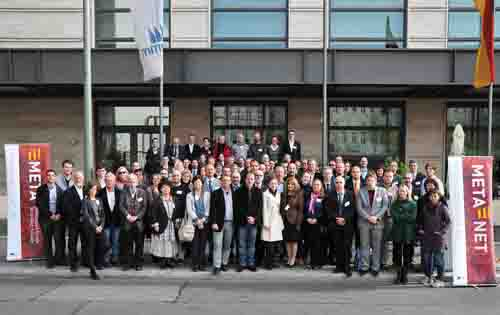
\includegraphics[width=\textwidth]{../_media/meta-net_team.jpg}
  \caption{Több mint 100 nyelvtechnológus szakértő -- a META-NET-ben részt vevő országok és nyelvek képviselői -- vitatta meg és véglegesítette a fehér könyvek sorozat főbb kérdéseit egy META-NET találkozón Berlinben, 2011. október 21-22-én. --- \textcolor{grey1}{About 100 language technology experts -- representatives of the countries and languages represented in META-NET -- discussed and finalised the key results and messages of the White Paper Series at a META-NET meeting in Berlin, Germany, on October 21/22, 2011.}}
\end{figure*}

\cleardoublepage

\bsection[A META-NET fehér könyvek sorozat -- The META-NET White Paper Series]{A META-NET fehér könyvek sorozat --- The META-NET\ \ \ \ \ \ White Paper Series}
\label{whitepaperseries}

\vspace*{-5mm}
\centering
  \setlength{\tabcolsep}{2em}
  \begin{tabularx}{\textwidth}{lllll} \toprule\addlinespace
  %\begin{tabulary}{170mm}{LLL} \toprule
    &angol & English & English& \\
&baszk & Basque & euskara& \\
  &bolgár & Bulgarian & български& \\
  &cseh & Czech & čeština& \\
  &dán & Danish & dansk& \\
  &észt & Estonian & eesti& \\
  &finn & Finnish & suomi& \\
  &francia & French & français& \\
  &galíciai & Galician & galego& \\
  &görög & Greek & ελληνικά& \\
   &holland & Dutch & Nederlands& \\
 &horvát & Croatian & hrvatski& \\
   &ír & Irish & Gaeilge& \\
 &izlandi & Icelandic & íslenska& \\
  &katalán & Catalan & català& \\
  &lengyel & Polish & polski& \\
  &lett & Latvian & latviešu valoda& \\
  &litván & Lithuanian & lietuvių kalba& \\
&magyar & Hungarian & magyar& \\
  &máltai & Maltese & Malti& \\
  &német & German & Deutsch& \\
  &norvég bokmål & Norwegian Bokmål & bokmål& \\
  &norvég nynorsk & Norwegian Nynorsk & nynorsk& \\
  &olasz & Italian & italiano& \\
  &portugál & Portuguese & português& \\
  &román & Romanian & română& \\
  &spanyol & Spanish & español& \\
  &svéd & Swedish & svenska& \\
  &szerb & Serbian & српски& \\
  &szlovák & Slovak & slovenčina& \\
  &szlovén & Slovene & slovenščina& \\
   \addlinespace \bottomrule
\end{tabularx}

\end{document}